\chapter{Cryogenic Instrumentation and Slow Control}
\label{ch:sp-cisc}

%\metainfo{Dual-phase section starts here [not a real fixme, just a landmark]}

\fixme{which portions of this are identical to what will be in the DP version of CISC? We need to note these portions. anne.  Please see added footnote - Glenn. I think I'll take it out of footnote and move it to main text. Tim hates footnotes! Anne}
%%%%%%%%
\section{Introduction} 


The \dfirst{cisc} consortium provides comprehensive monitoring for all detector  components and for \lar quality and behavior, and a control system for many of the detector components. %The structure of the \dword{cisc} consortium is quite complex.
The \dfirst{dpmod} uses the same control system and much of the same cryogenic instrumentation as the \dfirst{spmod}. A detailed list of instrumentation differences may be found in the corresponding chapter of Volume~4 of this \dword{tdr}. 

The consortium responsibilities are split into 
two main branches: cryogenics instrumentation and slow controls, as illustrated in  Figure~\ref{fig:cisc-subsystem-chart}. % provides a subsystem chart for the \dword{cisc} system. 

\begin{dunefigure}[CISC subsystem chart]{fig:cisc-subsystem-chart}
  {\dword{cisc} subsystem chart}
  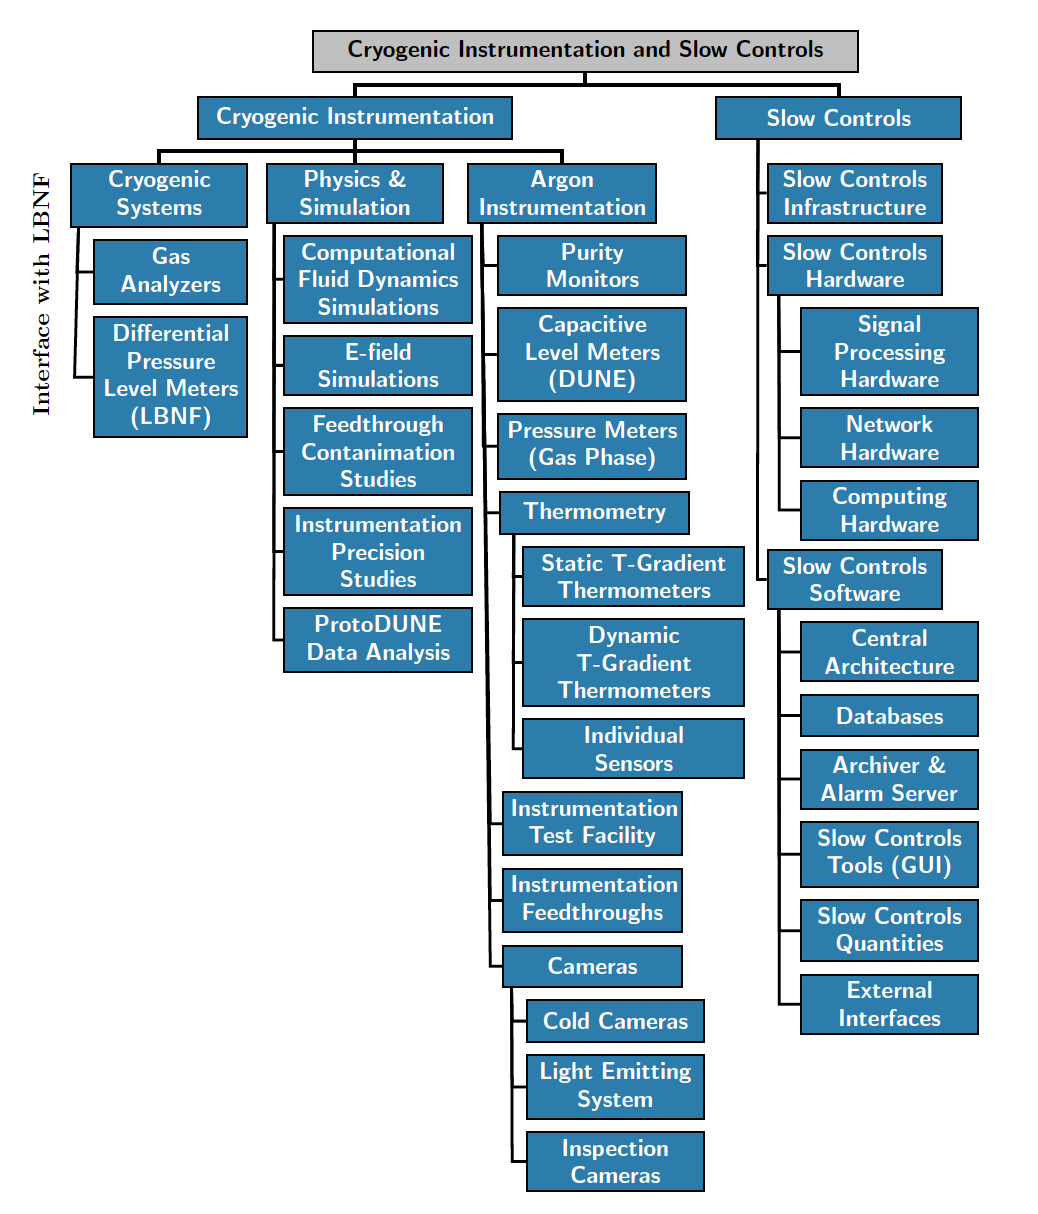
\includegraphics[width=0.8\textwidth]{graphics/CISC_scope_SP_2019Apr15.png}
\end{dunefigure}


%\dword{cisc} has  The former includes a set of instrumentation devices to monitor the quality and behavior of the \lar volume in the cryostat interior, ensuring correct functioning of the full cryogenics system and suitability of the \lar for good quality physics data. The second branch of \dword{cisc} is the slow controls (SC) system, in charge of monitoring and controlling most detector elements. %, as described below. 
%\fixme{Tim's text starts here}
Each element of \dword{cisc} contributes to the DUNE physics program primarily through the maintenance of high detector live time.  As described in Volume~2 of this \dword{tdr}, neutrino \dword{cpv} and resolution of the neutrino mass hierarchy over the full range of possible neutrino oscillation parameters will require at least a decade of running the \dword{fd}.  Similar requirements apply to searches for nucleon decay and \dword{snb} events from within our galaxy.  Throughout this long run-time the interior of any DUNE cryostat remains completely inaccessible.  No possibility exists for repairs to any components that could be damaged within the TPC structure; hence environmental conditions that present risks must be detected and reported quickly and reliably. 
 
Detector damage risks peak during the initial fill of a module with \lar, as temperature gradients take on their highest values during this phase.  Thermal contractions outside of the range of design expectations could result in broken \dword{apa} wires, \dwords{sipm} in \dwords{pd} that detach from the \dword{xarapu} light detectors, or poor connections at the cathode \dword{hv} feedthrough point that could lead to unstable \efield{}s.  These considerations lead to the need for %design of 
a robust temperature monitoring system for the detector, supplemented with liquid level monitors, and a high-performance camera system to enable visual inspection of the interior of the cryostat %through 
during the filling process.  These systems are fully described in Section~\ref{sec:fdsp-cryo-therm} of this chapter.
 
Argon purity must be established as early as possible in the filling process, a period in which gas analyzers are most useful, and must maintain an acceptable value, corresponding to a minimum electron drift lifetime of \SI{3}{ms}, throughout the data-taking period.  Dedicated  purity monitors (Section~\ref{sec:fdgen-slow-cryo-purity-mon}) 
provide precise lifetime measurements up to values of \SI{10}{ms}, the range over which electron attenuation most affects \dword{s/n} in the TPC.  The purity monitors and gas analyzers remain important even after high lifetime has been achieved as periodic detector ``top-off''  fills occur; the new \lar must be of very high quality as it is introduced into the cryostat.
 
The \dword{cisc} system must head off fault conditions that could develop in the \dword{detmodule} over long periods of running.  A drop in liquid level could place top sections of the \dword{fc} or bias \dword{hv} points  for the \dword{apa}s close enough to the gas-liquid boundary to trigger sparking events; the liquid level monitors must head off this possibility.  Very slow-developing outgassing phenomena could conceivably occur, with associated bubble generation creating another source of \dword{hv} breakdown events.  The cold camera system enables detection and identification of bubbling sites, and the development of mitigation strategies such as lower \dword{hv} operation for some period of time.  A more subtle possibility is the formation of quasi-stable eddies in argon fluid flow that could prevent positive argon ions from being cleared from TPC volume, resulting in space charge build up that would not otherwise be expected at the depth of the \dword{fd}.  The space charge could in turn produce distortions in the TPC drift field that degrade tracking and calorimetry performance.  The high-performance thermometry  of the DUNE \dword{cisc} system creates input for well developed complex fluid flow models described in Section~\ref{sec:fdgen-cryo-cfd} that should enable detection of  conditions associated with these eddies.
 
Finally, a high detector live-time fraction over multi-year operation cannot be achieved without an extensive system to monitor all aspects of detector performance, report this information in an intelligent fashion to detector operators, and archive the data for deeper offline studies.  Section~\ref{sec:sp-cisc-slowctrl} details the DUNE slow controls system designed for this task.
 
The baseline designs for all the \dword{cisc} systems have been used in \dfirst{pdsp}, % designs arethe baseline for all \lar instrumentation devices, and %requirements for 
and most design
parameters are extrapolated from these designs. The \dword{pdsp} data (and in some cases \dword{pddp} data) will therefore be used to validate the instrumentation designs and to understand their performance.

%\subsection{Components}
\subsection{Scope}
%\fixme{I am merging this with scope. Anne}

\subsubsection{Cryogenics Instrumentation}
%The devices included under c
Cryogenics instrumentation includes purity monitors,  various types of temperature monitors, and cameras with their associated light emitting systems. Also included are %components like 
gas analyzers and \lar level monitors that are directly related to the external cryogenics system, which have substantial interfaces with the \dword{lbnf}. \dword{lbnf} provides the needed expertise  for these systems and is responsible for the design, installation, and commissioning, while the \dword{cisc} consortium provides the resources and supplements labor as needed. 

A test facility for the instrumentation devices is also part of the cryogenics instrumentation.
 \dword{cisc} is responsible for design through commissioning in the \dword{spmod} %\dfirst{fd}.
of \lar instrumentation devices (purity monitors, thermometers, cameras, and light-emitting system, and their associated feedthroughs) and the \dword{citf}.

Cryogenics instrumentation %also 
requires significant engineering, physics and
simulation work, such as \efield simulations and cryogenics modeling
studies using \dfirst{cfd}. \efield simulations
%are required to 
identify desirable locations for instrumentation
devices in the cryostat, away from %so they are not in 
regions of high \efield, so that %and 
their presence does not induce large field distortions. 
% AC. What do we mean by distortions here ?
% Alternative: ``that their designs do not induce high \efields and risk of dielectric breakdown. ``
\dshort{cfd} simulations help identify %are needed to understand 
expected temperature, impurity, and velocity flow distributions and guide the placement and distribution of instrumentation devices inside the cryostat.

%%%%%%%%%%%%
\subsubsection{Slow Controls}
\label{sec:sp-cisc-slowctrl}
The slow controls portion of \dword{cisc} comprises three main components: 
%\fixme{figure shows 4, changed 3 to 4 here. [Carmen] we are changing the figure. [Glenn: figure changed]}
hardware, infrastructure, and software. The slow controls hardware and infrastructure comprises networking hardware, signal processing hardware, computing hardware, and associated rack infrastructure. The slow controls software provides, for every slow control quantity, the central slow controls processing architecture, databases, alarms, archiving, and control room displays.
% \fixme{this doesn't quite match the subsystem chart figure; Tim says close enough [Glenn: I made it a little closer]}

%\subsection{Scope} - moved up

%As described in the previous section, and shown schematically in Figure~\ref{fig:cisc-subsystem-chart}, the scope of the \dword{cisc} system spans a broad range of activities. 


%For slow controls, 
\dword{cisc} provides software and infrastructure for controlling and monitoring all detector elements that provide data on the health of the \dword{detmodule} or conditions important to the experiment, as well as  some related hardware. Slow controls includes the systems detailed below.

%\textbf{Slow controls base software and databases:}
Slow controls base software and databases are the central tools needed to develop
control and monitoring for various detector systems and interfaces. These include:
\begin{itemize}
\item base input/output software;
\item alarms, archiving, display panels, and similar operator interface tools; and 
\item slow controls system documentation and operations guidelines.
\end{itemize}

%\textbf{Slow controls for external systems:} 
Slow controls for external systems collect data from systems
external to the \dword{detmodule} and provide status monitoring for operators
and archiving. %These systems include 
They %will 
collect data on beam status, cryogenics status,
\dword{daq} status, facilities systems status, interlock
status bit monitoring (but not the actual interlock mechanism), ground
impedance monitoring, and possibly building and detector hall
monitoring, as needed.

%\textbf{Slow controls for detector hardware systems:}\
Slow controls for detector hardware systems %develop 
covers software interfaces for detector hardware devices, including:
\begin{itemize}
\item monitoring and control of all power supplies,
\item full rack monitoring (rack fans, thermometers and rack protection system),
\item instrumentation and calibration device monitoring (and control to the extent needed),
\item power distribution unit and computer hardware monitoring,
\item \dword{hv} system monitoring through cold cameras, and
\item detector components inspection %through 
using warm cameras.
\end{itemize}
%
%\textbf{Slow controls hardware:} 
\dword{cisc} will develop, install, and commission any hardware related to rack monitoring and control. Most power supplies may only need a cable from the device
to an Ethernet switch, but some power supplies might need special cables (e.g., GPIB or RS232) for communication. The \dword{cisc} consortium is responsible for providing these control cables.

%In addition to the listed activities, 
\dword{cisc} %also has 
has additional activities outside the scope of the consortium that require coordination with other groups. This is discussed in Section~\ref{sec:interfaces}.

%\subsection{Requirements}
\subsection{Design Considerations}

%Some common 
Important design considerations for instrumentation devices include stability, reliability, and longevity, so that the devices can survive for a period of at least \dunelifetime. %For any device to have 
Such longevity %a long lifetime 
is uncommon for any device, so the overall design allows replacement of devices where possible. %A requirement common to every element inside the cryostat is that 
DUNE requires the \efield  on any instrumentation devices inside the cryostat to be less than \localefield to minimize the risk of dielectric breakdown in \lar. %To avoid confusing event reconstruction, we include another important design parameter that should be evaluated in \dword{pdsp}: the maximum noise level induced by instrumentation devices on the readout electronics that can be tolerated.
A consideration important for event reconstruction is the maximum noise level induced by instrumentation devices that the readout electronics  can tolerate. \dword{pdsp} is evaluating this.  Tables~\ref{tab:fdgen-slow-cryo-requirements-1} and \ref{tab:fdgen-slow-cryo-requirements-2} show the full set of specifications %requirements for the \dword{cisc} subsystems.
that relate to the \dword{cisc} subsystems.

Data from purity monitors and different types of thermometers will be used to validate the \lar fluid flow model. 
%A number of requirements drive the design parameters on the precision and granularity in their distribution across the cryostat. 
A number of requirements drive the design parameters for the precision and granularity of monitor distribution across the cryostat. 
For example, the electron lifetime measurement precision must be \SI{1.4}{\%} to keep the bias on the charge readout in the \dword{tpc} below \SI{0.5}{\%} at \SI{3}{ms} lifetime. For thermometers, the %requirements 
parameters are driven by the \dshort{cfd} simulations based on \dword{pdsp} design.
The temperature measurement resolution must be less than \SI{2}{mK}, and the relative precision of those measurements must be less than \SI{5}{mK}. The resolution is defined as the temperature RMS for individual measurements and is driven by the electronics. The relative precision also includes the effect of reproducibility for successive immersions in \dword{lar}. 
The relative precision is particularly important in order to characterize %because 
gradients below \SI{20}{mK}. % should be characterized.  
As will be described below, the laboratory calibration data and the recent analysis of thermometer instrumentation data from \dword{pdsp} shows that a \SI{2.5}{mK} relative precision is achievable. 

The level meters must have a precision of 0.1\% over \SI{14}{m} (i.e., \SI{14}{mm}) for measurement accuracy during filling. This precision is also sufficient to ensure that the \dword{lar} level stays above the \dwords{gp} of a \dfirst{sp} module. As shown in Table~\ref{tab:fdgen-slow-cryo-requirements-2}, several requirements drive the design of cold and warm cameras and the associated light emitting system. The components of the camera systems must not contaminate the \lar or produce bubbles % when the \dword{hv}
so as  to avoid  increasing the risk of \dword{hv} discharge. Both cold and warm cameras must provide coverage of at least \SI{80}{\%} of the \dword{tpc} volume 
\fixme{An illustration showing where all these instruments go would be helpful. Anne. Locations are not defined yet for some of the devices [Carmen and Glenn] -- can't fix by deadline.}
with a resolution of \SI{1}{cm} for cold cameras and \SI{2}{mm} for warm cameras on the \dword{tpc}.
% CEL: my 'fix me' with details, removed. Wanted to hold 
% if needed later in the document. 

For the cryogenic test facility, a cryostat with a capacity of only \num{0.5} to approximately \SI{3}{m^3} %cubic meter is reasonable because 
will suffice and will keep turn-around times and filling costs %are 
lower. % for smaller cryostats. 
For gas analyzers, the operating range must allow establishment of useful electron lifetimes;
% is an important requirement; 
details  are in Table~\ref{tab:fdgen-slow-cryo-requirements-1}.

For slow controls, the system must %be designed to 
be sufficiently robust to monitor 
a minimum of 150,000  variables per \dword{detmodule}, and 
support a broad range of monitoring and archiving rates. The system must also %be capable of an 
interface with a large number of detector subsystems and %to 
establish two-way communication with them for control and monitoring. 

% \fixme{Anne added input of generated SP-CISC specifications table here. Need to compare contents and make sure the generated one contains all the right information for the CISC-specific items. The top-level ones that apply are now there: top 5 plus the CISC-selected ones) {\bf Anselmo and Glenn are still working on checking contents (2019-01-11)} -- DONE}
% This file is generated, any edits may be lost.

\begin{longtable}{p{0.14\textwidth}p{0.13\textwidth}p{0.18\textwidth}p{0.22\textwidth}p{0.20\textwidth}}
\caption{Specifications for SP-CISC \fixmehl{ref \texttt{tab:spec:SP-CISC}}} \\
  \rowcolor{dunesky}
       Label & Description  & Specification \newline (Goal) & Rationale & Validation \\  \colhline

   \newtag{SP-FD-1}{ spec:min-drift-field }  & Minimum drift field  &  $>$\,\SI{250}{ V/cm} \newline ( $>\,\SI{500}{ V/cm}$ ) &  Lessens impacts of $e^-$-Ar recombination, $e^-$ lifetime, $e^-$ diffusion and space charge. &  ProtoDUNE \\ \colhline
    
   
  \newtag{SP-FD-2}{ spec:system-noise }  & System noise  &  $<\,\SI{1000}\,e^-$ &  Provides $>$5:1 S/N on induction planes for  pattern recognition and two-track separation. &  ProtoDUNE and simulation \\ \colhline
    
   
  \newtag{SP-FD-3}{ spec:light-yield }  & Light yield  &  $>\,\SI{20}{PE/MeV}$ (avg), $>\,\SI{0.5}{PE/MeV}$ (min) &  Gives PDS energy resolution comparable that of the TPC for 5-7 MeV SN $\nu$s, and allows tagging of $>\,\SI{99}{\%}$ of nucleon decay backgrounds with light at all points in detector. &  Supernova and nucleon decay events in the FD with full simulation and reconstruction. \\ \colhline
    
    \\ \rowcolor{dunesky} \newtag{SP-FD-4}{ spec:time-resolution-pds } & Name: Time resolution \\
    Description & The time resolution of the photon detection system shall be less than 1 microsecond in order to assign a unique event time.   \\  \colhline
    Specification (Goal) &  $<\,\SI{1}{\micro\second}$  ( $<\,\SI{100}{\nano\second}$ ) \\   \colhline
    Rationale &   Enables \SI{1}{mm} position resolution for \SI{10}{MeV} SNB candidate events for instantaneous rate $<\,\SI{1}{m^{-3}ms^{-1}}$.  \\ \colhline
    Validation &   \\
   \colhline

   \newtag{SP-FD-5}{ spec:lar-purity }  & Liquid argon purity  &  $<$\,\SI{100}{ppt} \newline ($<\,\SI{30}{ppt}$) &  Provides $>$5:1 S/N on induction planes for  pattern recognition and two-track separation. &  Purity monitors and cosmic ray tracks \\ \colhline
    
    \\ \rowcolor{dunesky} \newtag{SP-FD-15}{ spec:lar-n-contamination } & Name: LAr nitrogen contamination \\
    Description & The nitrogen contamination in the LAr shall remain below 25 ppm in order not to significantly affect the number of photons that reach the detectors (for both fast and late light components).   \\  \colhline
    Specification &  $<\,\SI{25}{ppm}$ \\   \colhline
    Rationale &   Maintain \SI{0.5}{PE/MeV} PDS sensitivity required for triggering proton decay near cathode.  \\ \colhline
    Validation & In situ measurment  \\
   \colhline

    
   
  \newtag{SP-FD-18}{ spec:cryo-monitor-devices }  & Cryogenic monitoring devices  &   &  Constrain uncertainties on detection efficiency, fiducial volume. &  ProtoDUNE \\ \colhline
    
   
  \newtag{SP-FD-25}{ spec:non-fe-noise }  & Non-FE noise contributions  &  $<<\,\SI{1000}{enc} $ &  High S/N for high reconstruction efficiency. &  Engineering calculation and ProtoDUNE \\ \colhline
    

   
  \newtag{SP-CISC-1}{ spec:inst-noise }  & Noise from Instrumentation devices  &  $\ll\,\SI{1000}\,e^- $ &  Max noise for 5:1 S/N for a MIP passing near cathode; per SBND and DUNE CE &  ProtoDUNE \\ \colhline
    
    \\ \rowcolor{dunesky} \newtag{SP-CISC-2}{ spec:inst-efield } & Name: Max. E field near instrumentation devices \\
    Description & The maximum field near instrumentation devices should be $<\,\SI{30}{kV/cm}$ to avoid dielectric breakdowns.   \\  \colhline
    Specification (Goal) &  $<\,\SI{30}{kV/cm}$  ( $<\,\SI{15}{kV/cm}$ ) \\   \colhline
    Rationale &   Significantly lower than max field of 30 kV/cm per DUNE HV   \\ \colhline
    Validation & 3D electrostatic simulation  \\
   \colhline

   \newtag{SP-CISC-3}{ spec:elec-lifetime-prec }  & Precision in electron lifetime  &  $<\,$1.4\% \newline ($<\,$1\%) &  Required for accurate charge reconstruction per DUNE-FD Task Force report. &  ProtoDUNE-SP and ITF \\ \colhline
    
   
  \newtag{SP-CISC-4}{ spec:elec-lifetime-range }  & Range in electron lifetime  &  \SIrange{0.04}{10}{ms} in cryostat, \SIrange{0.04}{30}{ms} inline &  Slightly beyond best values observed so far in other detectors.  &  ProtoDUNE-SP and CITF \\ \colhline
    
   \newtag{SP-CISC-11}{ spec:temp-repro }  & Precision: temperature reproducibility  &  $<\,\SI{5}{mK}$ \newline (\SI{2}{mK}) &  Enables validation of CFD models, which predicts gradients below 15 mK &  ProtoDUNE-SP and ITF \\ \colhline
    
   \newtag{SP-CISC-14}{ spec:temp-stability }  & Temperature stability  &  $<\,\SI{2}{mK}$ at all places and times \newline ( Match precision requirement at all places, at all times ) &  Measure the temp map with sufficient precision during the entire duration &  ProtoDUNE-SP \\ \colhline
    
    \\ \rowcolor{dunesky} \newtag{SP-CISC-27}{ spec:camera-cold-coverage } & Name: Coverage \\
    Description & The cold cameras are required to cover at least 80\% of the exterior of HV surfaces.   \\  \colhline
    Specification (Goal) &  $>\,$80\% of HV surfaces  ( \num{100}\% ) \\   \colhline
    Rationale &     \\ \colhline
    Validation &   \\
   \colhline

   \newtag{SP-CISC-51}{ spec:slowcontrol-alarm-rate }  & Slow control alarm rate  &  $<\,$150/day \newline ( $<\,$50/day ) &  Alarm rate low enough to allow response to every alarm. &  Detector module; depends on experimental conditions \\ \colhline
    
   \newtag{SP-CISC-52}{ spec:slowcontrol-num-vars }  & Total No. of variables  &  $>\,\num{150000}$ \newline (\SIrange{150000}{200000}{}) &  Scaled from ProtoDUNE-SP &  ProtoDUNE-SP and CITF \\ \colhline
    
    
   \newtag{SP-CISC-54}{ spec:slowcontrol-archive-rate }  & Archiving rate  &  \SI{0.02}{Hz} \newline ( Broad range \SI{1}{Hz} to \num{1} per few min. ) &  Archiving rate different for each variable, optimized to store important information  &  ProtoDUNE-SP \\ \colhline
    


\label{tab:specs:SP-CISC}
\end{longtable}


\begin{dunetable}
[Specifications for CISC subsystems]
{p{0.45\linewidth}p{0.25\linewidth}p{0.25\linewidth}}
{tab:fdgen-slow-cryo-requirements-1}
{List of specifications for the different CISC subsystems}   
Quantity/Parameter				                             & Specification			                                        & Goal		                                              \\ \toprowrule                     
Noise from Instrumentation devices				             & $\ll$ \elecnoisefe                                      & 
\\ \colhline                     
Max. \efield near instrumentation devices				     & <\localefield			                                                & <15 kV/cm		                                          \\ \colhline                     
\textbf{Purity Monitors}	                                             &                                                                      &                                                         \\ \colhline                      
Precision in electron lifetime				                 & <1.4\% at 3~ms,  <4\% at 9~ms,  relative differences <2.5\%			                                            & < 1\%		                                              \\ \colhline                     
Range in electron lifetime				                     & 0 - 10 ms  			                    & (0 - 30 ms inline)       
\\ \colhline                         
Longevity				                                     & \dunelifetime			                                                    & > \dunelifetime		                                      \\ \colhline                     
Stability				                                     & Match precision requirement at all places/times			    & %Match precision requirement at all places/times  
\\ \colhline  	                   
Reliability				                                     & Daily Measurements			                                        & Measurements %capable of being 
as needed	  \\ \colhline                         
\textbf{Thermometers}	                                             &                                                                      &                                                         \\ \colhline                      
Vertical density of sensors for T-gradient monitors			 & > 2 sensor/m			                                                & > 4 sensors/m		                                      \\ \colhline                 
2D horizontal density for top/bottom individual sensors		 &  1 sensor/5(10) m 			                                        &  1 sensor/3(5) m 		                                  \\ \colhline                     
Resolution of temperature measurements				         & < 2 mK			                                                    & <0.5 mK		                                          \\ \colhline                         
Precision: temperature reproducibility 				         & < 5 mK			                                                    & 2 mK		                                              \\ \colhline                     
Reliability				                                     & 80\% (in 18 months)			                                        & 50\% (during 20 years)		                              \\ \colhline                     
Longevity				                                     & > 18 months			                                                & > 20 years		                                      \\ \colhline                         
Stability 	  &  < \SI{2}{mK} at all places and times	 &   Match precision requirement at all places/times \\ \colhline                 
Discrepancy between lab and  in situ calibrations for temperature sensors			             & < 5 mK			                                                    & < 3 mK		                                          \\ \colhline                           
Discrepancy between measured temperature map and CFD simulations in \dword{pdsp}	 & < 5 mK & %< 5 mK		     
\\ \colhline                             
\textbf{Gas Analyzers}	   &   &  \\ \colhline            
Operating Range O2	 & 0.2 (air) to 0.1 ppt  & %Air (0.2) to 0.1 ppt
\\ \colhline    
Operating Range H2O				                             & %Nominally Air to sub ppb levels, depending on species of contaminant	
Nom. air to sub ppb; contaminant-dependent & %Air to sub ppb.  levels, depending on species of contaminant	          
\\ \colhline           
Operating Range N2				                             & Nominally Air Nom. air to sub ppb; contaminant-dependent	& %Air to sub ppm.
\\ \colhline             
Precision: 1 sigma at zero				                     & %depends on the range of the gas analyzer
per gas analyzer range
& %depends on the range of the gas analyzer		                     
\\ \colhline     
Detection limit: 3 sigma & Different analyzer modules needed to cover entire range	& %Different Gas analyzer modules are needed to cover the entire range 
\\ \colhline           
Stability   & <\% of full scale range.		 & %<\% of full scale range.
\\ \colhline         
Longevity		 & >10 years	  & %10 years  
\\   \colhline
\textbf{Pressure Meters (GAr)}	          &    &          \\ \colhline            
Relative precision (DUNE side)		   & 0.1~mbar	& %0.1\% over 14 m (14 mm)
\\ \colhline  
Absolute precision (DUNE side)		   & <5~mbar	& %0.1\% over 14 m (14 mm)
\\  
\end{dunetable}


\begin{dunetable}
[Specifications for CISC subsystems]
{p{0.45\linewidth}p{0.25\linewidth}p{0.25\linewidth}}
{tab:fdgen-slow-cryo-requirements-2}
{List of specifications for the different CISC subsystems}   
Quantity/Parameter		     & Specification	  & Goal   \\ \toprowrule   
\textbf{Level Meters}	          &    &          \\ \colhline            
Precision (LBNF scope)		   & 0.1\% over 14 m (14 mm)			                                    & %0.1\% over 14 m (14 mm)
\\ \colhline           
Precision (capacitive level meters, \dword{dune} scope) & 1~cm  &  <5 mm
\\ \colhline         
Longevity (all)		  & 20 years	   & > 20 years		                                                  \\ \colhline     
\textbf{Cold cameras}	                                             &                                                                      &                                                                     \\ \colhline        
Coverage				                                     & 80\% of the exterior of HV surfaces			                        & 100\% 	                                                          \\ \colhline         
Frames per second	   & yet to be defined	  & %yet to be defined
\\ \colhline             
Resolution 	 & 1 cm on the TPC	 & yet to be defined
\\ \colhline           
Duty cycle	  & yet to be defined	 & %yet to be defined
\\ \colhline         
longevity			 & > 18 months			                                                & > 20 years		                                                  \\ 
\textbf{Inspection cameras}	     &                                                                      &                                                                     \\ \colhline        
Coverage	 & 80\% of the TPC		  & yet to be defined		                                              \\ \colhline         
Frames per second		   & yet to be defined	   & %yet to be defined	
\\ \colhline             
Resolution 	  & 2 mm on the TPC			                                            & yet to be defined		                                              \\ \colhline           
heat transfer	  & no generation of bubbles			                                & 	%no generation of bubbles	
\\ \colhline         
longevity			  & > 18 months			                                                & > 20 years		                                                  \\ \colhline         
\textbf{Light emitting system}	                                     &                                                                      &                                                                     \\ \colhline        
radiant flux     & > 10 mW/sr		 & 100 mW/sr \\ \colhline         
power				     & < 125 mW/LED			                                        & %\dword{alara}	
\\ \colhline           
wavelength	   & red/green		 & IR/white	   \\ \colhline         
longevity	  & > 18 months (for cold cameras) 			                            & > 20 years		                                              \\ \colhline         
\textbf{Cryogenics Instrumentation Tests Facility}	                 &                                                                      &                                                                     \\ \colhline            
Dimensions		  & 0.5 to 3  cubic meters 			                                    & %0.5-3 cubic meters
\\ \colhline             
Temperature stability	 & $\pm$1K	 & %+- 1K
\\ \colhline                                       
Turn-Around time	 & $\sim\,$9 days   & 9 days 	  \\ \colhline                                       
LAr purity		   & O2, H2O: low enough  to measure drifting electrons of devices under test, $\sim\,\SI{0.5}{ms}$.    N2: ppm for scintillation light tests. 	        &  >1.0 ms                                                            \\ \colhline
\textbf{Slow Controls}		                                         &                                                                      &                                                                     \\ \colhline
Alarm rate	  & <150/day			                                                    &  < 50/day                                                           \\ \colhline
Total No. of variables per \dword{detmodule}				                         & 150,000			                                                    &  150,000 - 200,000                                                   \\ \colhline
Server rack space				                             & 2 racks			                                                    &  3 racks                                                            \\ \colhline
Archiving rate 				                                 & 0.02 Hz			                                                    &  Broad range 1 Hz  to 1 per few min.                                \\ \colhline
Near Detector Status & Beam conditions and detector status	                                &  Full beam and detector status                                      \\          
\end{dunetable}                                  

%%%%%%%%
\subsection{Fluid Dynamics Simulation}
\label{sec:fdgen-cryo-cfd}

Proper placement of purity monitors, thermometers, and liquid level monitors within the \dword{detmodule} requires knowing how \lar flows within the cryostat, given its fluid dynamics, heat and mass transfer, and distribution of impurity concentrations. Fluid motion within the cryostat is driven primarily by small changes in density caused by thermal gradients within the fluid, although pump flow rates and inlet and outlet locations also contribute. Heat sources include exterior heat from the surroundings, interior heat from electronics, and heat flow through the pump inlet. In principle, purity monitors can be placed throughout the cryostat to determine if the argon is pure enough for experimentation. However, fluid flow, \dword{hv}, cost, and space constraints limit the distribution of these monitors in the cryostat.

%However, some areas inside the cryostat are off limits for such monitors. 
% \fixme{anne moved prev pgraph up --- looks good [Glenn, Carmen, Sowjanya]}

To determine the purity of the argon in regions where experimental data is unavailable, \dword{cfd} simulations can be used to better understand and quantify impurity levels. The overall goal of the \dword{cfd} simulations
%\dword{dune} \dword{fd} 
%for the \dword{spmod} 
is to better understand and predict the fluid (in either a liquid and vapor state) motions and the implications for the detector performance. % of the detectors. 
The fluid flow behavior can be determined by simulating \dword{lar} flow within a \dword{detmodule} %the detector 
using Siemens Star-CCM$+$\footnote{https://mdx.plm.automation.siemens.com/star-ccm-plus}, a commercially available \dword{cfd} code.  Such a model must properly define the fluid characteristics, solid bodies and fluid-solid interfaces, and provide a means for measuring contamination, while still maintaining reasonable computation times. In addition, these fluid dynamics simulations are compared with available experimental data (see Section~\ref{sec:cfdvalid}) to assess simulation accuracy and credibility. 

%\fixme{seems like the above is sp/dp independent but the next stuff isn't. anne. The text has been modified [Carmen and Glenn] --- we think this is fixed.}
Although simulation of the \dword{detmodule} presents challenges, %there are 
acceptable simplifications can %to 
accurately represent the fluid, the interfacing solid bodies, and variations of contaminant concentrations. Because of the magnitude of thermal variation within the cryostat, modeling of the \lar is simplified by using constant thermophysical properties, calculating buoyant force with the Boussinesq Model (using a constant density for the fluid with application of a temperature-dependent buoyant force), and a standard shear stress transport turbulence model. Solid bodies that touch the \lar include the cryostat wall, cathode planes, anode planes, \dword{gp}, and \dword{fc}. As in previous \dword{cfd} models of the \dword{dune} 35-ton prototype and \dword{pdsp}%{protodune} 
%\fixme{Another abbreviation that may need to be coded in Latex. {\em Or it might be better to remove repeated references to SDSU and FNAL here. Why are we focusing attention in the technical section on distinguishing between FNAL and SDSU CFD simulations? --Glenn. Anselmo: I think we can remove SDSU in the previous sentence and also below( and FNAL). Institutions should be only mentioned in the section about organization and management. This was probably important when SDSU was not part of the consortium. } {\bf Carmen working on this.}}
\cite{bib:docdb5915}, the \dword{fc} planes, anode planes, and \dword{gp} can be represented by porous bodies. Because impurity concentration and electron lifetime do not affect fluid flow, these variables can be simulated as passive scalars, as is commonly done for smoke released \cite{cfd-1} 
in air or dyes released in liquids.

% top pgraph in section was taken from here. Anne

Discrepancies between real data and simulations may affect detector performance. % because 
Simulation results contribute to decisions about where to place sensors and monitors, and to %as well as 
the definitions of various calibration quantities. Methods of mitigating such risks include well established convergence criteria, sensitivity studies, and comparison to results of previous \dword{cfd} simulation work. Moreover, the simulation will be improved with input from temperature measurements and validation tests from \dword{pdsp}. %{protodune} 

% \fixme{Must find better pictures. Just use this for now (not sure who wrote this) anne asks - why describe right side then left? [Carmen] already fixed (by Anne)}
\begin{dunefigure}[\dshort{cfd} example]{fig:cfd-example}
  {Distribution of temperature on a plane intersecting an inlet (left) and halfway between an inlet and an outlet (right), as predicted by previous \dshort{cfd} simulations (from~\cite{bib:docdb5915}). (See Fig.~\ref{fig:cfd-example-geometry} for geometry.)}
  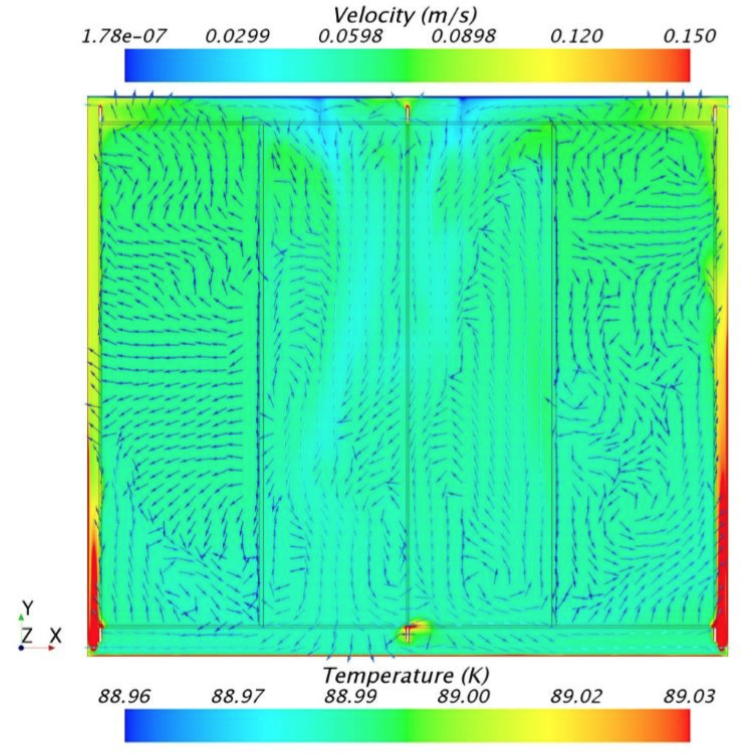
\includegraphics[height=0.4\textwidth]{cisc_cfd_inlet_z52.png}
  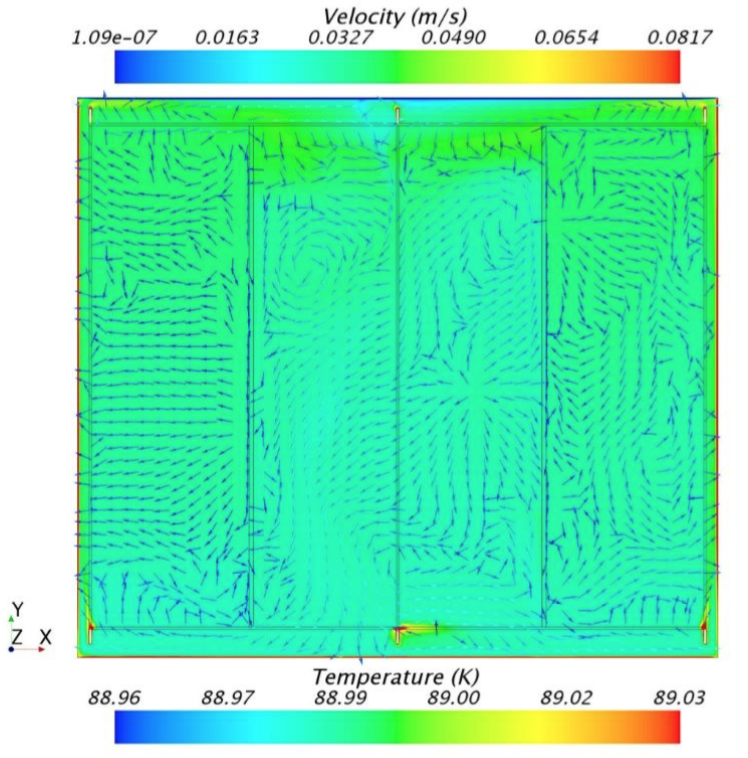
\includegraphics[height=0.4\textwidth]{cisc_cfd_outlet_z0.png}
\end{dunefigure}

Figure~\ref{fig:cfd-example} shows an example of the temperature
distribution on a plane intersecting a \lar inlet and at a
plane halfway between an inlet and an outlet; 
the geometry used for
this simulation is shown in Figure~\ref{fig:cfd-example-geometry}\footnote{the inlet and outlet map has recently changed; it now consists of two rows of 64 inlets each at each longer side of the cryostat and four outlets along the shorter sides (drift direction) of the cryostat.}. Note the plume of higher temperature \lar between the walls and
the outer \dword{apa} on the inlet plane. The current placement of instrumentation in
the cryostat as shown in Figure~\ref{fig:cisc-tsensor-map} was determined using temperature and impurity distributions from previous simulations.
%\fixme{might make sense to move CFD down closer to fig 1-11? anne. We cannot figure out how to do this. [Glenn]. SG: we prefer to keep it here. }

\begin{dunefigure}[\single \dword{cisc} geometry layout]{fig:cfd-example-geometry}
  {Layout of the \single \dword{tpc} within the cryostat (top) and positions of \dword{lar} inlets and outlets (bottom) as modeled in the \dword{cfd} simulations~\cite{bib:docdb5915}. The $y$ axis is vertical and the $x$ axis is parallel to the \dword{tpc} drift direction. Inlets are shown in green and outlets are shown in red.}
  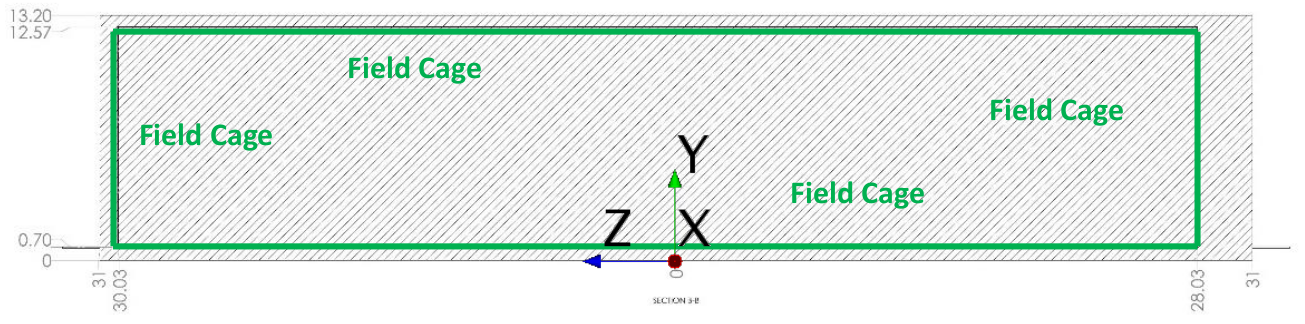
\includegraphics[width=0.7\textwidth]{cisc_cfd_cryostat-layout.png}
  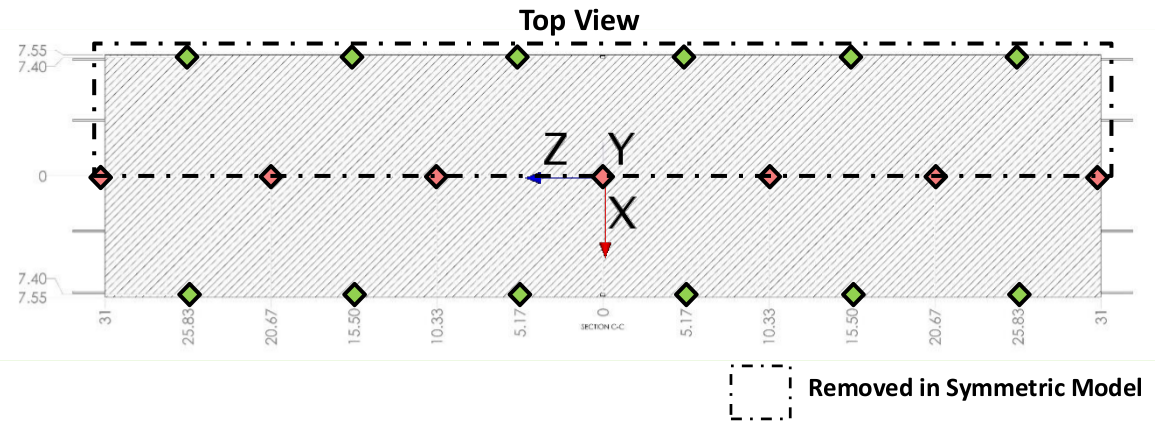
\includegraphics[width=0.7\textwidth]{cisc_cfd_inlet-outlet-layout.png}
\end{dunefigure}

The strategy for  future \dword{cfd} simulations begins with understanding the performance of the \dword{pdsp} cryogenics system and modeling the \dwords{detmodule} to derive specifications %requirements 
for instrumentation. We are pursuing a prioritized set of studies to help determine the requirements for other systems. We plan to 
\begin{itemize}
\item review the \dword{dune} \dword{fd} cryogenics system design and verify the current implementation in simulation %to ensure that the model represents what will be built.
to ensure that the simulation represents the actual design.
\item 
model the \dword{pdsp} liquid and gas regions with the same precision as the \dword{fd}. Presently, we have only the liquid model, which is needed to interpret the thermometer data. The gas model is needed to see how to place thermometers in the ullage and verify the design of the gaseous argon purge system.
% \item Perform a \dword{cfd} study to determine the feasibility of a wier for DP; this helps to determine if it can be used to clean the \dword{lar} surface before the extraction grid is submerged in the DP module.
\item verify the \dword{cfd} model for the \dword{spmod} in a simulation performed by LBNF; this defines the requirements for instrumentation devices (e.g., thermometry).
% \item Model the \dword{pddp} liquid and gas regions with the same precision as the \dword{fd}.
\end{itemize}

\begin{dunetable}
[\dword{cfd} parameters for \dword{protodune}]
{p{0.25\textwidth}p{0.15\textwidth}p{0.5\textwidth}}
{tab:fdgen-cisc-CFDparam}
{\dword{cfd} input parameters for \dword{protodune}}   


Parameter  &	Value &	Comments \\ \toprowrule
Cryostat height
&
7.878 m
&
Measured with laser (1 cm error approx.)
\\ \toprowrule	
LAr surface height
&
7.406 m
&
Measured by capacitive level meter ($<1$ cm error)
\\ \toprowrule	
Ullage pressure		
&
1.045 bar
&
Measured by pressure gauges
\\ \toprowrule
\lar surface temperature
&
87.596 K
&
Computed using ullage pressure and \cite{larpropertiesbnl}%(Luke to add to bib) \linebreak
%https://lar.bnl.gov/properties/basic.html\#phase
\\ \toprowrule
\lar inlet temperature
&
outlet + 0.2 K
&
Estimated
\\ \toprowrule
\lar flow rate per pipe
&
0.4170025 kg/s
&
\\ \toprowrule		
Heat flux 
&
\SI{5.76}{W/m^2}
&
This is the heat flux from all four walls as well as the ground
\\ \toprowrule
Vapor being drawn from the chimneys
&
5-7 gr/sec
&
Among all chimneys
\\
\end{dunetable}
%%%%%%%%%%%%%%%%%%%%
\subsubsection{Validation in \dword{protodune}}
\label{sec:cfdvalid}
\dword{pdsp} has collected data to validate the \dword{cfd} using: % already installed instrumentation.
\begin{itemize}
\item static and dynamic T-gradient thermometers, 
\item individual temperature sensors placed in the return \lar inlets, 
\item two \twod grids of individual temperature sensors installed below the bottom ground planes and above the top ground planes, 
\item a string of three purity monitors vertically spaced from near the bottom of the cryostat to just below the \lar surface
\item two pressure sensors (relative and absolute) in the argon gas
\item H$_{2}$O, N$_{2}$, and O$_{2}$ gas analyzers, 
\item \dword{lar} level monitors, and
\item standard cryogenic sensors including pressure transducers, individual temperature sensors placed around
the cryostat on the membrane walls, and recirculation flow rates transducers.
\end{itemize}

% \fixme{I notice the list format here is [was?] somewhat different from other chapters. We may need to go through and make punctuation at the end of each item and at the end of the list consistent throughout the manuscript. {\em (I have gone through and attempted to make all lists consistent with section 4.5 (``Lists'') of the \dword{dune} TDR Guide, but this still needs to be revisited. --Glenn)}}

%These devices are running and have already produced 
The data, which has been logged through the \dword{pdsp} slow control system \cite{pdspdcs_proc}, is available for offline analysis. %\fixme{reference? -- reference added} 

\begin{dunefigure}[Streamlines for \lar flow inside  \dword{pdsp}]{fig:cisc-cfd-larflow-inlets}
  {Streamlines for \lar flow inside  \dword{pdsp}}
  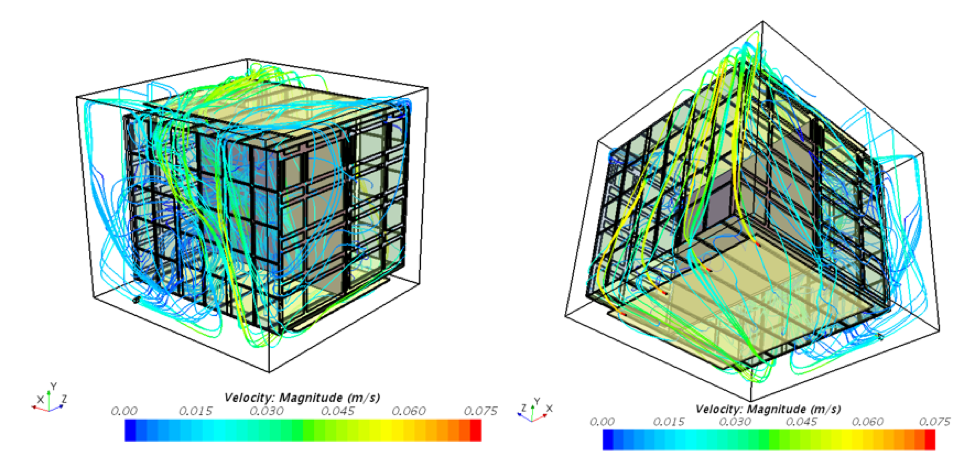
\includegraphics[width=0.8\textwidth]{cisc_cfd_larflow-inlets.png}
\end{dunefigure}

In parallel, \dword{cisc} has produced a \dword{pdsp} \dword{cfd} model %has been produced 
with input from \dword{pdsp} measurements (see Table  \ref{tab:fdgen-cisc-CFDparam}). Streamlines\footnote{In fluid mechanics, a streamline is a line that is everywhere tangent to the local velocity vector. For steady flows, a streamline also represents the path that a single particle of the fluid will take from inlet to exit.} from the current  simulation (Figure~\ref{fig:cisc-cfd-larflow-inlets}) show the flow paths from the four cryostat inlets to the outlet. The validation of this model consists of an iterative process in which several versions of the \dword{cfd} simulation, using different input parameters, eventually %will %be produced to 
converge %on 
to a reasonable agreement with data from instrumentation devices. Preliminary results for the comparison of vertical temperature profiles already exist. Figure~\ref{fig:cisc-cfd-valid} shows the fluid temperature measured by the dynamic T-gradient thermometer and compares it against the current \dword{pdsp} \dword{cfd} model, with parameters shown in Table~\ref{tab:fdgen-cisc-CFDparam}.
%\fixme{We still need to confirm this table is indeed showing input parameters to the iteration procedure for comparison with temperature probes. Anselmo: I'll ask SDSU today. {\bf Anselmo working on this.}}. 
The agreement is already quite good. %, which indicates that the current  \dword{pdsp} \dword{cfd} model is reasonable. 

%The comparison with the dynamic T-gradient monitor data is just the first step in the validation. As described below, data from purity monitors and other temperature probes will be also used. Furthermore, cryostat conditions will be changed deliberately such that several points of comparison exist, allowing for further refinement of the \dword{pdsp} \dword{cfd} model.  

\begin{dunefigure}[Comparison of \dword{pdsp} temperature data and CFD simulations]{fig:cisc-cfd-valid}
  {Comparison of \dword{pdsp} temperature data and \dword{cfd} simulations.}
  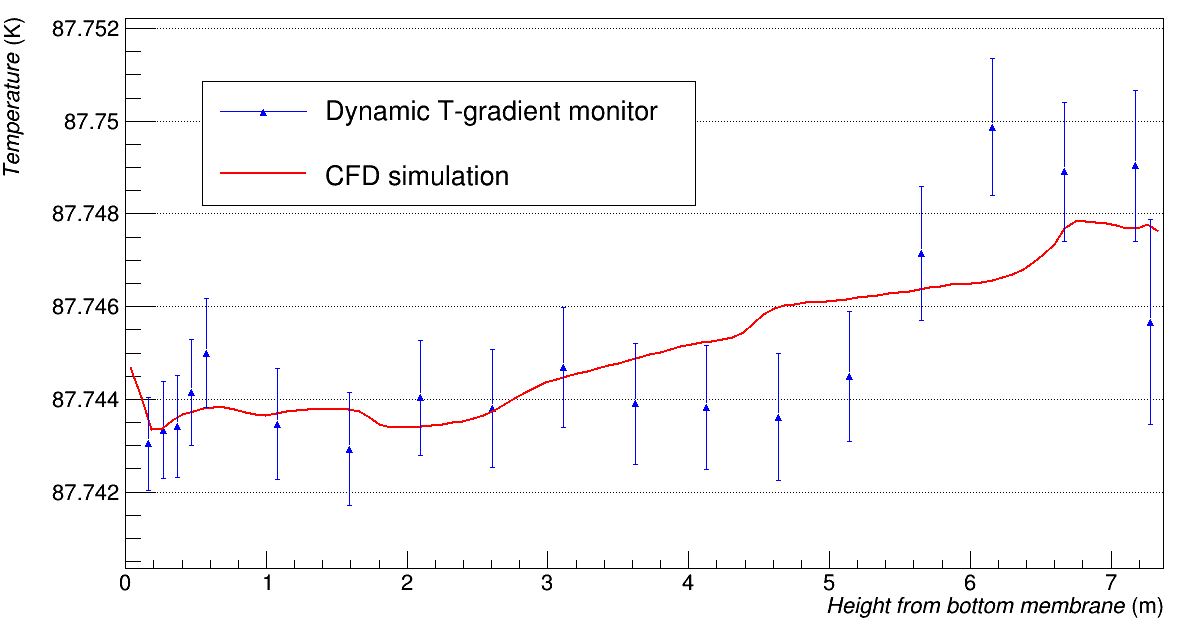
\includegraphics[width=0.6\textwidth]{cisc_CFD_valid_v1.png}
\end{dunefigure}


%Additional dedicated tests are also planned to validate the \dword{cfd} under various deliberate changes of the cryostat environment; measuring the instrumentation response may help establish the validity of the \dword{cfd} model. The \dword{cfd} predicts a reasonable response for more than one set of initial conditions, which is reassuring.   These tests were not attempted during the beam run because even controlled changes of the cryostat environment could have undesirable effects. Some possible additional tests include pump/recirculation manipulations such as pump on/off, pumping speed change, and bypassing filtration. Additionally, changes in the pressure can be induced by setting the cryostat pressure set point to a higher (or lower) value\footnote{The HV could be ramped down for this exercise because dropping the pressure too fast might provoke boiling of the \lar near the surface.} for a specified time while monitoring the instrumentation. Any change in pressure could change the temperatures everywhere in the cryostat. Studying the rate of this change, as detected in the various vertical heights of the cryostat, might provide interesting constraints on the \dword{cfd} model.
The \dword{cfd} reassuringly predicts a
reasonable response for more than one set of initial conditions. It is still important to %, but 
measure the instrumentation response  
to help establish
the validity of the \dword{cfd} model. 
We did not run tests with differing initial conditions during the beam run
because even controlled changes of the cryostat environment could have
undesirable effects.   
However, dedicated tests to validate the
\dword{cfd} under various deliberate changes of the cryostat
environment are planned. 
Possible additional tests include
pump and recirculation manipulations such as pump on-off, change of pumping speed, and bypassing of filtration, and changing the cryostat pressure set point to
a higher (or lower) value\footnote{The \dword{hv} could be ramped down for
  this exercise because dropping the pressure too fast might provoke
  boiling of the \lar near the surface.} to induce changes in the
pressure for a specified time while
monitoring the instrumentation. Any change in pressure could change
the temperatures everywhere in the cryostat. Studying the rate of this
change, as detected at various heights in the cryostat,
might provide interesting constraints on the \dword{cfd} model.
% \fixme{The plan is (was?) to PRODUCE A NEW MAP WITH THE HAWAII DATA INCLUDED AND THE NEW CFD SIMULATION, BY THE END OF DECEMBER. Text will be updated accordingly to discuss new results. Anselmo: I've added the plot with Hawaii Data and some text}

Once the \dword{pdsp} \dword{cfd} model %is able to 
predicts the fluid temperature in the entire cryostat to a reasonable level under different conditions, we will use it %this model will be used 
to produce maps of impurity levels in the \dword{detmodule}. These can be easily converted into electron lifetime maps, which we will %be 
compare to the %data provided by the 
\dword{pdsp} purity monitor data. 


%%%%%%%%
\section{Cryogenic Instrumentation}
\label{sec:fdgen-cryo-instr}
%Instrumentation inside the cryostat must ensure that the condition of the \dword{lar} is adequate to operate the \dshort{tpc}.
Instrumentation inside the cryostat must accurately report the condition of the \dword{lar} so that we can ensure that it is adequate to operate the \dshort{tpc}.
This instrumentation includes %devices (the 
purity monitors %)
to check the level of impurity in the argon and %providing 
to provide high-precision electron lifetime measurements,
as well as gas analyzers to verify that the levels of atmospheric contamination do not drop below certain limits during the cryostat purging, cooling, and filling. 
Temperature sensors deployed in vertical arrays and at the top and bottom of the \dword{detmodule} monitor the cryogenics system operation, providing a 
detailed \threed temperature map that helps predict the \lar purity across the entire cryostat. The cryogenics instrumentation also includes \lar level monitors and
a system of internal cameras to help find sparks in the cryostat and %for overall 
to monitor the overall cryostat interior. 

%Reference to CFD (lo que esta escrito no vale, es un primer intento copiando la introduccion de la seccion CFD)
%As mentioned in section \ref{sec:fdgen-cryo-cfd}, fluid motion within the cryostat must be simulated using a \dword{cfd} code.
The proper placement of purity monitors, thermometers, and liquid-level monitors in the \dword{detmodule} requires %knowing how \dword{lar} behaves 
understanding the \lar fluid dynamics, heat and mass transfer, and the distribution of impurity concentrations within the cryostat. % in terms of its . 
Both this and % Besides that, 
coherent analysis of the instrumentation data require \dword{cfd} simulation results.

%Something on \dword{protodune} Validation 
\dword{pdsp} is testing the performance of 
purity monitors, thermometers, level monitors and cameras
%all cryogenic instrumentation 
for the \dword{spmod}, validating the baseline  %\dword{fd} 
design.

%%%%%%%%%%%%%%%%%%%%%%%%%%%%%%%%%%%%%%%%%%%%%%%%%%%%%%
%%%%%%%%%%%%%%%%%  PURITY MONITORS %%%%%%%%%%%%%%%%%%%

%%%%%%%%%%%%%%%%%%%%%%%%%%%%%%%%%%%

\subsection{Purity Monitors}
\label{sec:fdgen-slow-cryo-purity-mon}

%Laura, Jianming
A fundamental requirement of a \dword{lar} \dshort{tpc} is that ionization electrons drift over long distances in \dword{lar}. Part of the charge is inevitably lost due to electronegative impurities in the liquid. To keep this loss to a minimum, monitoring impurities and purifying the \dword{lar} during operation is essential.




A purity monitor is a small ionization chamber used to infer independently  the effective free electron lifetime in the \lartpc.  %Its operating principle %of the purity monitor 
%consists of generating a known electron current by illuminating a cathode with UV light, then at an anode, collecting  the current that survives after drifting a known distance.  Attenuation of the current is related to the lifetime of the electron.
%consists of 
It illuminates a cathode with UV light to generate a known electron current, then collects the drifted current at an anode a known distance away.  Attenuation of the current is related to the electron lifetime.
Electron loss can be parameterized as
%
\(N(t) = N(0)e^{-t/\tau},\)
%
where $N(0)$ is the number of electrons generated by ionization, $N(t)$ is the number of electrons after drift time $t$, and $\tau$ is the electron lifetime. 


For the \dword{spmod}, the drift distance is \spmaxdrift, and the \efield is \SI{500}{\volt\per\centi\meter}. Given the drift velocity of approximately \SI{1.5}{\milli\meter\per\micro\second} in this field, the time to go from cathode to anode is roughly \SI{\sim2.4}{\milli\second} \cite{Walkowiak:2000wf}.
The \lar \dshort{tpc} signal attenuation, \([N(0)-N(t)]/N(0)\), must remain %be kept 
less than \SI{20}{\percent} over the entire drift distance~\cite{bib:docdb3384}.  %\cite{fdtf-final-report}
 The corresponding electron lifetime is $\SI{2.4}{ms}/[-\ln(0.8)] \simeq \SI{11}{ms}$.
% (The corresponding \dword{lar} O2 purity requirement is about \SI{30}{ppt}.)


%Residual gas analyzers are an obvious choice when analyzing argon gas and can be used to monitor the gas in the ullage of the tank. 
Residual gas analyzers can be used to monitor the gas in the ullage of the tank and would be an obvious choice for analyzing argon gas. 
Unfortunately, suitable and commercially available mass
spectrometers have a detection limit of \SI{\sim 10}{\dword{ppb}},
whereas \dword{dune} requires a sensitivity of \dword{ppt}. Therefore,
specially constructed and distributed purity monitors will measure \lar purity in all %the
phases of operation. % at several known positions.  
These measurements,
along with an accurate \dword{cfd} model, enable the
determination of purity at all positions throughout the \dword{detmodule}.
% [I rewrote the last sentence slightly to make clear how the purity monitor spatial resolution relates to spatial resolution of purity =Glenn (anne reworded slightly - I believe the message is still the same.]

The large scale of the DUNE \dwords{detmodule} increases the risk of failing to notice unexpected cryogenic and circulation failures. If these conditions were to persist, it could cause irreversible contamination to the \lar and terminate useful data taking.  Well scheduled purity monitor runs can catch sudden drops in e-lifetime, therefore mitigate this risk, as demonstrated in \dword{pdsp}. Purity monitors' role to mitigate this risk is unique because the cosmic-ray rate in DUNE's deep-underground FD is too low for TPC to measure e-lifetime frequently with its data. 


%Purity monitors also %serve to 
%mitigate the risk of \lar contamination.  The large scale of the \dwords{detmodule} increases the risk of failing to notice a sudden unexpected infusion of contaminated \lar %being injected 
%back into the cryostat.   
%If this condition were to persist, it could cause irreversible contamination to the \dword{lar} and terminate useful data taking.  Strategically placed purity monitors mitigate this risk, as demonstrated in \dword{pdsp}. 

Purity monitors are placed inside the cryostat but outside of the %detector 
\dshort{tpc}. They are also placed  within the recirculation system outside the cryostat, both in front of and behind the filtration system. % before and after filtration. 
Continuous monitoring of  the \lar supply lines to the \dword{detmodule} provides a strong line of defense against %contaminated \lar. 
contamination from sources both in the \lar volume and from components in the recirculation system. 
Similarly, gas analyzers (described in Section~\ref{sec:fdgen-slow-cryo-gas-anlyz}) %provide a first line of defense 
protect against contaminated gas.  
%Purity monitors inside the \dword{detmodule} provide critical defense against liquid argon contamination caused by pump and filter problems, as well as all sources of contamination in the \lar volume and contamination from recirculated \lar. 

Furthermore, using several purity monitors to measure lifetime with high precision at carefully chosen points provides key input, e.g.,  vertical gradients in impurity concentrations, for \dshort{cfd} models of the \dword{detmodule}.

Purity monitors were deployed in previous \dword{lartpc} experiments, e.g., ICARUS, \microboone, and the \dword{35t}. During the first run of the \dword{35t}, two of the four purity monitors stopped working during cooldown, and a third operated intermittently. We later found that this was due to poor electrical contacts between the resistor chain and the purity monitor. A new design was implemented and successfully tested in the second run. 


\dword{pdsp} and \dword{pddp} %use purity monitoring systems consisting of several 
use purity monitors to %that 
measure electron lifetime at different heights. 

Figure~\ref{fig-pdsp-prmassembly} shows the assembly of the \dword{pdsp} purity monitors. The design reflects improvements to ensure electric connectivity and improve signals. \dword{pdsp} uses a string of purity monitors connected with stainless steel tubes to protect the optic fibers. 
\begin{dunefigure}[The \dword{pdsp} purity monitoring system]{fig-pdsp-prmassembly}
  {The \dword{pdsp} purity monitoring system}
  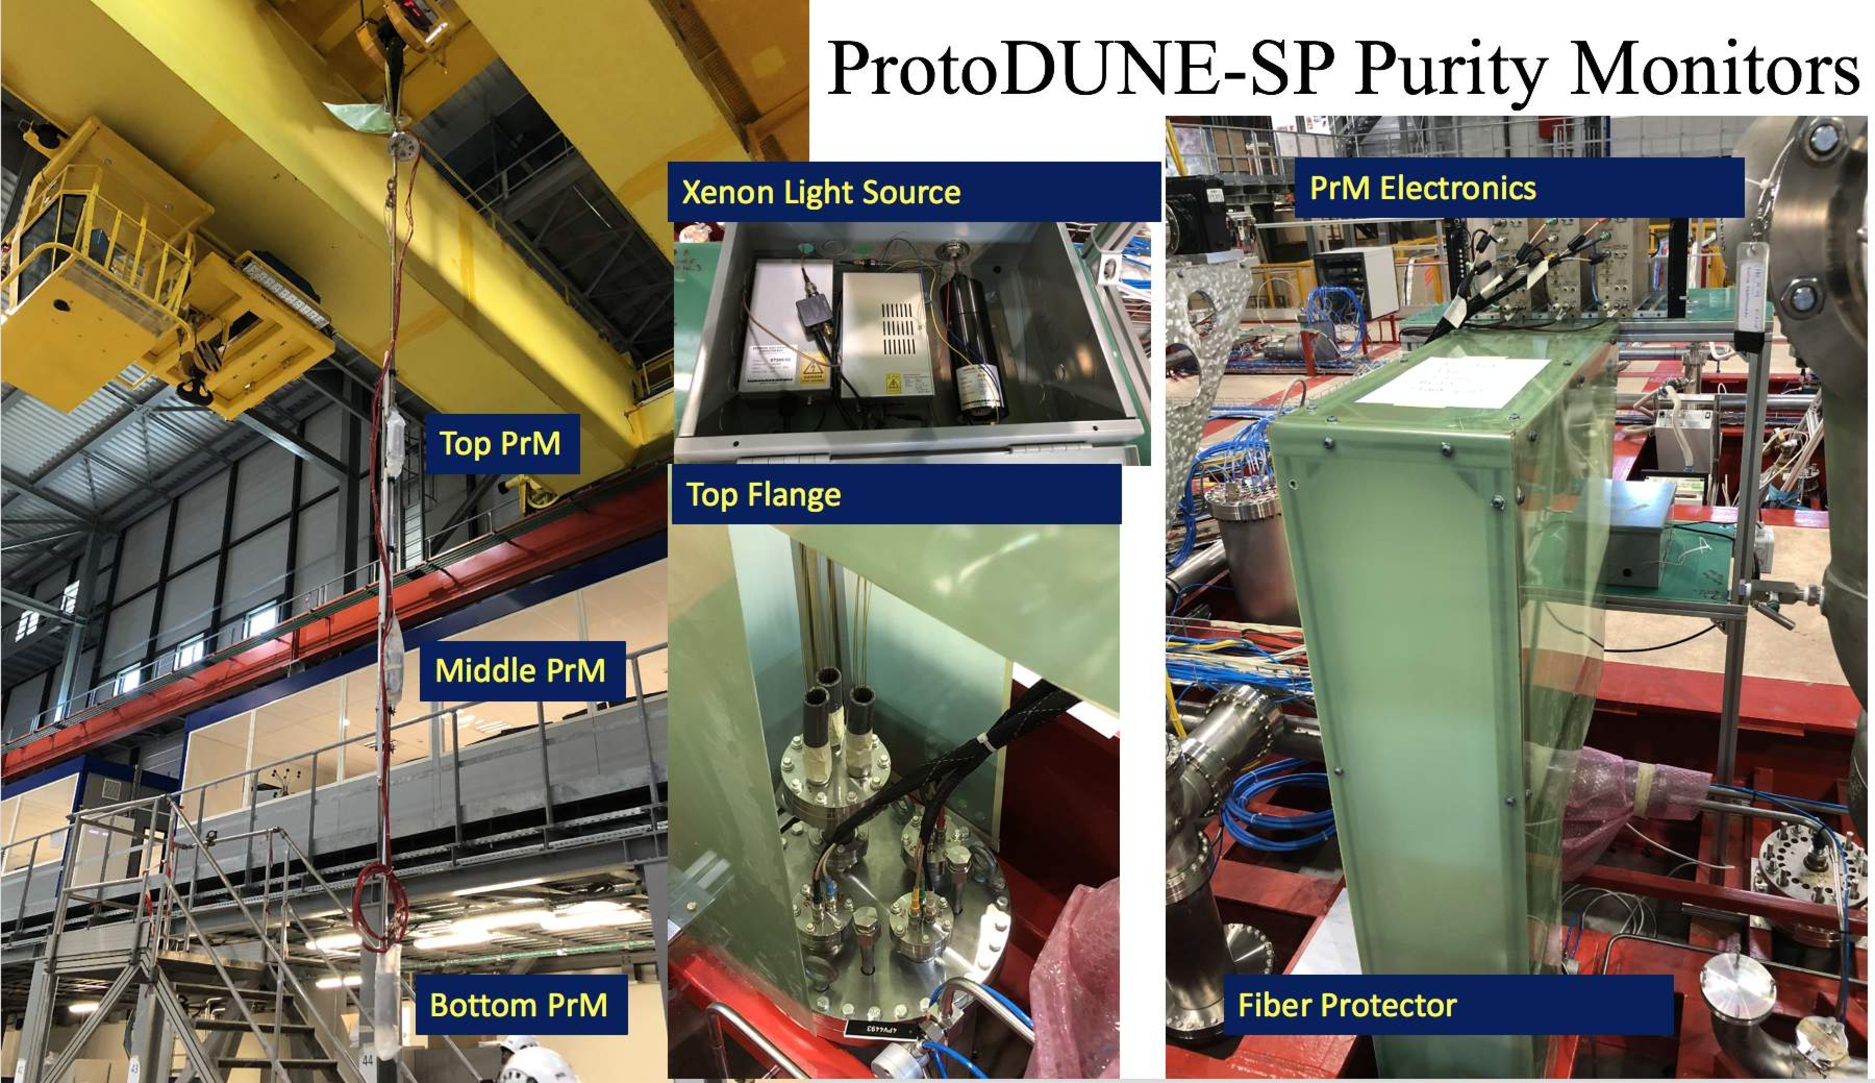
\includegraphics[width=0.9\textwidth]{PrMon_pdsp-PrMAssembly}
\end{dunefigure}


\dword{pdsp} implements three purity monitors. The purity monitors continuously monitored LAr purity during all commissioning, beam test and operation periods of \dword{pdsp}. Figure~\ref{fig-pdsp-prm} shows the \dword{pdsp} data taken using %them 
its three purity monitors from commissioning of \dword{pdsp} starting in September 2018, through the entire beam running, to February 2019.

%to the middle of test beam running, in November 2018. 

\begin{dunefigure}[Measured electron lifetimes in the %four 
three purity monitors at \dword{pdsp}]{fig-pdsp-prm}
  {The measured electron lifetimes as of Feb 2019 in the %four 
  three purity monitors as a function of time in \dword{pdsp}.}
  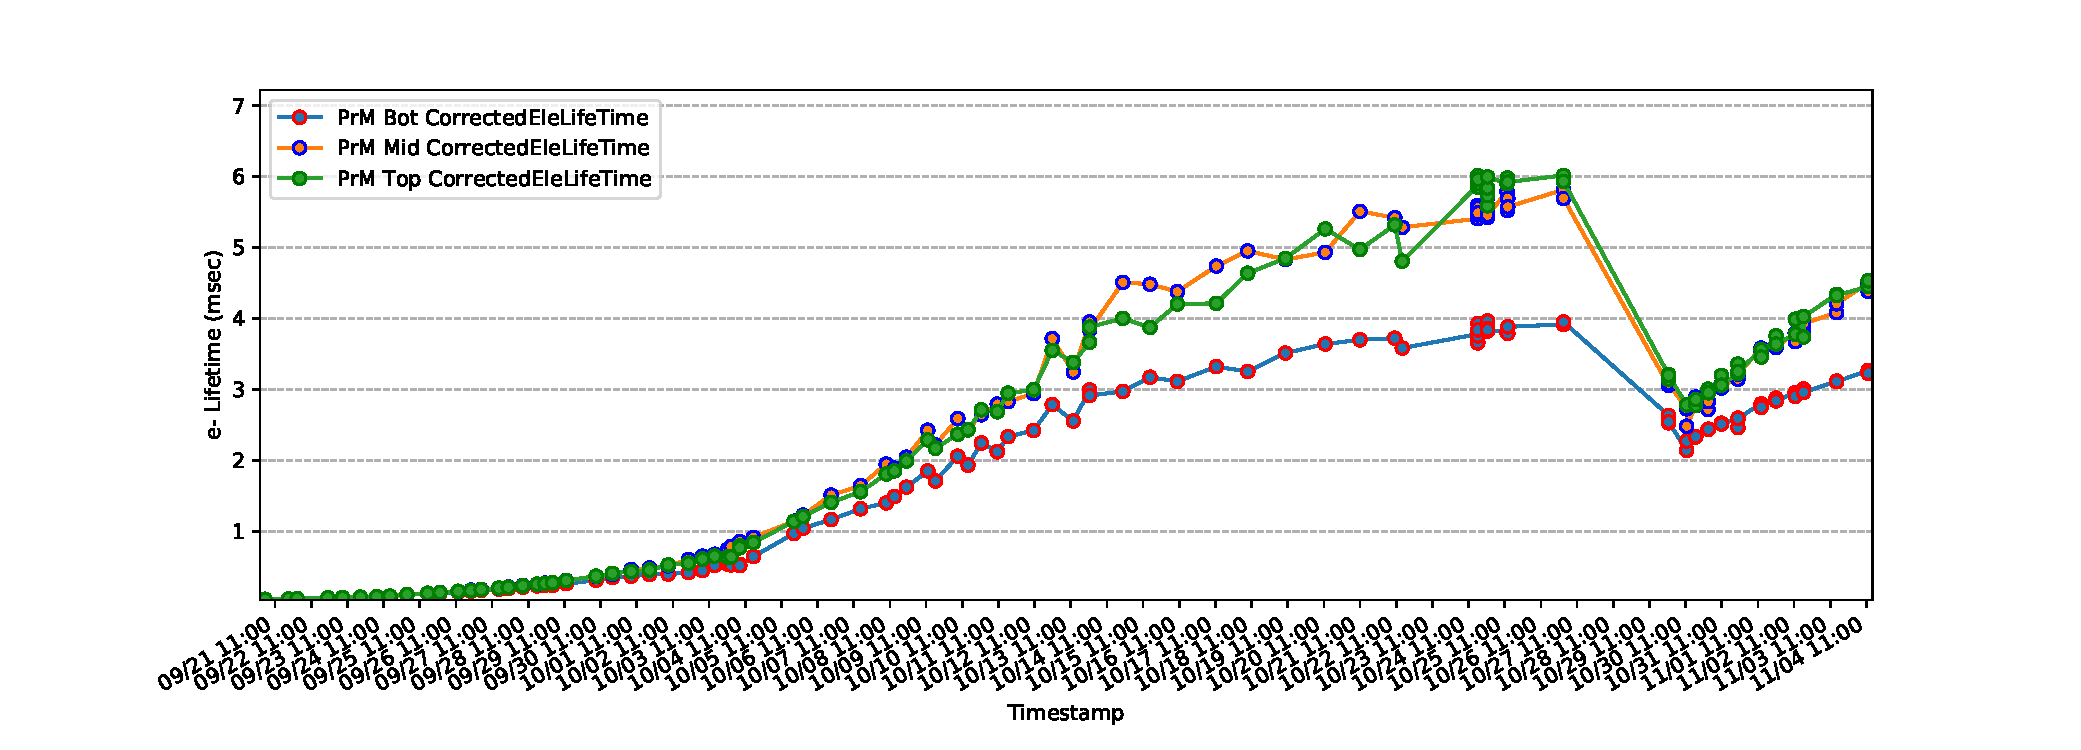
\includegraphics[width=0.9\textwidth]{PrMon_pdsp-PrM.pdf}
\end{dunefigure}



The purity monitor system at \dword{pdsp} measured electron lifetime every hour during commissioning and daily during the beam test. During the commissioning and operation of ProtoDUNE-SP, purity monitors have alerted the experiment solely to serious problems several times. The first time was for filter saturation during LAr filling, and the rest were recirculation pump stoppages, false alarms, and problems from the cryostat-level gauges.  The dips in Figure~\ref{fig-pdsp-prm} show these sudden changes in purity caught by purity monitors. The purity alerts made by purity monitors are crucial to the ProtoDUNE-SP project's success, as they prevented situations which otherwise would have continued unnoticed for some time, with severe consequences to the ability to take any data. Neither the gas analyzers nor the TPC caught these problems in time. 


At \dword{pdsp} (on surface) where we have enough TPC cosmic ray data to measure electron lifetime online, the large fluctuation in the online e-lifetime from TPC data makes it hard to catch the purity change caused by liquid argon re-circulation issue in time. On the other hand, after lower the purity monitor anode high voltage, electron drift time in purity monitors reaches 2.2 ms, the same as the TPC. Furthermore, the purity monitor can take large data sets in a short period of time at the same location, so the statistical error and effects from location dependent uncertainties are smaller in purity monitors compared to TPC. Each purity monitor e-lifetime measurement is based on purity monitor anode-to-cathode signal ratios from 200 UV flashes within 40 seconds at the same location, and the statistic error on the purity monitor e-lifetime is less than 0.03 ms when the purity is 6 ms. With this high sensitivity, purity monitors  caught the purity drops immediately and make the alert to the experiment in time.



%The purity monitor system at \dword{pdsp} measured electron lifetime every hour during commissioning and daily during the beam test. During %commissioning and while running the test beam, 
%this time, it %the purity monitor system at \dword{pdsp} 
%alerted us to serious problems twice, first %. The first time was 
%for filter saturation, and %the second was 
%then that the recirculation pump had stopped. This enabled us to prevent %These alerts were crucial to the success of running the test beam in the \dword{pdsp} project by preventing 
%situations that otherwise could have had serious consequences.



During the commissioning and beam test of \dword{pdsp}, the purity monitors operated with different high voltages to change electron drift time, ranging from \SI{150}{\micro\second} to \SI{3}{\milli\second}. This allowed the \dword{pdsp} purity monitors to measure electron lifetime from \SI{35}{\micro\second} to about \SI{10}{\milli\second} with high precision, a dynamic range greater than \num{300}. %This high-precision electron lifetime measurement was also valuable to the lifetime calibration for  \dword{pdsp}. Because purity monitors have much smaller drift volumes than the \dshort{tpc}, they are less affected by the space charge caused by cosmic rays.
This measurement was also valuable for the \dword{pdsp} lifetime calibration. Because purity monitors have much smaller drift volumes than the \dshort{tpc}, they are less affected by the space charge caused by cosmic rays. 

  A similar purity monitoring system design and operation plan is planned for %are exploited in 
  the \dword{spmod}, with modifications to accommodate the relative positions of the instrumentation port %placement relative to 
  and the purity monitor system, and the %requirements and constraints of 
  different geometric relationships between the \dshort{tpc} and cryostat.




%%%%%%%%%%%%%%%%%%%%%%%%%%%%%%%%%%%%%%%%%%
%\subsubsection{Physics and Simulation}
% Andrew, Jianming





%%%%%%%%%%%%%%%%%%%%%%%%%%%%%%%%%%%%%%%%%
\subsubsection{Purity Monitor Design}
%Laura, Jianming
%WIP IF YOU HAVE MIP PARTICLES LIKE MUONS... NOT TRUE WHEN YOU ARE UNDERGROUND. ALSO, WE HAVE SEEN IN THE 311 THAT MUONS DO NOT DEPOSIT THE EXACT SAME AMOUNT OF ENERGY ACROSS THE TRACK 
%While the \dword{lar} \dshort{tpc} itself can measure the purity of the liquid argon based on the drift electron lifetime, this can only be done once a certain level of purity has been achieved, and until then it may be unclear what the level of purity is and if conditions in the detector are becoming better or worse. 

%The basic design of a purity monitor uses the design in the ICARUS experiment ( Figure~\ref{fig:prm})\cite{Adamowski:2014daa}: a double-gridded ion chamber immersed in the \lar volume.   The purity monitor has four parallel, circular electrodes, a disk holding a photocathode, two grid rings (anode and cathode), and an anode disk. The cathode grid is held at ground potential. The cathode, anode grid, and anode are electrically accessible via modified vacuum grade high-voltage \fdth{}s and separate bias voltages held at each one.   The anode grid and the field shaping rings are connected to the cathode grid by an internal chain of \SI{50}{\mega\ohm} resistors to ensure the uniformity of the \efield{}s in the drift regions. A stainless mesh cylinder is used as a Faraday cage to isolate the purity monitor from external electrostatic background. 

The \dword{spmod} baseline purity monitor design follows that of  the ICARUS experiment (Figure~\ref{fig:prm})\cite{Adamowski:2014daa}.  It consists of a double-gridded ion chamber immersed in the \lar volume with four parallel, circular electrodes, a disk holding a photocathode, two grid rings (anode and cathode), and an anode disk. The cathode grid is held at ground potential. The cathode, anode grid, and anode 
each hold separate bias voltages and are electrically accessible via modified vacuum-grade \dword{hv} \fdth{}s. % and separate bias voltages held at each one.   
The anode grid and the field shaping rings are connected to the cathode grid by an internal chain of \SI{50}{\mega\ohm} resistors to ensure the uniformity of the \efield{}s in the drift regions. A stainless mesh cylinder is used as a Faraday cage to isolate the purity monitor from external electrostatic background. 

The purity monitor measures the electron drift lifetime between its anode and cathode. The purity monitor's UV-illuminated %gold 
photocathode generates the electrons via the photoelectric effect. Because the electron lifetime in \lar is inversely proportional to the electronegative impurity concentration, the fraction of electrons generated at the cathode that arrives at the anode ($Q_A/Q_C$) after the electron drift time $t$ gives a measure of the electron lifetime $\tau$:
%
\( Q_A/Q_C \sim e^{-t/\tau}.\)



\begin{dunefigure}[Schematic diagram of the %basic 
baseline purity monitor design]{fig:prm}
  {Schematic diagram of the basic purity monitor design \cite{Adamowski:2014daa}.}
  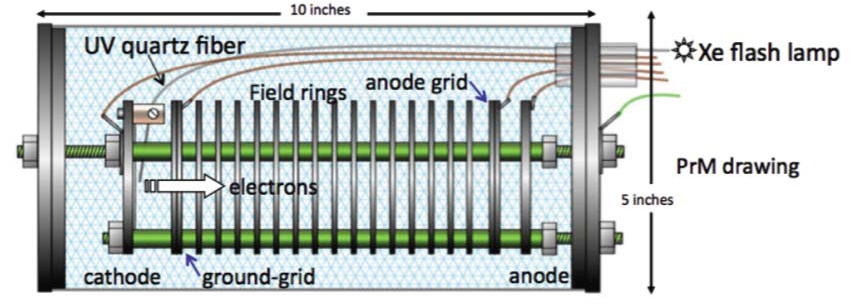
\includegraphics[width=0.9\textwidth]{PrMon_prm.pdf}
\end{dunefigure}


%
%Complete formula would be: Q_A/Q_C = \frac{T_1 \sinh(t_3/2\tau)}{t_3 \sinh(t_1/2\tau)} \exp \left(-\frac{t_2+\frac{t_1+t_3}{2}}{\tau} \right), where$t_1$ is the time it takes the electrons to go from cathode to cathode grid, $t_2$ to go from cathode grid to anode grid, and $t_3$ to go from grid anode to anode. 

%This formula shows 
Once the electron lifetime becomes much larger than the drift time $t$ the purity monitor reaches its sensitivity limit.  For $\tau >> t$, the anode-to-cathode charge ratio becomes $\sim\,1$. Because the drift time is inversely proportional to the \efield, in principle, lowering the %drift 
field should make it possible to measure lifetimes of any length, regardless of the length of the purity monitor.
%means any lifetime can be measured no matter the length of the purity monitor (the lower the field, the lower the drift velocity, i.e., the longer the drift time). 
On the other hand, increasing the voltage will shorten the drift time, allowing measurement of a short lifetime when purity is low. 

The electron lifetime of the purest commercial \lar, after the first filtering and during the filling process, is typically higher than \SI{40}{\micro\second}. However, when the filter starts to saturate, the lifetime decreases to less than \SI{30}{\micro\second}.  To %achieve less 
reduce the energy loss due to impurities,  the \dword{spmod} requires an electron lifetime greater than \SI{10}{\milli\second}.

%According to our experience with \dword{pdsp}, for a 9.5 inch long purity monitor, varying the operational \dword{hv} on the anode from 250 V to 4000 V allows the purity monitors to measure an electron lifetime ranging from 35 $\mu$s to approximately 10 ms with high precision.
Varying the operational \dword{hv} on the anode from \SI{250}{V} to \SI{4000}{V} in the \dword{pdsp}'s \SI{24}{cm} (9.5 inch) long purity monitor allowed us to make the \SI{35}{\micro\second} to \SI{10}{\milli\second} electron lifetime measurements. 
%s ranging from 35 $\mu$s to approximately 10 ms with high precision.
%%% [Deleted this as confusing --- what is ``gas phase'' in single phase detector? --- and not needed. -Glenn] In practice, at very low fields, drifting the electrons all the way up to the anode is difficult, and the discharge in the gas phase limits the anode high voltage to go above 4000 V. \fixme{I read this as "the discharge in the gas phase keeps the voltage in the anode below 4000V." Is that correct? {\em No...}}
%The electron lifetime of the purest commercial \lar, after the first filtering and during the filling process, is typically higher than \SI{40}{\micro\second}. However, when the filter starts to saturate, the lifetime decreases to less than \SI{30}{\micro\second}.  To %achieve less 
%reduce the energy loss due to impurities,  the \dword{spmod} requires an electron lifetime greater than \SI{10}{\milli\second}. Therefore, 
Purity monitors with different lengths (drift distances) are needed to extend the measurable range to below \SI{35}{\micro\second} and above  \SI{10}{\milli\second}.
%Currently, specific sensitivity limits for purity monitors with a drift distance of the order of $\sim$\SI{20}{\centi\meter} are still to be determined in a series of tests. If the required sensitivity is not achieved by these ``short'' purity monitors, longer ones may be developed.

The photocathode that produces the \phel{}s is an aluminum plate coated first with \SI{50}{\angstrom} of titanium followed by \SI{1000}{\angstrom} of gold, and is attached to the cathode disk.
A xenon flash lamp is the light source in the baseline design, although %this could be replaced by 
a more reliable and possibly submersible light source, perhaps LED-driven, could replace this in the future. The UV output of the lamp is quite good, approximately $\lambda=$ \SI{225}{\nano\meter}, which corresponds closely to the work function of gold (\SIrange{4.9}{5.1}{\eV}). 
Several UV quartz fibers carry the xenon UV light into the cryostat to illuminate the %gold 
photocathode.   Another quartz fiber delivers the light into a properly biased photodiode outside the cryostat to provide the trigger signal when the lamp flashes. 



\subsubsection{Electronics, DAQ, and Slow Controls Interfacing}
%Jianming
The purity monitor electronics and \dword{daq} system consist of \dword{fe} electronics, waveform digitizers, and a \dword{daq} PC.  Figure~\ref{fig:cryo-purity-mon-diag} %shows the block diagram of the 
illustrates the system.
%\fixme{block diagram is hard to read - small text and needs more color contrast. Maybe use fewer colors? anne [Carmen] I agree. Contact Jianming to modify colors}

\begin{dunefigure}[Block diagram of the purity monitor system.]{fig:cryo-purity-mon-diag}
  {Block diagram of the purity monitor system.}
  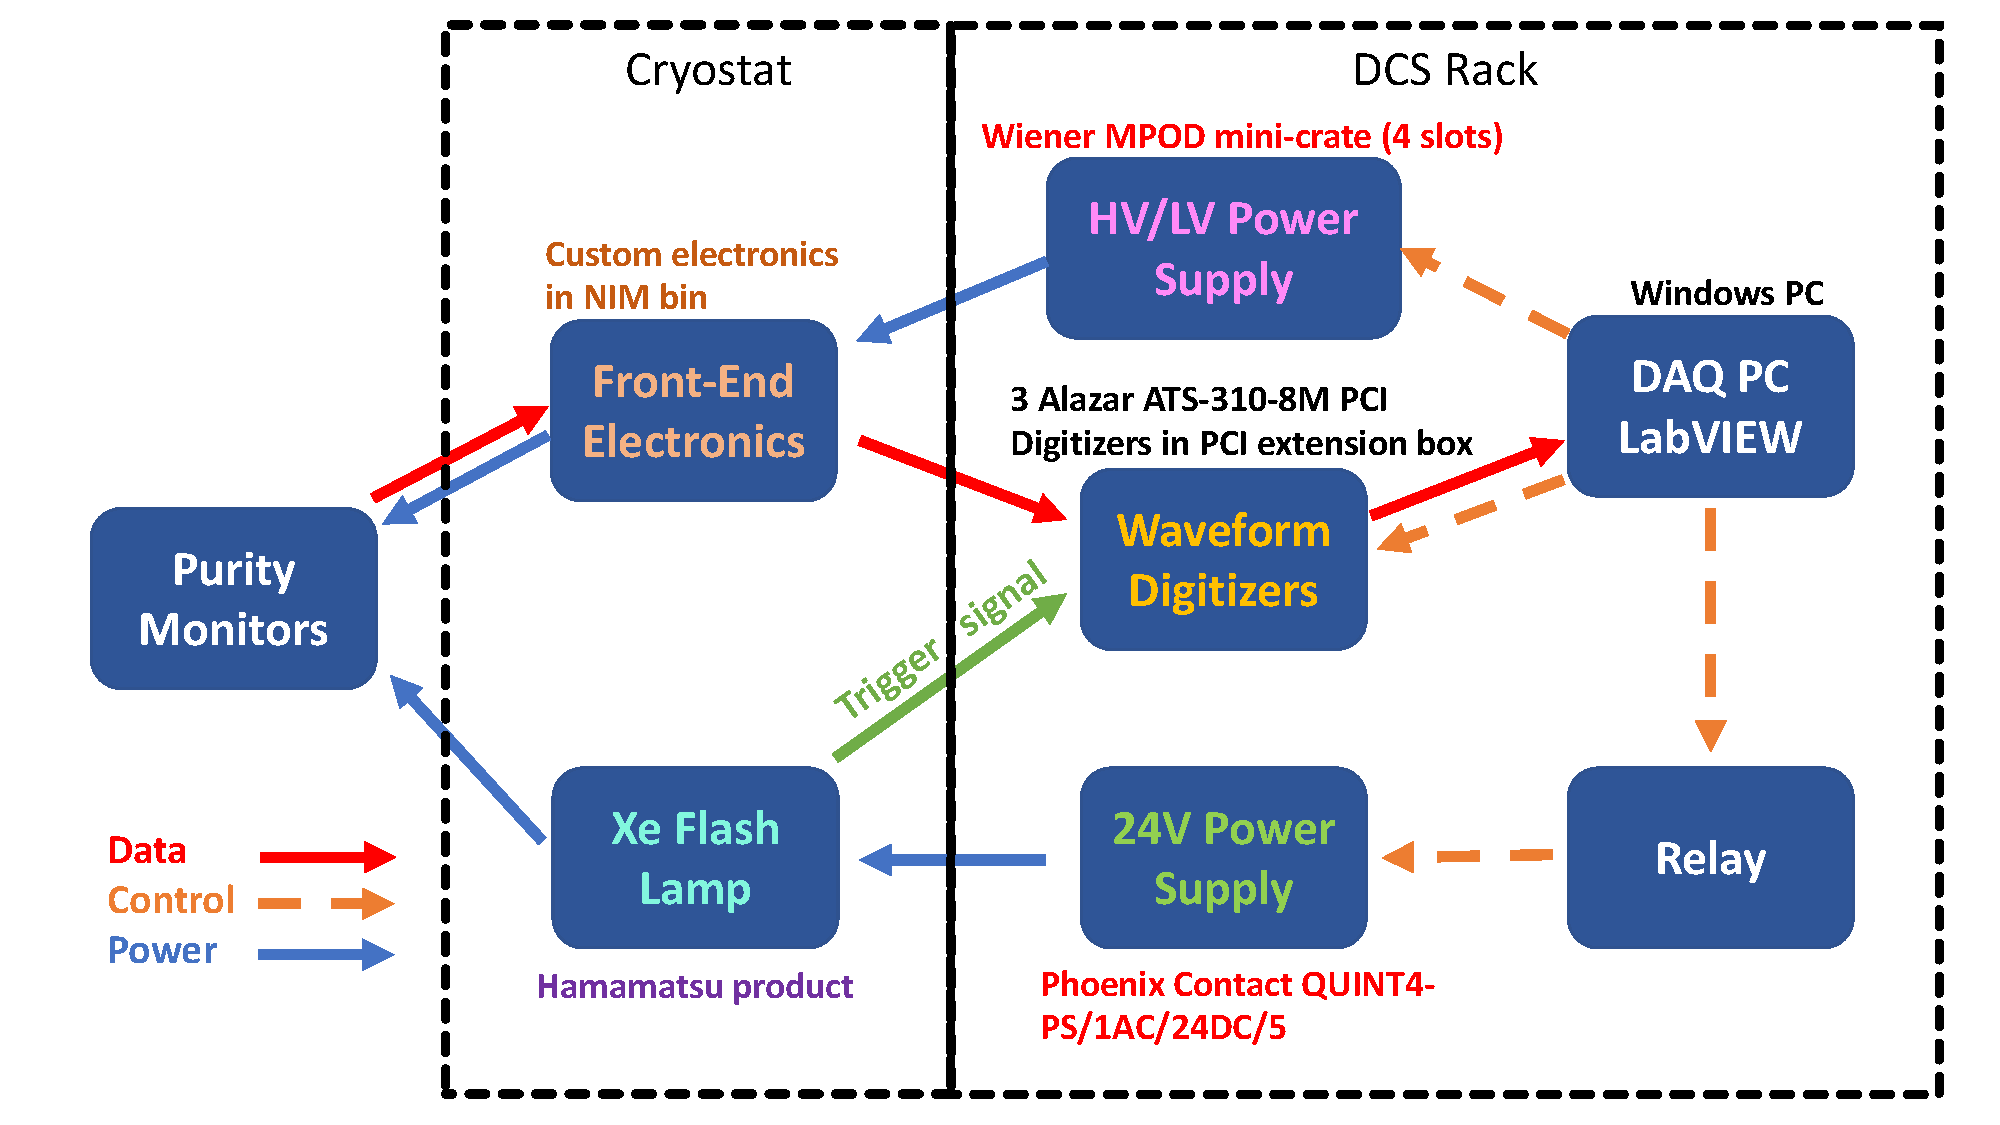
\includegraphics[width=0.95\textwidth]{graphics/PrMon_BlockDiagram_v2.pdf}
\end{dunefigure}


The baseline design of the \dword{fe} electronics follows that used in %is the one used for the purity monitors for 
the \dword{35t}, LAPD, and \microboone. The cathode and anode signals are fed into two charge amplifiers contained within the purity monitor electronics module.
This electronics module includes a \dword{hv} filter circuit and an amplifier circuit, both shielded by copper plates, to allow the signal and \dword{hv} to be carried on the same cable and decoupled inside the purity monitor electronics module. 
A waveform digitizer that interfaces with a \dword{daq} PC records the amplified anode and cathode outputs. 
The signal and \dword{hv} cable shields connect to the grounding points of the cryostat and are separated from the electronic ground with a resistor and a capacitor connected in parallel, mitigating ground loops between the cryostat and the electronics racks. Amplified output is transmitted to an AlazarTech ATS310 waveform digitizer\footnote{AlazarTech ATS310\texttrademark{} - 12 bit, 20 MS/s,  https://www.alazartech.com/Product/ATS310.} containing two input channels, each with 12 bit resolution. Each channel can sample a signal at a rate of \SI{20}{\mega\samples\per\second} to \SI{1}{\kilo\samples\per\second} and store up to \SI{8}{\mega\samples} in memory. One digitizer is used for each purity monitor, and each digitizer interfaces with the \dword{daq} PC across the PCI bus. 
%\fixme{add PCI and labview to glossary? anne}

A custom LabVIEW\footnote{National Instruments, LabVIEW\texttrademark{}, http://www.ni.com/en-us.html} application running on the \dword{daq} PC has two functions: it controls the waveform digitizers and the power supplies, and it monitors the signals and key parameters. The application configures the digitizers to set the sampling rate, the number of waveforms to be stored in memory, the pre-trigger data, and a trigger mode. A signal from a photodiode triggered by the xenon flash lamp is fed directly into the digitizer as an external trigger to initiate data acquisition.  LabVIEW automatically turns on the xenon flash lamp by powering a relay when data taking begins and then turns it off when finished.
The waveforms stored in the digitizers are transferred to the \dword{daq} PC and used to obtain averaged waveforms to reduce the electronic noise in them. % waveforms. 
The baseline  is estimated by averaging the waveform samples prior to the trigger. This baseline is subtracted from the waveforms prior to calculating peak voltages of the cathode and anode signals. %These processes are performed in real time within the application and are then used to estimate the electron lifetime.
The application performs these processes in real time. % within and uses the results to estimate the electron lifetime. 
 The application continuously displays the waveforms and important parameters like measured electron lifetime, peak voltages, and drift time % of electrons 
in the purity monitors, and shows the variation in these parameters over time, thus pointing out %.This allows validating the impurity of the \dword{lar} and seeing 
effects that might otherwise be missed. %may not be spotted at that instant. 
Instead of storing the measured parameters, the waveforms and the digitizer configurations are recorded in binary form for offline analysis.  HV modules\footnote{iseg Spezialelektronik GmbH\texttrademark{} high voltage supply systems, https://iseg-hv.com/en.} in a WIENER MPOD mini crate\footnote{W-IE-NE-R MPOD\texttrademark{} Universal Low and High Voltage Power Supply System, http://www.wiener-d.com/.} supply negative voltages to the cathode and positive voltages to the anode. The LabVIEW application controls and monitors the \dword{hv} systems through an Ethernet interface.
%\fixme{Check the tenses. I see some past tense, quite a lot of present tense, and then some future tense. Make sure tense matches when something occurs, has occurred, or will occur.}

%The xenon flash lamp and the \dword{fe} electronics are installed close to the purity monitor flange, to reduce light loss through the optical fiber and prevent signal loss. Other pieces of equipment are mounted in a rack separate from the cryostat. They distribute power to the xenon flash lamp and the \dword{fe} electronics and collect data from the electronics. The slow control system communicates with the purity monitor \dword{daq} software and controls  the \dword{hv} and \dword{lv} power supplies of the purity monitor system. The optical fiber must be very close to the photocathode (less than \SI{0.5}{\milli\meter}) for efficient \phel extraction, so little interference with the \dword{pds} is expected. The purity monitors could induce noise in the TPC electronics, in particular from the current surge through the xenon lamps when they are flashed.  This source of noise can be controlled by placing the xenon flash lamp inside its own Faraday cage, which allows proper grounding and shielding. According to the operation of purity monitors at \dword{pdsp}, after careful checks of the grounding, this noise is well below noise generated by other sources.
The xenon flash lamp and the \dword{fe} electronics are installed close to the purity monitor flange, to reduce light loss through the optical fiber and prevent signal loss. Other pieces of equipment that distribute power to these items and collect data from the electronics are mounted in a rack separate from the cryostat. The slow control system communicates with the purity monitor \dword{daq} software and controls  the \dword{hv} and \dword{lv} power supplies of the purity monitor system. The optical fiber must be placed within  \SI{0.5}{\milli\meter} of the photocathode for efficient \phel extraction, so little interference with the \dword{pds} is expected. The purity monitors could induce noise in the TPC electronics, in particular via the current surge through a xenon lamp when it is flashed.  This source of noise can be controlled by placing the lamp inside its own Faraday cage with %, which allows 
proper grounding and shielding. %According to the operation of purity monitors 
At \dword{pdsp}, after careful checks of the grounding, this noise has remained well below the noise generated by other sources.

In the \dword{spmod} we can make use of triggering to prevent any potential noise from the purity monitor's flash lamp from affecting TPC and \dword{pds} signals. The LArTPC trigger rate is a few hertz, and each trigger window is one or a few milliseconds. %For a purity monitor's flash lamp,  the flash light 
The pulse from a flash lamp is very short (a microsecond or so, much shorter than the gaps between LArTPC trigger windows). 
% \fixme{is LArTPC trigger window the same as neutrino spill trigger window? Can we just say 'trigger window'? (MISSED WITH TIM) GLENN AND CARMEN TO CHECK - FIXED [Glenn, Sowjanya, Carmen].}
Thus, a LArTPC trigger signal may be sent to a programmable pulse generator, %and the pulse generator then 
which generates a trigger pulse that does not overlap with LArTPC trigger windows. This trigger pulse %will then be 
is then sent to the external trigger port on the flash lamp HV controller so that the lamp flashes between LArTPC trigger windows. In this way, the electronic and light noises from the flash lamp do %will 
not affect %LArTPC 
data taking at all.


%If an unavoidable interference problem is found to exist, then software can be implemented to allow the \dword{daq} to know if and when the purity monitors are running and to veto purity monitor measurements in the event of a \dword{snb} alert or trigger. 


%%%%%%%%%%%%%%%%%%%%%%%%%%%%%%%%%%%%%%%%%%
\subsubsection{Production and Assembly}
\label{sec:PrMon-Production-Assembly}
%Andrew
%Individual purity monitors will be produced and they will be assembled into the string that will be placed into the \dword{detmodule} cryostat following the methodology developed for \dword{protodune}.  Each monitor is fabricated, assembled, and then tested in a smaller test stand.  After confirming that each purity monitor operates at the required level, all monitors are assembled into strings using support tubes that mount the system inside the cryostat with three purity monitors grouped together to form one string, as shown in Figure~\ref{fig:PrMon-SystemString}.

The \dword{cisc} consortium will produce the individual purity monitors, test them in a test stand, and confirm that each monitor operates at the required level before assembling them into the strings of three monitors each that will be mounted in the \dword{detmodule} cryostat using support tubes. The assembly process will follow the methodology developed for \dword{protodune}.

%The assembly of the individual purity monitors into the string would follow the steps laid out in the first 5 panels of Fig.~\ref{fig:PrMon-Assembly}.

% Anne and Tim decided to remove this figure 1/17 - content-free and no ref to it.
%\begin{dunefigure}[Design of the purity monitor string of three monitors.]{fig:PrMon-SystemString}
%  {Design of the purity monitor string of three monitors.}
%  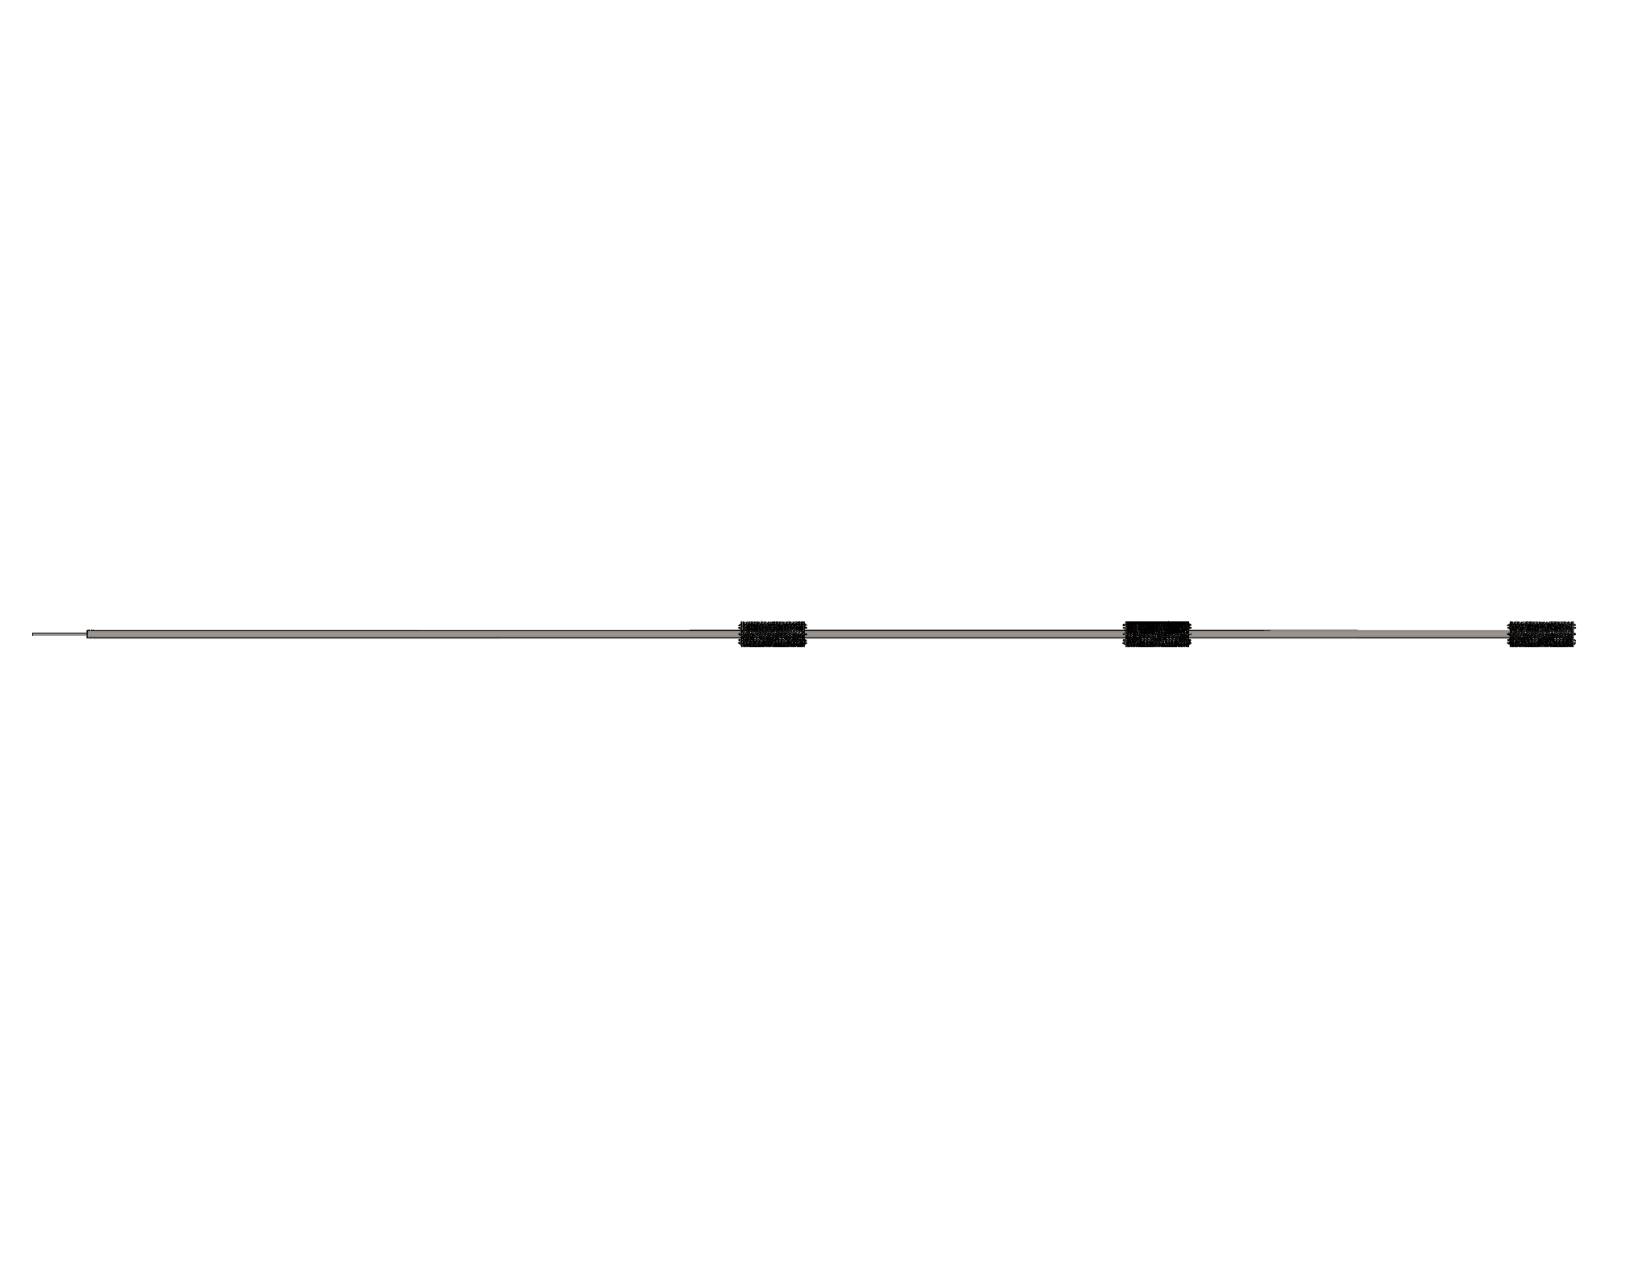
\includegraphics[width=0.9\textwidth]{PrMon-SystemString.pdf}
%\end{dunefigure}


%\begin{dunefigure}[Purity Monitor String Assembly]{fig:PrMon-Assembly}
%  {Assembly sequence of the purity monitors.}
%  \includegraphics[width=\textwidth]{PrMon-Assembly.pdf}
%\end{dunefigure}



A short version of the %assembly
string
%\fixme{string?}
with all purity monitors will be tested in the \lar test facility. The full string will be assembled and shipped to \surf. 
 A vacuum test in a long vacuum tube will be performed on-site before inserting the full assembly into the \dword{spmod} cryostat. 

%not clear if we want to ship the 12 meter assembly or assemble onsite yet.
%Each monitor is assembled as the string is built from the top down, and in the end %there would be 
%three individual purity monitors %hanging 
%hang from a single string.  The assembly of the string concludes once the purity monitors are each in %place, but with the Faraday cages removed and the \dword{hv} cables and optical fibers yet to be run.  
%This full string assembly is then %would then be 
%shipped to the \dword{fd} site for installation into the cryostat. // a shorter version need to be tested in the LAr testing facility


%%%%%%%%%%%%%%%%%%%%%%%%%%%%%%%
\subsection{Thermometers}
\label{sec:fdsp-cryo-therm}
As discussed in section \ref{sec:fdgen-cryo-cfd}, a detailed \threed temperature map is important %in 
for monitoring %whether the cryogenic system is functioning correctly and the \lar is uniform.
the cryogenic system for correct functioning and the \lar for uniformity.
Given the complexity and size of purity monitors, they can only be installed on the sides of the cryostat to provide a local measurement of
\lar purity. %While a direct measurement of the LAr purity across the entire cryostat is not viable, a sufficiently detailed \threed temperature map can predict LAr purity using \dword{cfd} simulations. The vertical coordinate is especially important because it will be closely related to LAr recirculation and uniformity. 
A direct measurement of the \lar purity across the entire cryostat is not feasible, but a sufficiently detailed \threed temperature map based on \dword{cfd} simulations can predict it. The vertical coordinate is especially important because it will relate closely to the 
\lar recirculation and uniformity. 

The baseline sensor distribution and the cryostat ports used to extract cables (with indication of number of cables per port) are shown in Figure~\ref{fig:cisc-tsensor-map}. The baseline distribution will evolve as more information becomes available (precise \dword{cfd} simulations, better understanding of \dword{dss} ports, installation interfaces with other groups), but the baseline suffices to establish the overall strategy.

\begin{dunefigure}[Distribution of temperature sensors inside the cryostat]{fig:cisc-tsensor-map}
  {Distribution of temperature sensors inside the cryostat}
  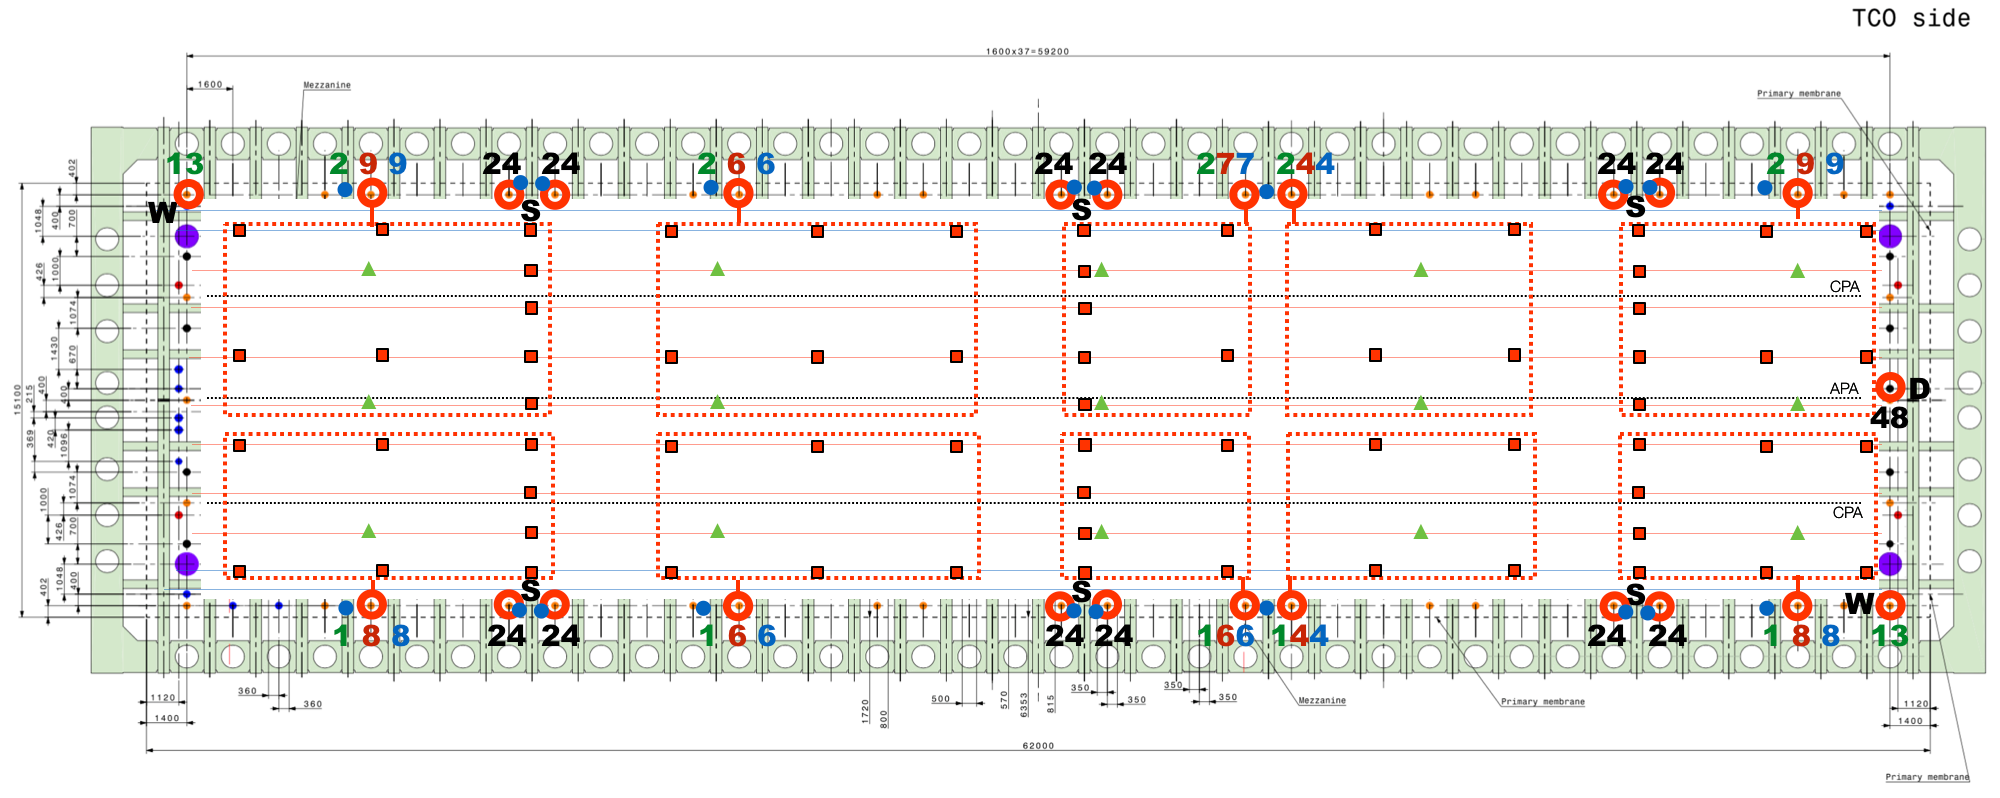
\includegraphics[width=0.95\textwidth]{cisc_tsensor_map_crop.png}
  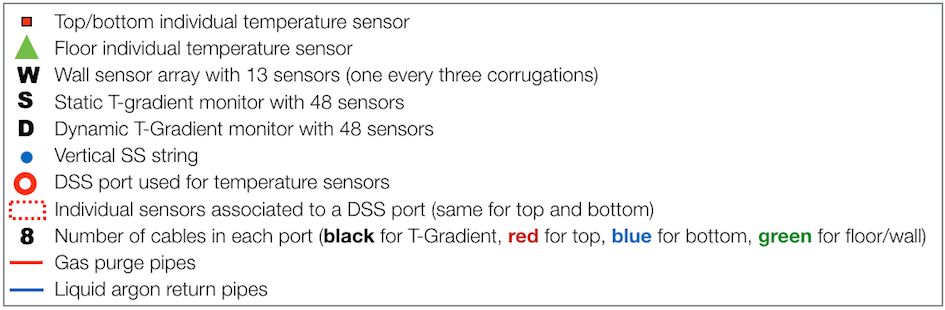
\includegraphics[width=0.85\textwidth]{cisc_tsensor_map_legend.png}
\end{dunefigure}
%\fixme{legend is hard to read in figure (anne)}

High-precision temperature sensors will be distributed near the TPC walls in two ways:
(1) forming high density (\(>2\) sensors/\si{m}) vertical arrays %(the so-
(called T-gradient monitors) and (2) in coarser ($\sim$ 1 sensor/\SI{5}{m}) 2D arrays %(the so-
(called individual sensors) at the top and bottom of the \dword{detmodule}, where it is most crucial to know the temperature.%\fixme{[Carmen] Check Anne's modification} %which are the most delicate regions. 

% Somehow the text below got changed such that the distinction between installation and calibration got really muddled.  Rewritten paragraph added below.
% Temperature variations inside the cryostat should be very small ($\SI{0.02}{K}$; see Figure~\ref{fig:cfd-example}), 
% so sensors must be cross-calibrated to more than $\SI{0.005}{K}$. Most sensors will be calibrated in the laboratory before installation. 
% (Installation is described in section \ref{sec:fdgen-slow-cryo-install-th}.) Where available space is restricted, the only viable way to install sensors is on the long sides of the detector
% % (behind the APAs for SP, and behind the lateral FC end-walls for DP) 
% and the top and bottom of the cryostat.  
% Given the precision required and the unknown longevity of the sensors -- possibly requiring another  calibration after some time -- a complementary method
% will be used for T-gradient monitors behind the front end-walls.
% \fixme{why here? and is it end wall of cryostat or field cage? No hyphenated end-wall; pls fix. GLENN AND CARMEN TO CHECK}
% % at least for the SP detector.
% In areas with sufficient space for a movable system, %this 
% another calibration method, described in section \ref{sec:fdgen-slow-cryo-dynamic-therm}, can be used to cross calibrate
% the temperature sensors in situ.% This calibration method is . 

\fixme{Rewritten paragraph below based on text from Anselmo [Glenn]}

Temperature variations inside the cryostat should be very small ($\SI{0.02}{K}$; see Figure~\ref{fig:cfd-example}),
so sensors must be cross-calibrated to better than $\SI{0.005}{K}$. Most sensors will be calibrated in the laboratory before installation.
(Installation is described in section \ref{sec:fdgen-slow-cryo-install-th}.)
Calibration before installation is the only option for sensors installed on the long sides of the detector and the top and bottom of the cryostat, where space is limited.
Given the precision required and the unknown longevity of the sensors -- possibly requiring another  calibration after some time -- an additional method
will be used for T-gradient monitors installed on the short ends of the detector in the space between the field cage end walls and the cryostat walls. There is sufficient space in this area for a movable system, which can be used to cross calibrate
the temperature sensors {\em in situ}, as described in \ref{sec:fdgen-slow-cryo-dynamic-therm}.

The baseline design for all thermometer systems have three elements in
common: sensors, cables, and readout system. We plan to use Lake Shore
PT100-series\footnote{Lake Shore Cryotronics\texttrademark{} platinum RTD series,
  \url{https://www.lakeshore.com/}.} %products/cryogenic-temperature-sensors/platinum-rtds/models/Pages/Overview.aspx}.} 
platinum sensors with \SI{100}{\ohm} resistance %are used 
because in
the temperature range \SIrange{83}{92}{K} %these particular sensors
they 
show high reproducibility of $\sim\SI{5}{mK}$ and absolute temperature
accuracy of \SI{100}{mK}.  Using a four-wire readout greatly reduces
issues related to lead resistance, any parasitic resistances,
connections through the flange, and general electromagnetic noise
pick-up. Lakeshore PT102 sensors (see
Figure~\ref{fig:sensor-support}-Right) were used in the \dword{35t} prototype
and \dword{pdsp}, % detector, 
giving excellent results. For the inner
readout cables, a custom cable made by Axon\footnote{Axon\texttrademark{} Cable, \url{http://www.axon-cable.com}.}
is the baseline. It
consists of four teflon-jacketed copper wires (AWG28), forming two
twisted pairs, with a metallic external shield and an outer teflon
jacket.
%Further details are given in Fig.~\ref{fig:sensor_cable}-Right. 
The readout system is described in section \ref{sec:fdgen-slow-cryo-therm-readout}.

%As shown in Fig.~\ref{fig:sensor_cable}, the PT102 sensor has a length of \SI{21}{mm}, which can easily be accommodated in the \dword{dune} T-gradient monitors. 

%\begin{dunefigure}[\dword{dune} baseline choices for sensor and cable]{fig:sensor_cable}
%  {\dword{dune} baseline choices for sensor and cable. Left: Schematic diagram of the PT102 sensor from the Lakeshore company. Right: Schematic diagram and properties of the four wires cable from the
%  Axon company}
%  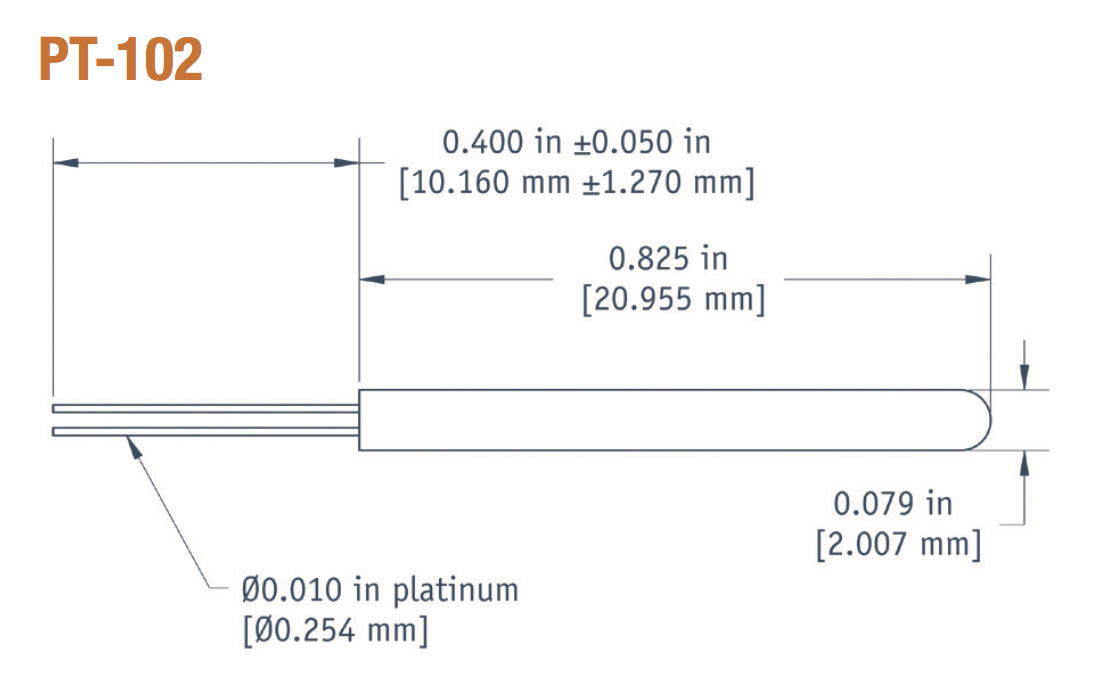
\includegraphics[width=0.4\textwidth]{cisc_pt102.png}
%  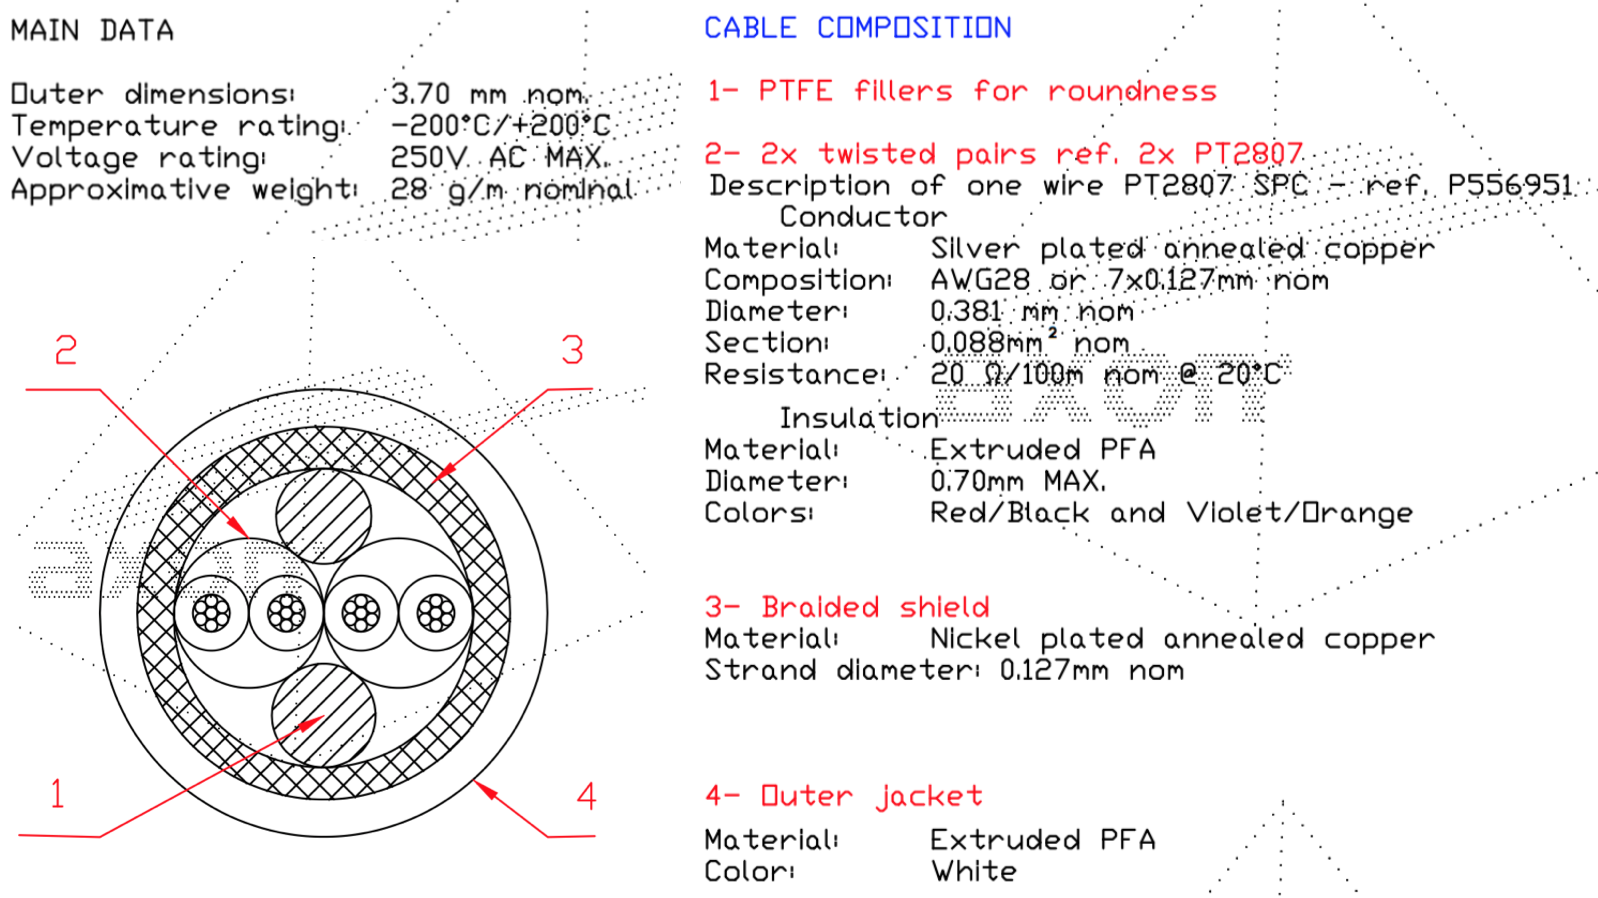
\includegraphics[width=0.55\textwidth]{cisc_TAxonCable.png}
%\end{dunefigure}

Another set of lower-precision sensors epoxied into the bottom membrane of the cryostat will monitor  the cryostat filling in the initial stage.   
Finally, the inner walls and roof of the cryostat will have the same types of sensors to monitor the temperature during cooldown and filling (W sensors in Figure~\ref{fig:cisc-tsensor-map}).
 
% \fixme{Remove references to DP -- done}
 
%except for the membrane sensors that may come from Minco.

% % % %
\subsubsection{Static T-gradient monitors}
\label{sec:fdgen-slow-cryo-static-therm}

Several vertical arrays of high-precision temperature sensors cross-calibrated in the laboratory will be installed behind the \dword{apa}s.  
% near the lateral walls.
%(behind the APAs for SP and behind the lateral FC end-walls for DP). 
%For the SP detector, since the electric potential is zero behind the APAs, no electric field shielding is required, simplifying enormously the mechanical design.
%\footnote{This does not apply for the DP detector, for which the proper shielding must be provided.} 
The baseline design assumes six arrays with \num{48} sensors each. Spacing between sensors
is \SI{20}{cm} at the top and bottom and \SI{40}{cm} in the middle area. This configuration is similar to the one used in \dword{pdsp} but with nearly double the spacing. 
As shown in Figure~\ref{fig:cisc-cfd-valid} a configuration with \num{48} sensors was appropriate in \dword{pdsp}, as it should be in the \dword{spmod} where the expected total gradient is no larger than in \dword{pdsp} (see Figure~\ref{fig:cfd-example}). 

\begin{dunefigure}[Temperature sensor resolution and reproducibility]{fig:Trepro}{
 Left:   Temperature offset between two sensors as a function of time for four independent immersions in LAr. The reproducibility of those sensors, defined as the RMS of the mean offset in the flat region, is $\sim\,\SI{1}{mK}$,
    The resolution for individual measurements, defined as the RMS of one offset in the flat region, is better than \SI{0.5}{mK}. Right: Difference between the mean offset obtained with two independent calibration methods for the 51 calibrated sensors. The standard deviation of this distribution is interpreted as precision of the calibration.}
  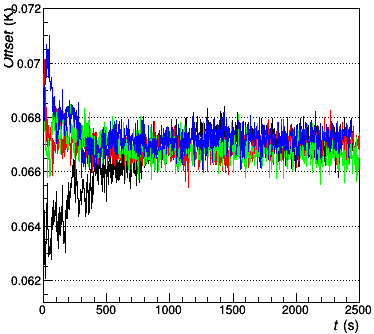
\includegraphics[height=0.44\textwidth]{cisc_tsensor_calib.png}%
  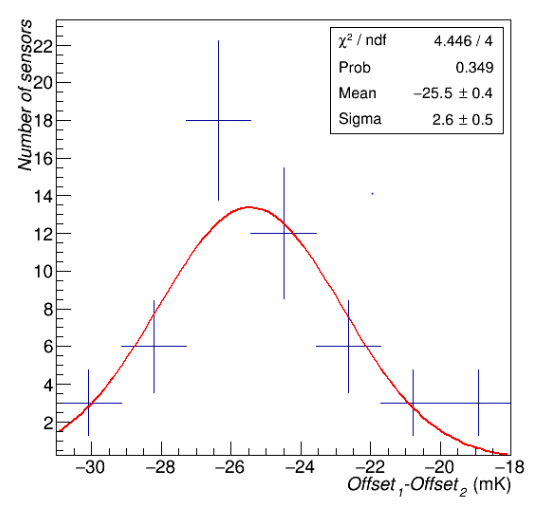
\includegraphics[height=0.45\textwidth]{cisc_tsensor_calib2.png}%
\end{dunefigure}

Sensors will be cross-calibrated in the laboratory using a controlled environment and a high-precision readout system, described in subsection \ref{sec:fdgen-slow-cryo-therm-readout}.
%Although the calibration procedure will certainly improve, the one currently used for \dword{pdsp} is descrived here.
%Four sensors are placed as close as possible (such that identical temperature can be assumed for all of them) inside a small cylindrical aluminum capsule,
%which protects the sensors from thermal shocks and helps in minimizing convection.
%One of the sensors acts as reference while the other three are the ones being calibrated. Five independent calibrations
%are performed for each set of three sensors, such that the reproducibility of each sensor can be computed. For each calibration 
%the capsule is introduced in a PLA box of size \(9.5\times9.5\times\SI{19}{cm^3}\), with two concentrical independent volumes of LAr
%and sourounded by a polystyrene box with \SI{15}{cm} thick walls. A small quantity of LAr is used to slowly
%cooldown the capsule to $\sim\SI{90}{K}$, avoiding thermal shocks that could dammage the sensors.
%Then the capsule is covered by LAr such that it penetrates
%inside fully covering the sensors. Once the temperature stabilizes to the 1-\SI{2}{mK} level (after 5-15 minutes) measurements are taken. Then the capsule is taken out from LAr
%and kept at room temperature until it reaches \SI{200}{K}. As mentioned above, this procedure is repeated five times, before going to the next set of three sensors.  
The accuracy of the calibration for \dword{pdsp} was estimated to be $\SI{2.6}{mK}$, as shown in Figure~\ref{fig:Trepro}. Preliminary results for the analysis of \dword{pdsp} static T-gradient monitor data are shown in Figure~\ref{fig:pd_static_t_results}. The temperature profile has been computed using both the laboratory calibration and the so-called \textit{in-situ pump-off calibration}, which consists %in 
of estimating the offsets between sensors assuming the temperature of \lar in the cryostat is homogeneous when the re-circulation pumps are off (the validity of this method is demonstrated in Section~\ref{sec:fdgen-slow-cryo-dynamic-therm}).  
The RMS of the difference between both methods is $\SI{4.6}{mK}$, slightly larger than the value quoted above for the accuracy of the laboratory calibration, due to the presence of few outliers (under investigation) and to the imperfect assumption of homogeneous temperature when pumps are off (see Figure~\ref{fig:dynamic_t_pumps-off}).  

\begin{dunefigure}[ProtoDUNE-SP Static T-gradient results]{fig:pd_static_t_results}{
 Left: Temperature profile as measured by the Static T-gradient monitor for two different calibration methods. Right: Distribution of the difference between both methods.}
  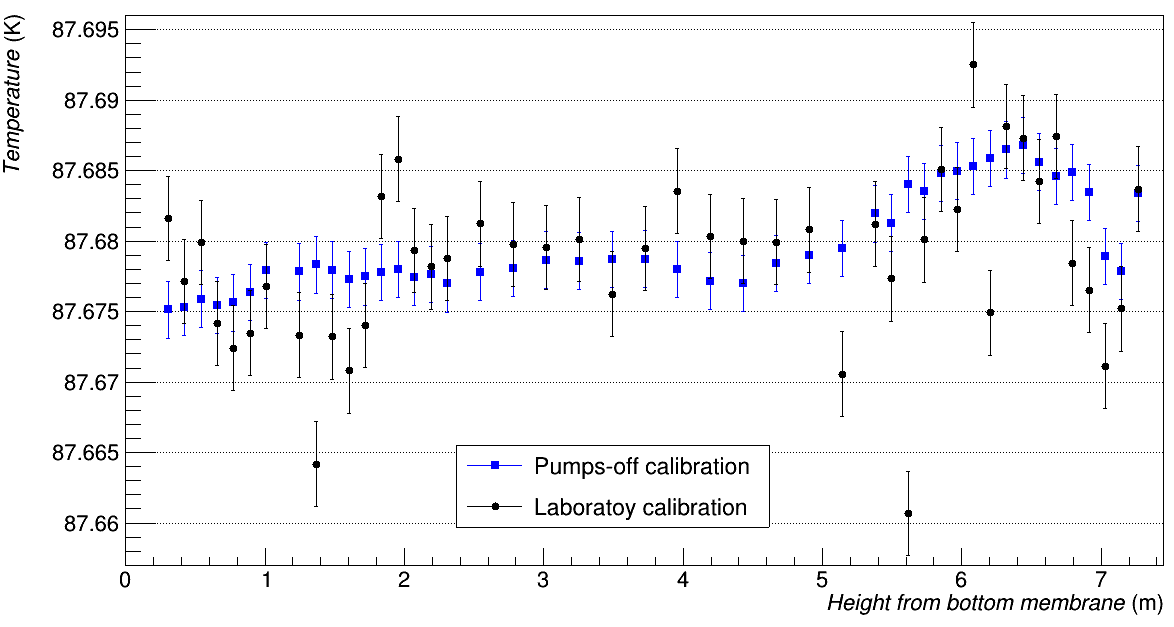
\includegraphics[height=0.34\textwidth]{cisc_static_t_profiles.png}%
  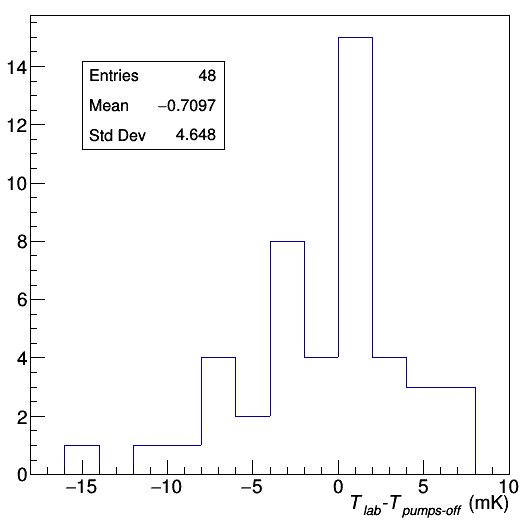
\includegraphics[height=0.34\textwidth]{cisc_static_t_calib_diff.png}%
\end{dunefigure}


\begin{dunefigure}[Conceptual design of the static T-gradient monitor]
{fig:cisc-static-tgradient}
  {Conceptual design of the static T-gradient monitor.}
  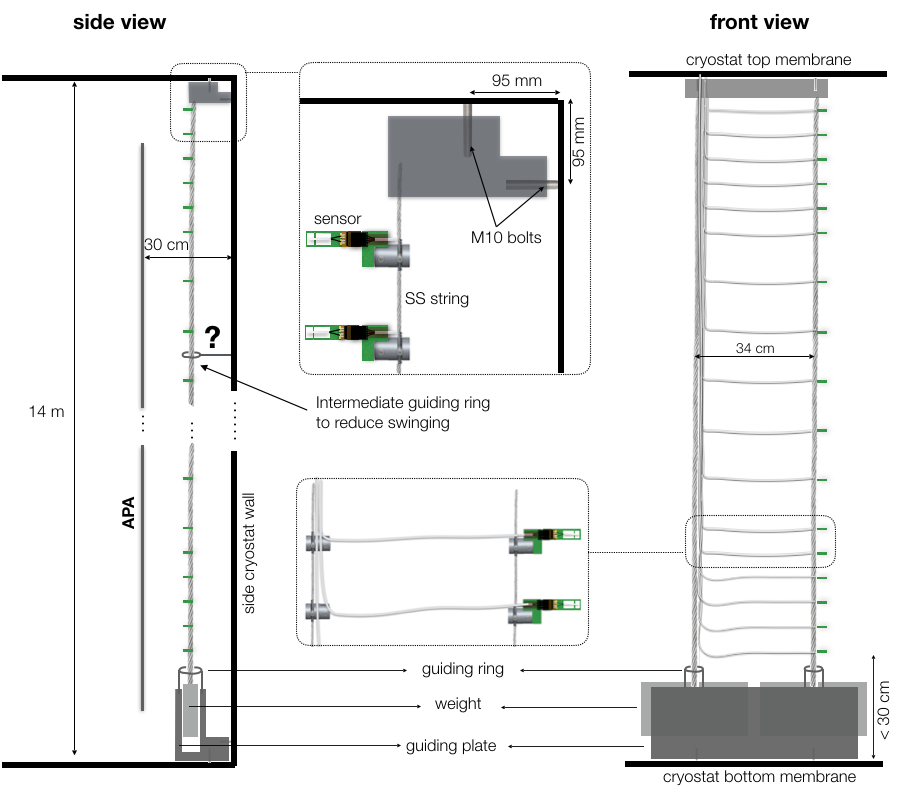
\includegraphics[width=0.8\textwidth]{cisc_static_tgradient.png}
\end{dunefigure}

Figure~\ref{fig:cisc-static-tgradient} shows the baseline mechanical design of
the static T-gradient monitor. Two stainless steel strings are anchored at the top and bottom corners of the cryostat
using the available M10 bolts (see Figure~\ref{fig:sensor-support}, left). One string routes the cables while the other,
separated from the first by \SI{340}{mm},  supports the temperature sensors.
Given the height of the cryostat, an intermediate anchoring point is needed to reduce swinging. This is still under discussion. To account for shrinkage in the strings under cryogenic conditions and to guarantee that the same tension is always applied, a weight is hung at the bottom of the strings. A guiding system made of stainless steel and anchored by four M10 bolts at the bottom keeps the weight confined in space. A prototype is being built at \dfirst{ific}, where the full system will be mounted using two dummy cryostat corners. We are also considering an alternative design with carbon fiber strings.  
%\fixme{please remake ific glossary term and send it to me so I can put it in master copy. 10 Apr. Anne}


Figure~\ref{fig:sensor-support}, right shows the baseline design of the ($52\times \SI{15}{mm^2}$) 
PCB support for temperature sensors with an IDC-4 male connector. %It is . 

A narrower connector (with two rows of two pins each) is being studied. This alternative design would reduce the width of the PCB assembly and allow more sensors to be calibrated simultaneously. Each four-wire cable from the sensor to the flange will have an IDC-4 female connector on the sensor end; the flange end of the cable will be soldered or crimped to the appropriate connector, whose type and number of pins  depend on the final design of the \dword{dss} ports that will be used to extract the cables. SUBD-25 connectors were used in \dword{pdsp}.

\begin{dunefigure}[Cryostat bolts and temperature sensor support]{fig:sensor-support}
  {Left: bolts at the bottom corner of the cryostat. Right: Lakeshore PT102 sensor mounted on a PCB with an IDC-4 connector.}
  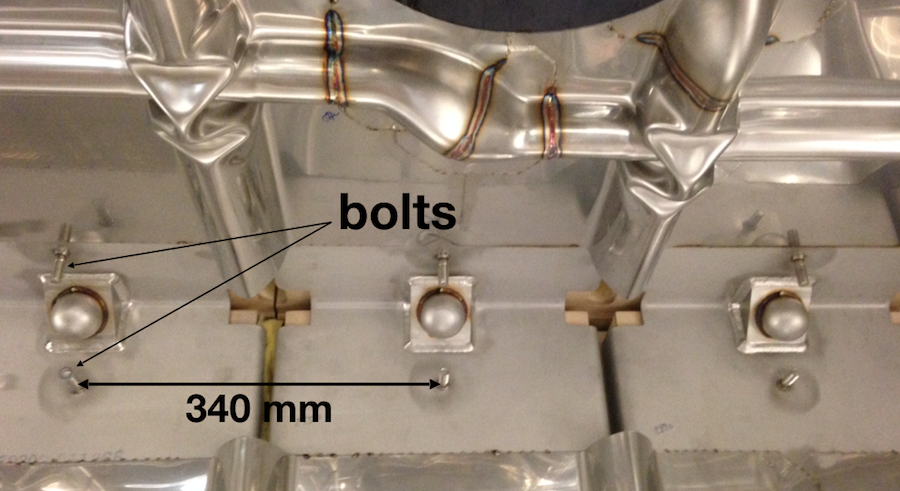
\includegraphics[height=0.2\textwidth]{cisc_cryostat_bolts.png}%
    \hspace{1cm}%
  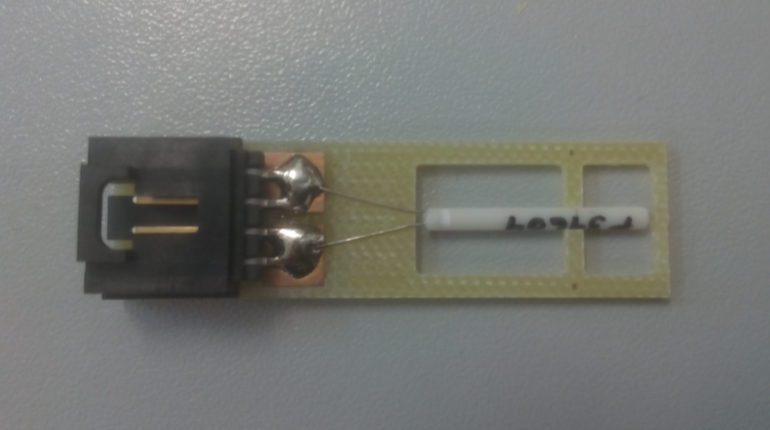
\includegraphics[height=0.2\textwidth]{cisc_tsensor.png}%
\end{dunefigure}




% \begin{dunetable}
% [Static t-gradient parameters]
% {p{0.2\textwidth}p{0.1\textwidth}p{0.6\textwidth}}
% {tab:fdgen-cisc-static-tgradient}
% {Parameters for the Static T-gradient monitor}   
% Parameter            & {\bf value} & {\bf comment} \\ \toprowrule
% \# sensors	         &     48      &       \\ \toprowrule
% sensor spacing       &    20/40 cm & 20 at top and bottom and 40 in the mid area  \\ \toprowrule
% cable diameter       &   3.5 mm    &       \\ \toprowrule
% cable weight         &   28 g/m    &       \\ \toprowrule
% cable-string weight  &   13 Kg     &  10 Kg for the cable, 1.3 Kg for the SS string and 1.7 kg for the cable supports      \\ \toprowrule
% sensor-string weight &   3.3 Kg     & 1.3 Kg for the SS string, 1.7 kg for the cable supports and 300 g for the sensors     \\ \toprowrule
% \end{dunetable}

%Table \ref{tab:fdgen-cisc-static-tgradient} summarizes key properties of the static T-gradient monitor.

% % % %
\subsubsection{Dynamic T-gradient monitors}
\label{sec:fdgen-slow-cryo-dynamic-therm}
% What I was thinking about is to have 3 sensors per meter. 4 would be even better and have 1.35 m range of motion. The goal is to have 4 sensor overlap. In this case, we would be quite safe against sensor failure.
% If we are to populate 14 m with 3 sensors per meter, that would be 42 sensors. In addition, we should increase frequency at the top or bottom.

%The dynamic temperature monitor is a vertical array of high precision temperature sensors to measure the vertical temperature gradient within a few mK. The design of the system is driven by the following:
%\begin{itemize}
%\item
%Uncertainties in the measured vertical temperature profile must be less than a few mK over the entire detector height to monitor LAr purity and provide useful feedback on the efficiency of cryogenic recirculation and purification.
%\item
%Simulations of cryogenic recirculation predict very slow changes in temperature at meter scale except at the bottom and top of the cryostat. Thus, sensors will be placed every \SI{50}{cm} along the detector height with more sensors in the first \SI{50}{cm}, closest to the bottom of the cryostat, and the last \SI{50}{cm}, closest to the top of the cryostat, where spacing between sensors is reduced to \SI{10}{cm}.
% \end{itemize}

% ANSELMO: Paragraph below removed, since it is substituted by the one by Jelena

%The dynamic T-gradient monitor is a vertical array of high precision temperature sensors to measure the vertical temperature gradient within a few mK. 
%To address concerns about potential differences in sensor readings before and after installation in the \dword{dune} \dword{fd}, the dynamic T-gradient monitor allows cross-calibration of sensors {\em in situ}. Namely, the system can move vertically while installed in the \dword{fd} such that a given sensor can be placed at the nominal position of its neighbor, and the temperature offset between them can be computed assuming the temperature at that location did not change during the movement. 

% \fixme{New paragraph from Jelena below. (2019-01-11)}

 To address concerns about potential differences in sensor readings prior to and after installation in a \dword{detmodule}, and potential drifts over the lifetime of the %detector 
 module that may affect accuracy of the vertical temperature gradient measurement, % in a \dword{detmodule}, 
 a dynamic temperature monitor allows cross-calibration of sensor readings %{\em in situ}. 
 in situ.
Namely, this T-gradient monitor is motorized, allowing vertical motion of the temperature sensor array %in vertical direction while installed 
in the \dword{detmodule}, %. This ability enables 
enabling precise cross-calibration between the sensors, %{\em in situ
as illustrated in Figure~\ref{fig:sensor-cross-calibration}.  

The procedure for cross-calibrations is the following: in step 1, the temperature reading  of all sensors is taken at the home (lowest) position of the carrier rod. In  step 2, the stepper motor moves the carrier rod up \SI{25}{cm}. Since the sensors along the entire  carrier rod are positioned \SI{25}{cm} apart, when the system is moved up \SI{25}{cm}, each sensor is positioned at the height that was occupied by another sensor in step 1. Then a second temperature reading is taken. In this manner, except for the lowest position two temperature measurements are taken at each location with %two 
different sensors. Assuming that the temperature at each location is stable over the few minutes required to make the measurements, %the 
any difference in the temperature readings between the two different sensors is due to their relative measurement offset. This %temperature readings 
difference is then calculated for all locations.  In step 3, readout differences between pairs of sensors at each location are linked to one another, expressing temperature measurements at all heights with respect to a single sensor. In this way, temperature readings from all sensors are cross-calibrated %{\em in situ}
in situ, canceling all possible offsets due to electromagnetic noise or any parasitic resistances that may have prevailed despite the four-point connection to the sensors that should cancel most of the offsets. These measurements are taken with a very stable current source, which ensures high precision of repeated temperature measurements over time. The motion of the dynamic T-monitor is stepper-motor operated, delivering measurements with high spatial resolution. 

\begin{dunefigure}[Principle of cross-calibration with dynamic T-gradient monitor]{fig:sensor-cross-calibration}
  {In step 1, sensor temperature measurements are taken with the T-gradient monitor in the home position. In step 2, the entire system is moved up \SI{25}{cm} and another set of temperature readings is taken by all sensors. Then, the offsets between pairs of sensors are calculated for each position. In step 3, offsets are linked together, providing cross-calibration of all sensors, to obtain the entire vertical temperature gradient measurement with respect to a single sensor (number 1 in this case). }
  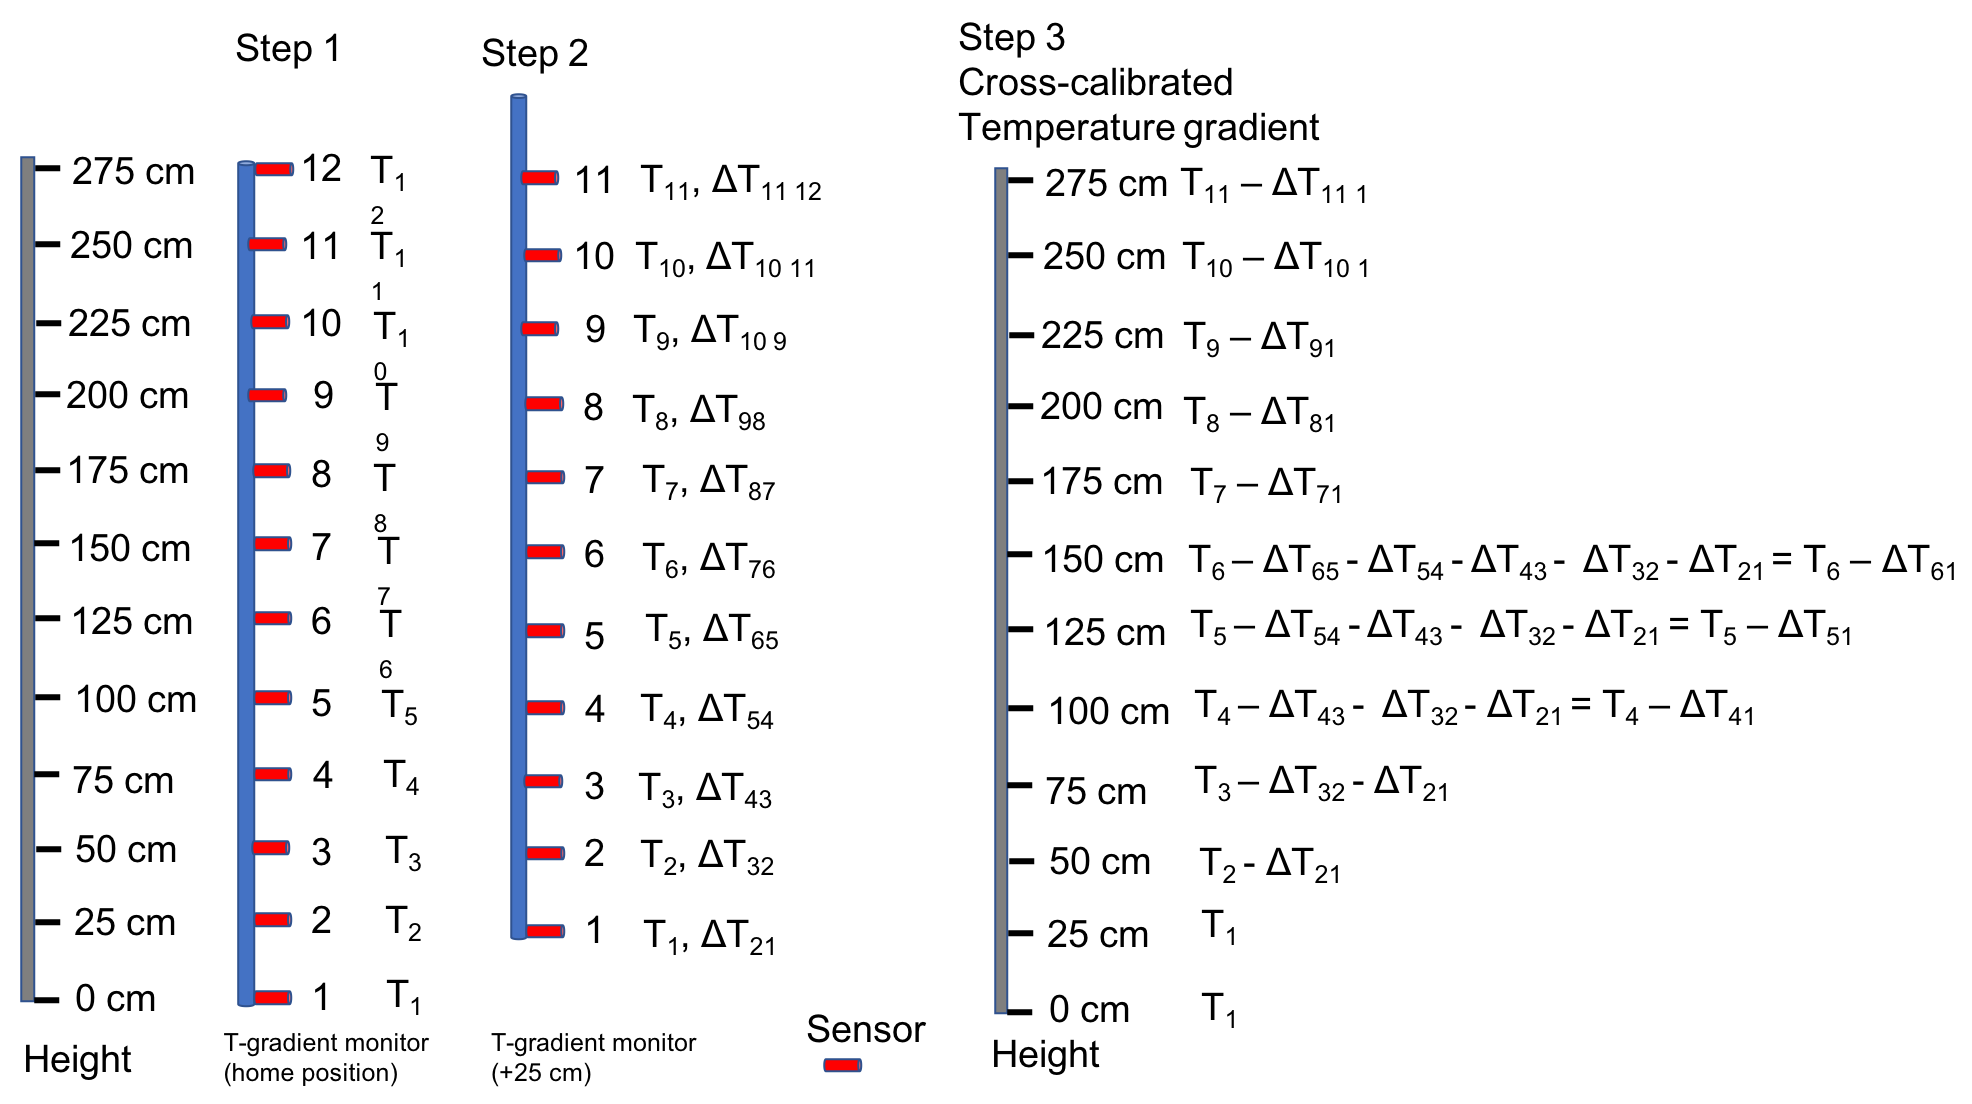
\includegraphics[width=1.0\textwidth]{cisc_cross_calibration_illustration.png}%
\end{dunefigure}


A total of \num{72} sensors will be installed with \SI{25}{cm} spacing, decreased to \SI{10}{cm} spacing for the top and bottom \SI{1}{m} of the carrier rod.  
 The vertical displacement of the system is such that every sensor can be moved to the nominal position of at least five other sensors, minimizing the risks associated with sensor failure and allowing for several points of comparison. The total expected motion range of the carrier rod is \SI{1.35}{m}.

%\fixme{This entire procedure is unclear. Shorten the sentences and make the procedure description more precise. A figure might help, along with references to that figure in the text. {\bf  ANSELMO:  I've removed the existing text and added some text above. The concept is clear, I don't think we need to give more details, which could confuse the reader.} {\em I think it is clear now. =Glenn}} 

%The procedure for cross-calibration involves first, taking a temperature reading at the lowest sensor position. Then, the stepper motor moves the carrier rod up by \SI{50}{cm} putting all sensors in the location of their neighbor that is \SI{50}{cm} above them. Then the second reading is taken. In this manner, except for the lowest position we have temperature measurement at each location with two adjacent sensors, and by linking the temperature offsets between the two readings at each location, temperature readings from all sensors are cross-calibrated {\em in situ}, canceling all offsets due to electromagnetic noise or any parasitic resistances that may have prevailed despite the four point connection to the sensors that should cancel most of the offsets. These measurements are taken with very stable current source, which ensures high precision of repeated temperature measurements over time. The motion of the dynamic T-monitor is stepper motor operated, delivering measurements with high spatial resolution. 

This procedure was tested in \dword{pdsp}, where the system was successfully moved up by a maximum of \SI{51}{cm}, allowing cross-calibration of all sensors (22 sensors with \SI{10.2}{cm} spacing at top and bottom and \SI{51}{cm} in the middle). 
Figure~\ref{fig:cisc-cfd-valid} shows the temperature profile after calibration; the smoothness of the profile demonstrates the reliability of the method. An even better figure of merit is %however 
the temperature profile after cross-calibration, when the recirculation pumps are off. Under these conditions the  temperature should be very homogeneous except near the surface. This is indeed what %is observed in 
Figure~\ref{fig:dynamic_t_pumps-off} shows.  

\begin{dunefigure}[Temperature profile for dynamic T-Gradient with pumps-off]{fig:dynamic_t_pumps-off}
  {Temperature profile as measured by the dynamic T-gradient monitor after cross-calibration, when the recirculation pumps are off. Temperature variation is of the order of \SI{3}{mK} except close to the top and the gas phase interface, as expected.}
  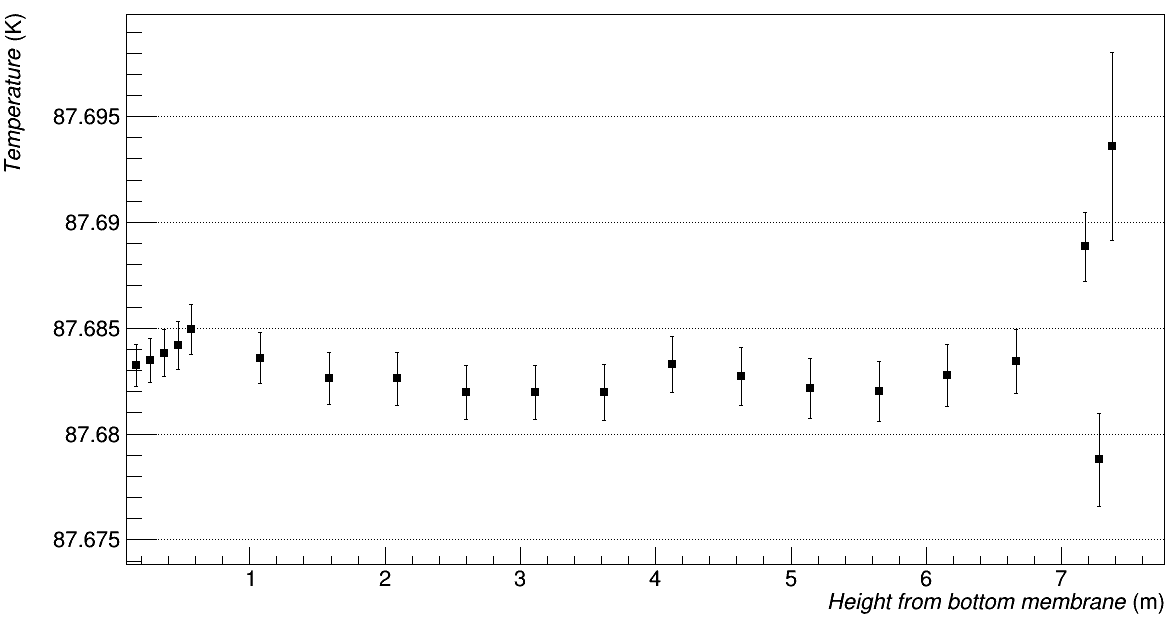
\includegraphics[width=0.6\textwidth]{cisc_dynamic_t_pumps-off.png}%
\end{dunefigure}


%\subsubsection{Dynamic T-gradient monitor design}
%\label{sec:fdgen-slow-cryo-dynamic-therm-design}
A dynamic T-gradient monitor has three parts: a carrier rod on which sensors are mounted; an enclosure above the cryostat housing space that allows the carrier rod to move vertically  \SI{1.5}{m} over its lowest location; and the motion mechanism. The motion mechanism consists of a stepper motor connected through a ferrofluidic dynamic seal to a gear and pinion motion mechanism. The sensors have two pins soldered to a printed circuit board (PCB). 
%\fixme{maybe add gloss term}
Two wires are individually soldered to the common soldering pad for each pin.  A cutout in the PCB around the sensor allows free flow of argon for more accurate temperature readings.  Stepper motors typically have very fine steps that allow highly precise positioning of the sensors.  Figure~\ref{fig:fd-slow-cryo-dt-monitor-overview} shows the overall design of the dynamic T-gradient monitor. % with the sensor carrier rod, enclosure above the cryostat, and stepper motor mounted on the side of the enclosure. 
The enclosure has two parts connected by a six-cross flange. One side of this flange will be used for signal wires, another will be used as a viewing window, and the two other ports will be spares. Figure~\ref{fig:fd-slow-cryo-sensor-mount}, left shows the PCB mounted on the carrier rod and the sensor mounted on the PCB along with the four point connection to the signal readout wires. %Finally, 
Figure~\ref{fig:fd-slow-cryo-sensor-mount}, right shows the stepper motor mounted on the side of the rod enclosure. The motor remains outside the enclosure, at room temperature, %and 
as do its power and control cables. % also remain outside.

\begin{dunefigure}[Dynamic T-gradient monitor overview]{fig:fd-slow-cryo-dt-monitor-overview}
  {%An overview 
  A schematic of the dynamic T-gradient monitor.}
% 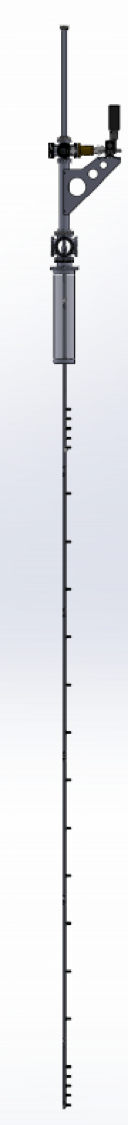
\includegraphics[width=0.11\textwidth,angle=90]{cisc_DTOverview.png}
 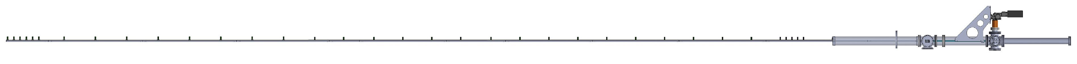
\includegraphics[width=0.95\textwidth,angle=0]{cisc_DynamicProfiler.png}
\end{dunefigure}
\begin{dunefigure}[Sensor-cable assembly for dynamic T-gradient monitor]{fig:fd-slow-cryo-sensor-mount}
  {Left: Sensor mounted on a PCB board and PCB board mounted on the rod. Right:
    The driving mechanism of the dynamic T-gradient monitor, consisting of a stepper motor driving the pinion and gear linear motion mechanism. }
  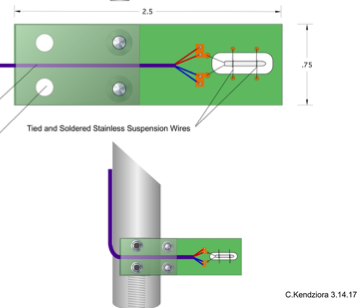
\includegraphics[width=0.40\textwidth]{cisc_DTSensorMount.png}
  \hspace{3cm}%
  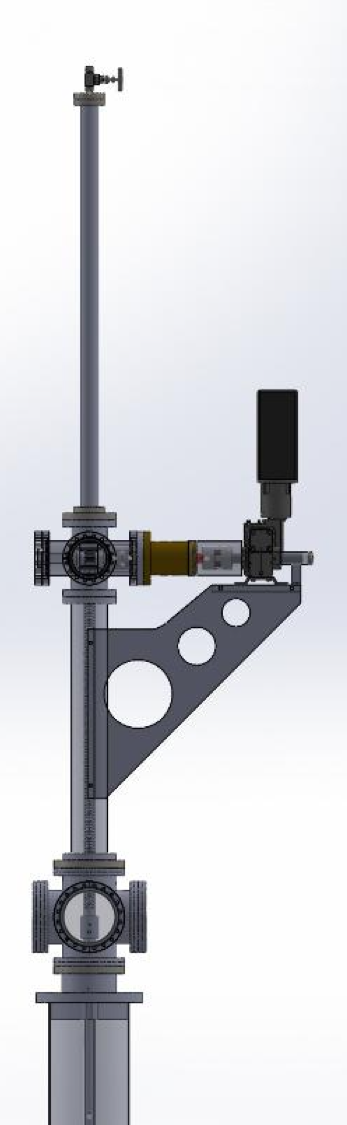
\includegraphics[width=0.12\textwidth]{cisc_DTMotor.png}
\end{dunefigure}

% % % %
\subsubsection{Individual Temperature Sensors}
\label{sec:fdgen-slow-cryo-individual-therm}

T-gradient monitors will be complemented by a coarser 2D array (every \SI{5}{m}) of precision sensors at the top and bottom of the \dword{detmodule}, as shown in Figure~\ref{fig:cisc-tsensor-map}. Following the \dword{pdsp} design, bottom sensors will use the cryogenic pipes as a support structure, while top sensors will be anchored to the \dwords{gp}. Although sensors at the top will have a similar distribution to those at the bottom, %some differences will occur because 
suitable anchoring points at the top and bottom will differ. 

As in \dword{pdsp}, another set of standard sensors will be evenly distributed and epoxied to the bottom membrane. They will detect the presence of \lar when cryostat filling starts. Finally, two vertical arrays of standard sensors will be epoxied to the lateral walls in two opposite vertical corners, with a spacing of \SI{102}{cm} (every three corrugations), to monitor the cryostat membrane temperature during the cooldown and filling processes. 

%While 
Whereas in \dword{pdsp}, cables were routed individually (without touching neighboring cables or any metallic elements) to prevent grounding loops in case the outer Teflon jacket broke, such a failure is very unlikely. Thus, in the \dwords{detmodule}, cables will be routed in bundles, simplifying the design enormously. As Figure~\ref{fig:cisc-tsensor-map} shows, up to 20 sensors will use the same \dword{dss} port, large enough for a cable bundle \SI{16}{mm} in diameter.

Cable bundles of several sizes will be configured using custom made Teflon 
pieces %,  %(see Fig.~\ref{fig:cable-support})
%which 
that will be anchored to different cryostat and detector elements to route cables from sensors to \dword{dss} ports. For sensors at the bottom (on pipes and floor), cables will be routed towards the cryostat bottom horizontal corner using stainless steel split clamps anchored to pipes (successfully prototyped in \dword{pdsp}), and from there, to the top of the cryostat using vertical strings (as with static T-gradient monitors). For sensors on the top \dwords{gp}, cables bundles will be routed to the corresponding \dword{dss} port using Teflon supports attached to both the FR4 threaded rods in the union between two \dword{gp} modules and to the \dword{dss} I-beams (both successfully prototyped in \dword{pdsp}). Sensors on the walls will use bolts in the vertical corners for cable routing. 

For all individual sensors, PCB sensor support, cables, and connection to the flanges will be the same as for the T-gradient monitors. 
  

%\begin{dunefigure}[Cable supports for individual temperature sensors]{fig:cable-support}
%  {Left: support for two cables on ground planes. Right: Supports for three %cables  mounted on cryogenics pipes using split clamps}
% This PDF is made from the .dot of the same name.
%  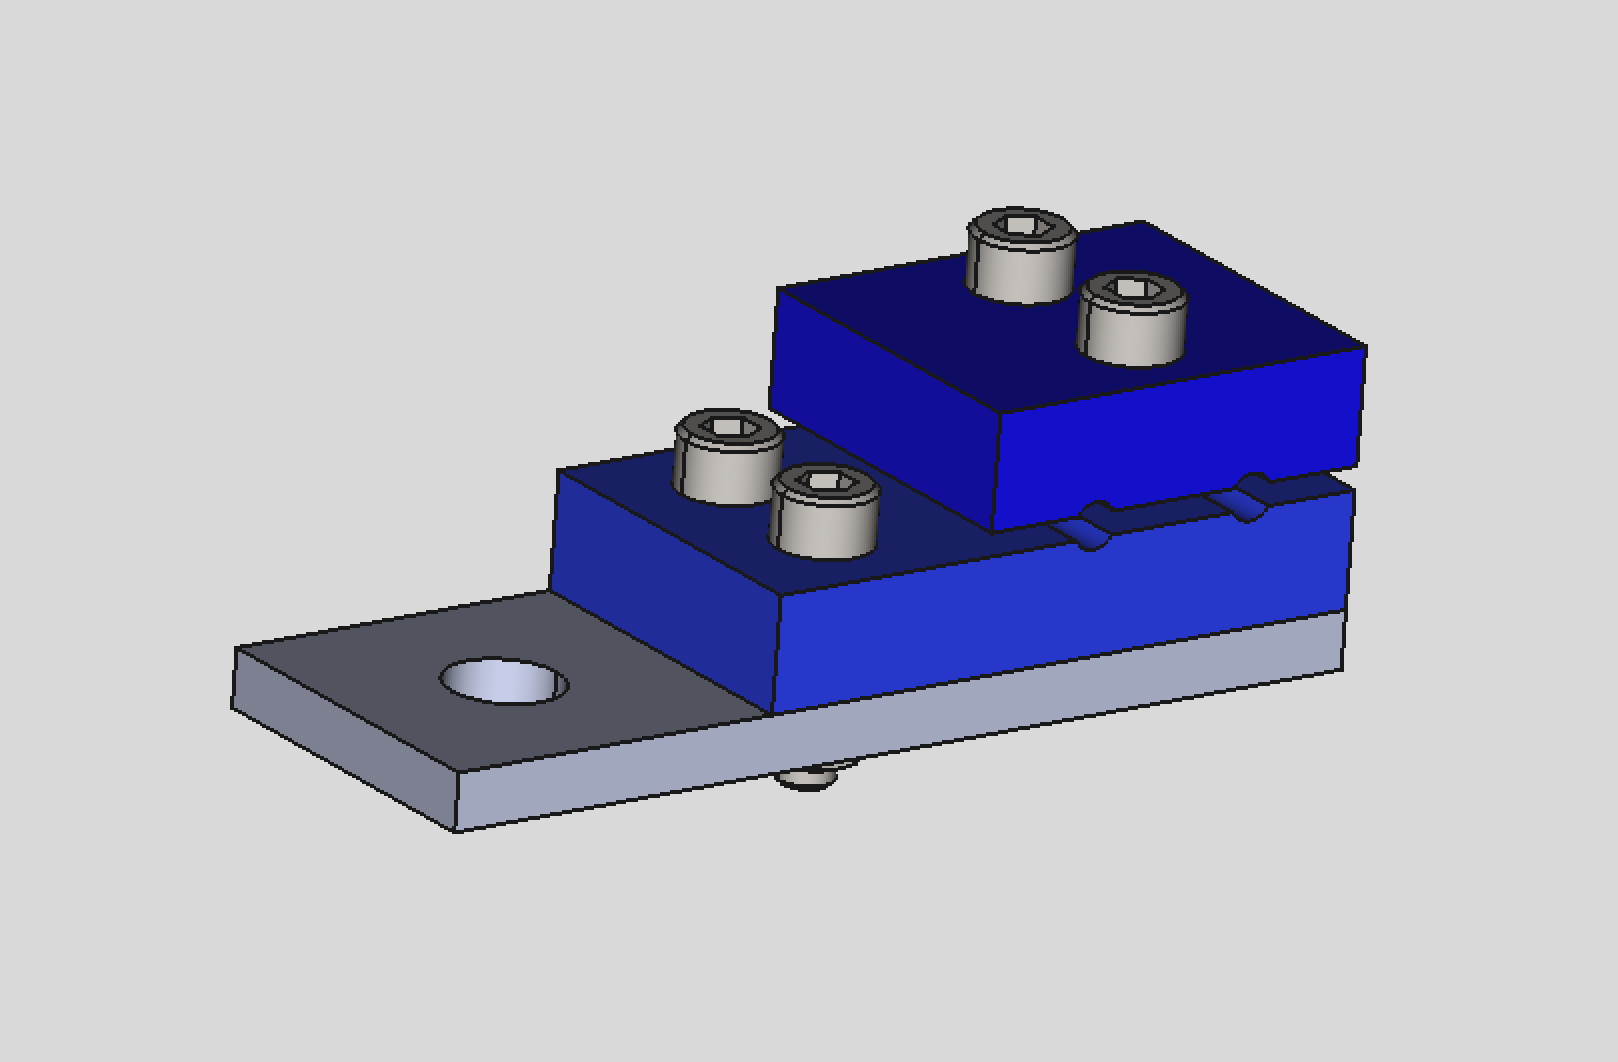
\includegraphics[width=0.3\textwidth]{cisc_TcableSupportGP.png}
%  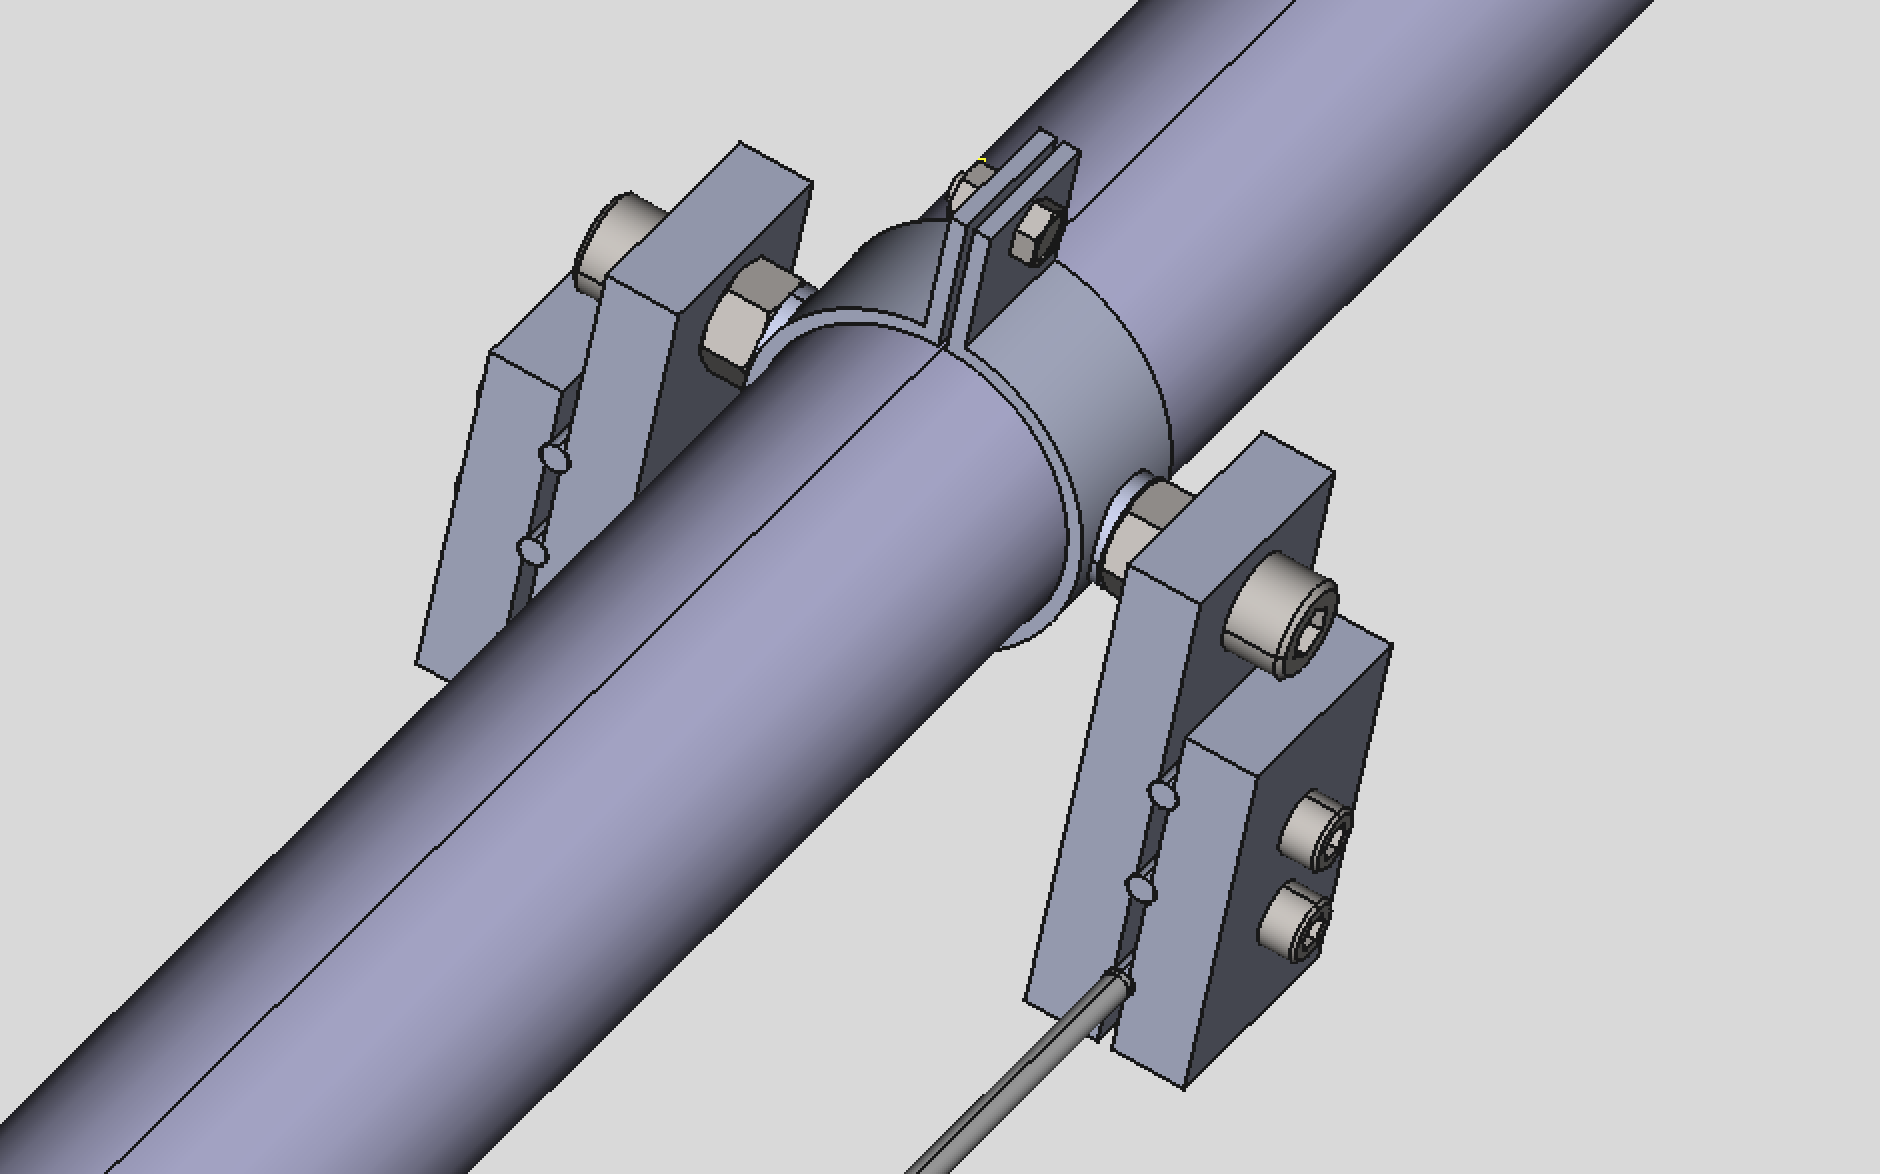
\includegraphics[width=0.315\textwidth]{cisc_TcableSupportPipes.png}
%\end{dunefigure}


% % % %
\subsubsection{Readout system for thermometers}
\label{sec:fdgen-slow-cryo-therm-readout}

A %highly precise 
high-precision and very stable system is required to achieve a readout level of $<\,\SI{5}{mK}$.
The proposed readout system was used in \dword{pdsp} and relies on a variant of an existing mass PT100 temperature readout system developed at
CERN for an LHC experiment; it has already been tested and validated in \dword{pdsp}.
%; it has already been tested and validated by the collaboration experts. 
The system has an electronic circuit that includes
\begin{itemize}
\item a precise and accurate current source for the excitation of the temperature sensors measured using the four-wires method,
\item a multiplexing circuit connecting the temperature sensor signals and forwarding the selected signal to a single line, and 
\item a readout system  with a high-accuracy voltage signal readout module\footnote{National Instrument CompactRIO\texttrademark{} device  with a signal readout NI9238\texttrademark{} module} with 24 bit resolution over a \SI{1}{V} range.
\end{itemize}
This readout system also drives the multiplexing circuit and calculates temperature values. The CompactRIO device is connected to the detector Ethernet network, sending temperature values to the DCS software through a standard OPC UA driver.
%\fixme{These acronyms are not defined- RIO, DCS, OPC, UA. GLENN AND CARMEN TO CHECK}

The current mode of operation averages more than \num{2000} samples taken every second for each sensor. 
Figure~\ref{fig:Trepro} shows the system has a resolution higher than 
\SI{1}{mK}, the RMS of one of the offsets in the stable region.


%%%%%%%%%%%%%%%%%%%% LIQUID LEVEL MONITORING %%%%%%%%%%%%%%%%%%%%
\subsection{Liquid Level Monitoring}
% john L, anselmo
% SP

The goals for the \lar level monitoring system are basic level sensing when filling, and precise level sensing during static operations. 

Filling the cryostat with \lar will take several months. During this operation several systems will be use to monitor the \lar level. 
The first 5.5 m will be covered by cameras and by the vertical arrays of \dwords{rtd} at known heights, since temperature will change drastically 
when the cold liquid reaches each \dword{rtd}. Once the liquid reaches the level of the cryogenic pipes going out of the cryostat, 
the differential pressure between that point and the bottom of the cryostat
can be converted to depth using
the known density of \lar.   Fine tuning of the final \lar level will be done using several capacitive level meters at the top of the cryostat. 

During operation, liquid level monitoring has two purposes:
the \dword{lbnf} cryogenics system uses monitoring to tune the \lar flow, and 
DUNE uses monitoring to guarantee that the top \dwords{gp} are always
submerged %(otherwise, the risk of dielectric breakdown is high). The plan is to keep the \lar surface at least \SI{20}{cm} above
%the \dwords{gp}. 
at least \SI{20}{cm} below the \lar surface to mitigate the risk of dielectric breakdown. This was the value used for the \dword{hv} interlock in \dword{pdsp}. 

The \lar flow 
is tuned using two differential pressure level meters, installed as part of the cryogenics system, one on each side of the \dword{detmodule}.  They 
have a precision of \SI{0.1}{\%}, which corresponds to \SI{14}{mm} at the
nominal \lar surface. Cryogenic pressure sensors will be purchased from commercial sources. Installation methods and positions will be determined as part of the
cryogenics internal piping plan.  
%Sufficient redundancy will be designed in
%to ensure that no single point of failure compromises the level measurement.

%This precision is sufficient for the  \dword{spmod}, since the plan is to keep the \lar surface at least \SI{20}{cm} above the \dwords{gp} (this is the value used for the \dword{hv}
%interlock in \dword{pdsp}); thus, no additional level meters are required for the \single. 

For \dword{hv} integrity, multiple 4~m long capacitive level sensors (with a precision of less than 5~mm) will be deployed along the top of the fluid %, used 
for use during stable operations, and checked against each other.
One capacitive level sensor at each of the four corners of the cryostat will provide sufficient redundancy to ensure that no single point of failure compromises the %capacitive level sensor 
measurement.

% However, in the \dual \lar system the surface level should be controlled at the millimeter level, which can be accomplished with capacitive monitors. Using the same capacitive monitor system in each \dword{detmodule} reduces design differences and provides a redundant system for the \single.  Either system could be used for the \dword{hv} interlock.





Figure~\ref{fig:cisc_pdsp_level} shows the evolution of the \dword{pdsp} LAr level over two months as measured by the differential pressure and capacitive level meters. 
%\fixme{Liquid Level Monitoring has \dword{protodune} results --> \textbf{Anselmo to get data, add something about this. WORK IN PROGRESS}}


\begin{dunefigure}[\lar level measurements]{fig:cisc_pdsp_level}{Evolution of the \dword{pdsp} \lar level over two months. Left: Measured by the capacitive level meter. Right: Measured by the differential pressure level meter. The units in the vertical axis are percentages of the cryostat height (\SI{7878}{mm}).}
  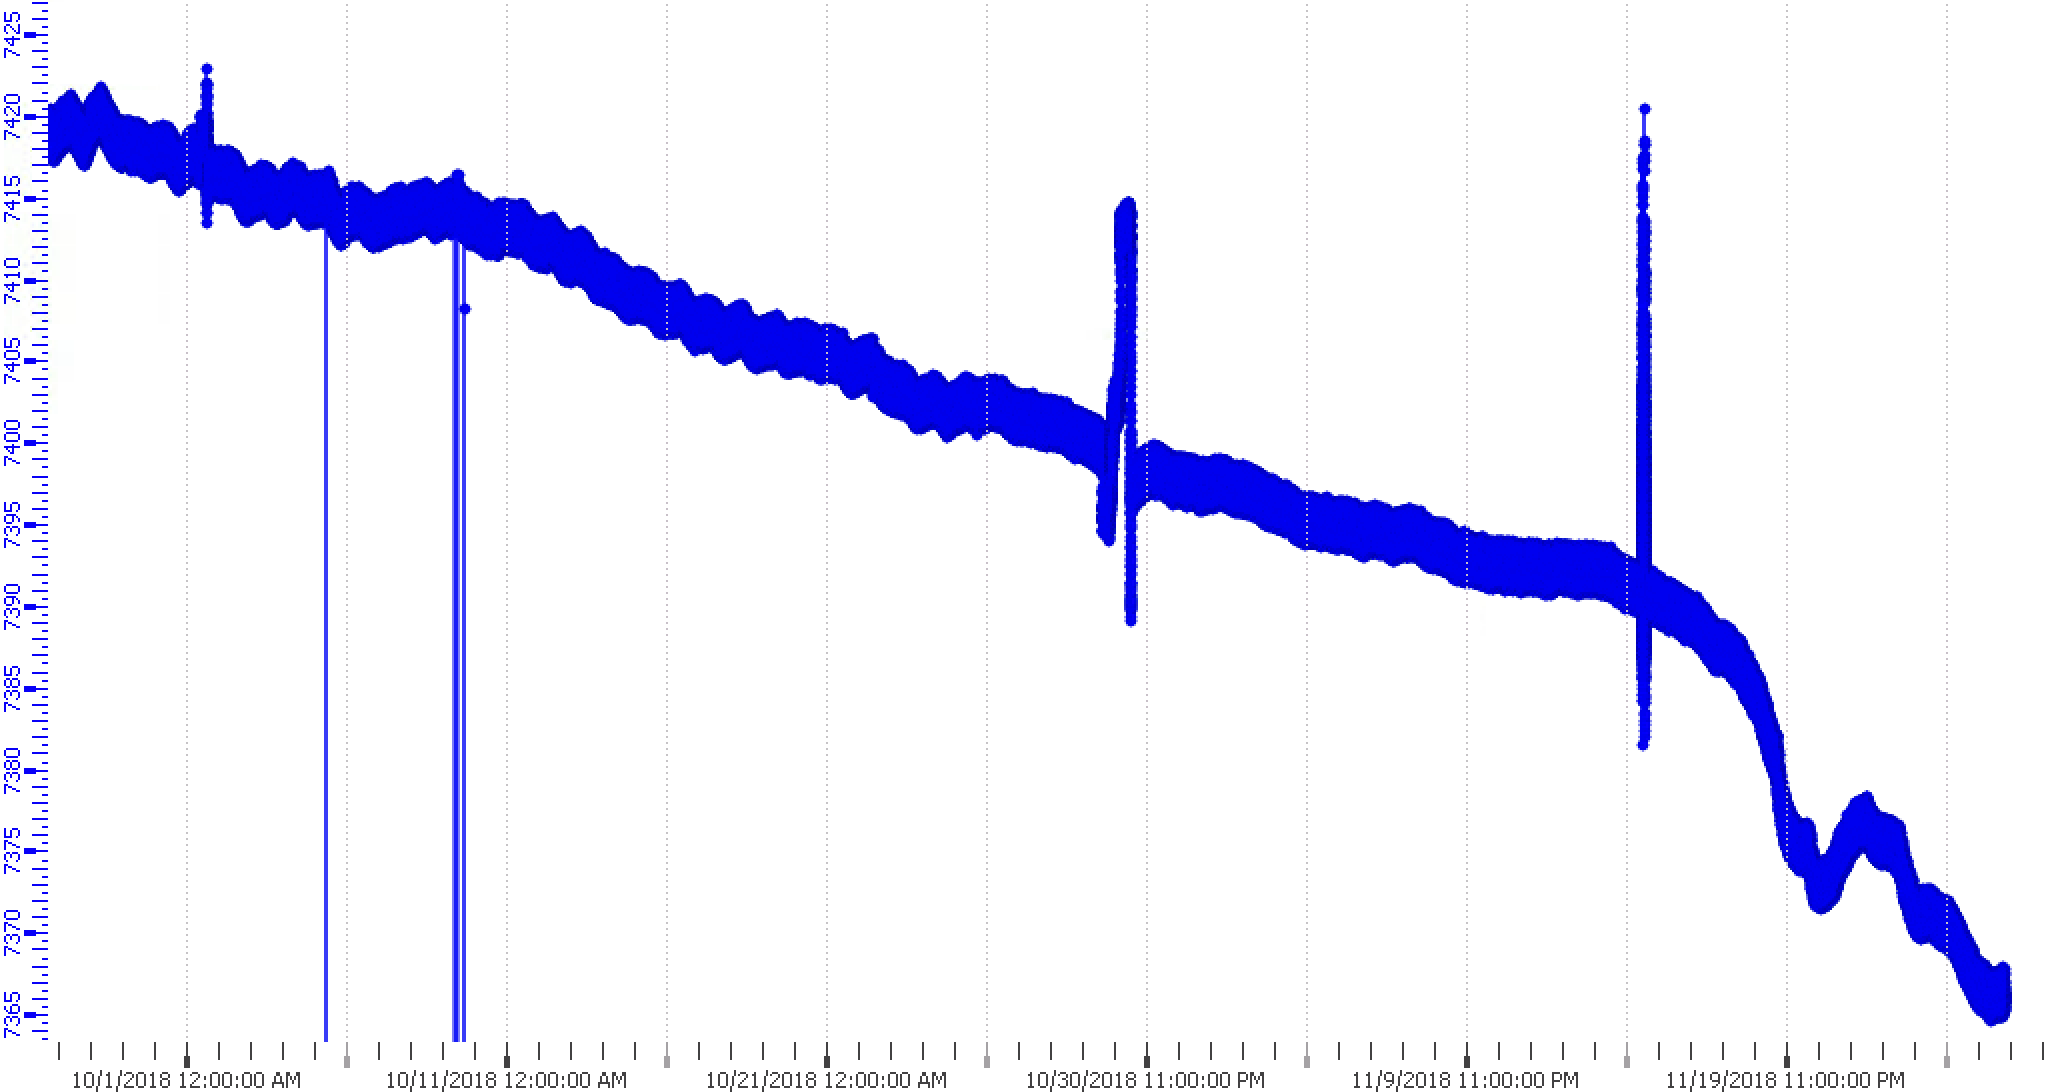
\includegraphics[width=0.4\textwidth]{cisc_level_cap.png}%
  \hspace*{1cm}
  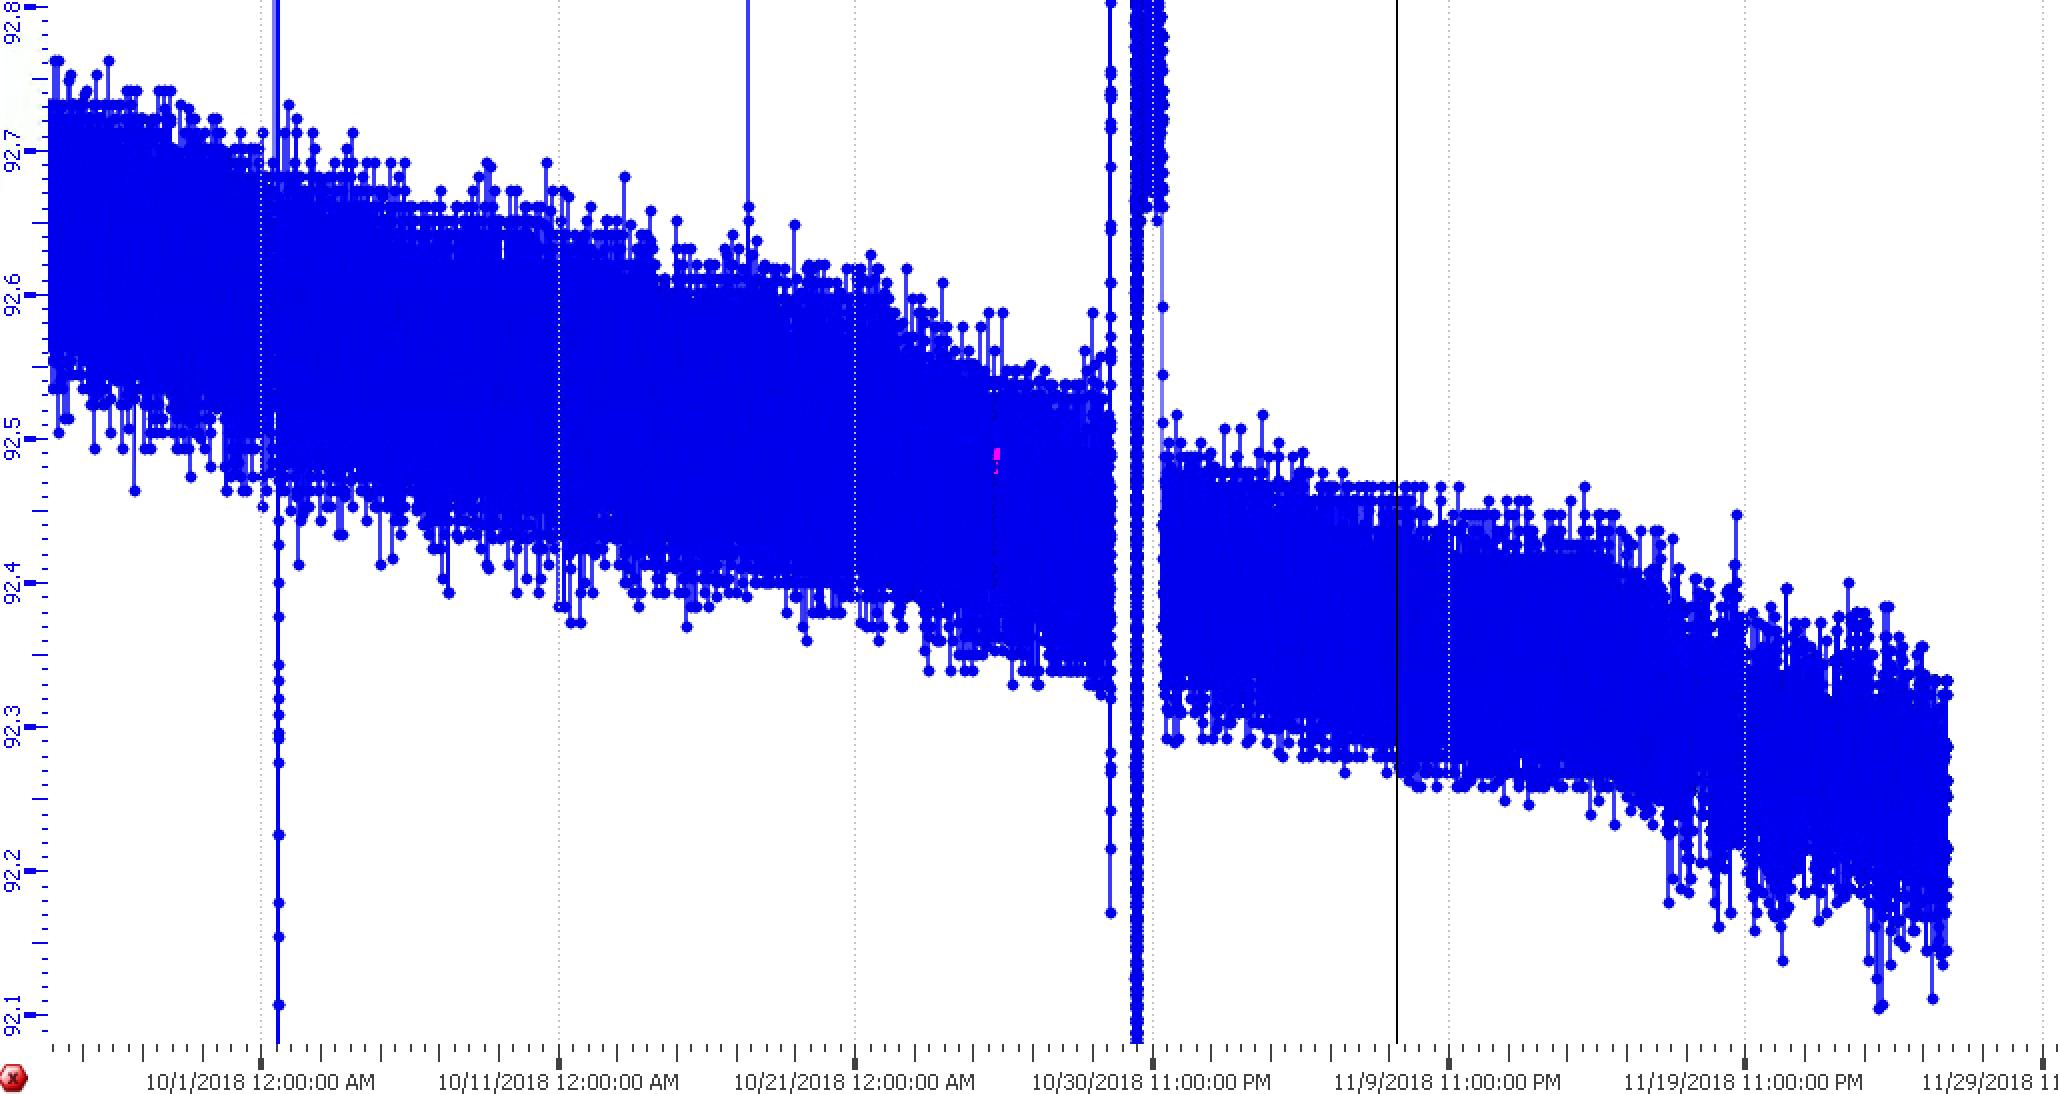
\includegraphics[width=0.4\textwidth]{cisc_level_diffp.png}%
\end{dunefigure}

\dword{pdsp} is using the same design for differential pressure level meters which will also be used in the far detector \dword{spmod}. In the case of capacitive level meters, \dword{pdsp} is using commercially bought 1.5~m long level meters while \dword{pddp} is using 4~m long level meters that are custom-built by CERN. For the DUNE \dword{fd}, we plan to use the longer capacitive level meters custom-built by CERN for both \dword{sp} and \dword{dp} modules.

\subsection{Pressure Meters}
\label{sec:fdgen-slow-cryo-press-meter}

The absolute temperature in the liquid varies with the pressure in the argon gas, therefore, precise measurements of pressure inside the cryostat allows for a better understanding of temperature gradients and \dword{cfd} simulations. In ProtoDUNE, pressure values were also be used to understand the strain gauge signals installed in the cryostat frame.

Standard industrial pressure sensors can be used to measure the pressure of the argon gas in the ullage in the cryostat. For the DUNE \dword{fd}, the plan is to follow the same design and configuration used in \dword{pdsp}. ProtoDUNE uses two types of pressure sensors and a pressure switch as described below:
\begin{itemize}
    \item A relative pressure sensor (range: 0-400~mbar, precision: 0.01~mbar),
    \item An absolute pressure sensor (range: 0-1600~mbar, precision: 0.05~mbar),
    \item A mechanical relative pressure switch adjustable from 50 to 250~mbar. 
\end{itemize}

\begin{dunefigure}[Photo of the pressure sensors installed on a flange in \dword{pdsp}]{fig:pdsp-pressure}
  {Photograph of the pressure sensors installed on a flange in \dword{pdsp}.}
  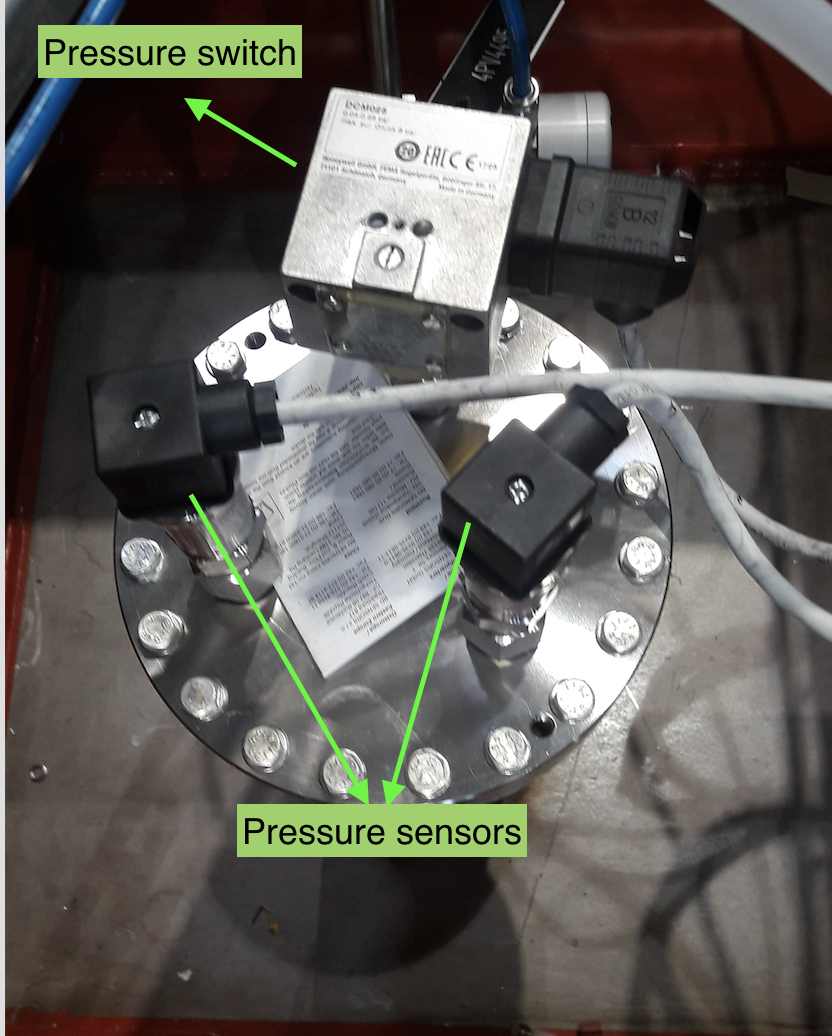
\includegraphics[width=0.5\textwidth]{graphics/cisc-pdsp-pressure-meters.png}
\end{dunefigure}

Both sensors and the pressure switch are installed in a dedicated flange as shown in figure~\ref{fig:pdsp-pressure} and are connected directly to a slow controls system programmable logic control (PLC) circuit. Dedicated analogue inputs are used to read the current values (4 to 20~mA) which are then converted to pressure according to the sensors range. Given the much larger size of DUNE \dword{fd}, the system described above will be doubled for redundancy: two flanges in opposite cryostat sides will be instrumented with three sensors each. 

There are also relative and absolute pressure sensors (with comparatively lower precision) installed by \dword{lbnf} which are also recorded by the slow controls system. %The measurements from high precision sensors will be cross checked with LBNF pressure sensors. 
The availability of two types of sensors from LBNF and CISC allows for redundancy, independent measurements, and cross checks.

%%%%%%%%%%%%%%%%%%% GAS ANALYZERS %%%%%%%%%%%%%%%%%%%%
\subsection{Gas Analyzers}
\label{sec:fdgen-slow-cryo-gas-anlyz}
% alan h

 Gas analyzers are commercially produced modules that measure trace quantities of specific gases contained within a stream of carrier gas. The carrier gas for \dword{dune} is argon, and the trace gases of interest are oxygen ($\text{O}_2$), water ($\text{H}_2\text{O}$), and nitrogen ($\text{N}_2$). $\text{O}_2$ and $\text{H}_2\text{O}$ affect the electron lifetime in \dword{lar} and must be kept below \SI{0.1}{ppb} ($\text{O}_2$ equivalent) while $\text{N}_2$ affects the efficiency of scintillation light production at levels higher than \SI{1}{ppm}.
The argon is sampled from either the argon vapor in the ullage or from the \dword{lar} by using small diameter tubing run from the sampling point to the gas analyzer. Typically, the tubing from the sampling points are connected to a switchyard valve assembly used to route the sample points to the desired gas analyzers (see Figure~\ref{fig:GA-switchyard}).


\begin{dunefigure}[Photo of a gas analyzer switchyard valve assembly]{fig:GA-switchyard}
  {A gas analyzer switchyard that routes sample points to the different gas analyzers.}
  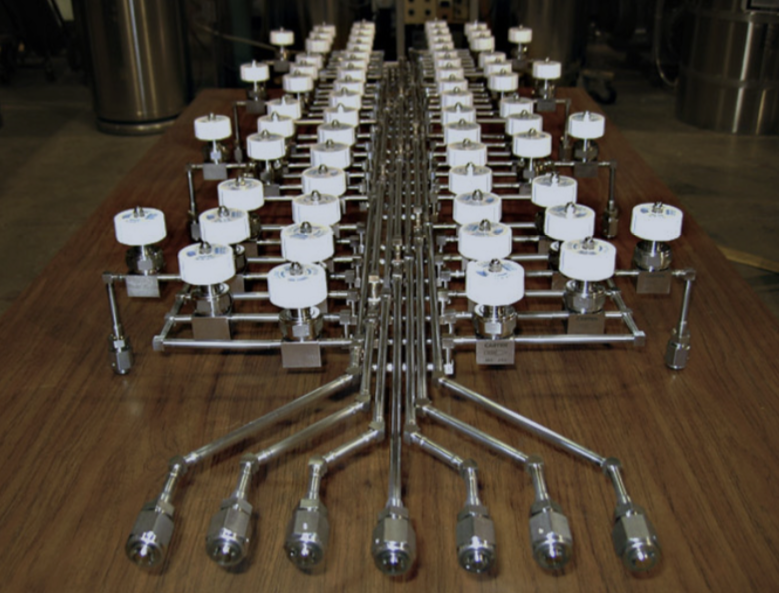
\includegraphics[width=0.9\textwidth]{cisc_GasAnalyzerSwitchyard.png}
\end{dunefigure}

%The following lists three times 
%The gas analyzer would be used three times:
The gas analyzer would be predominantly used during three periods:

\begin{enumerate}
\item Once the detector is installed and after the air atmosphere is eliminated from the cryostat to levels low enough to begin cooldown. This purge and gas recirculation process is detailed in Section~\ref{sec:fdgen-slow-cryo-install-ga}. Figure~\ref{fig:cisc_Phase1_purge_gas_recirculation} shows the evolution of the $\text{N}_2$, $\text{O}_2$, and $\text{H}_2\text{O}$ levels from gas analyzer data taken during the purge and recirculation stages of the \dword{dune} \dword{35t} %Prototype P
phase 1 run.

%\item Track trace $\text{O}_2$ and $\text{H}_2\text{O}$ contaminants from $\>$tens of ppb to hundreds of ppt. This is useful when other means of monitoring impurity levels (e.g., purity monitors, or \dshort{tpc} tracks) are not yet sensitive. Figure~\ref{fig:cisc_O2AnalyzerPrM2_HVRun1} shows an example plot of $\text{O}_2$ levels at the beginning of \dword{lar} purification from one of the later \num{35}\si{t} %Prototype \dword{hv} runs.
\item Before other means of monitoring impurity levels (e.g., purity monitors, or \dshort{tpc} tracks) are sensitive, to track trace $\text{O}_2$ and $\text{H}_2\text{O}$ contaminants from $\>$tens of ppb to hundreds of ppt.  Figure~\ref{fig:cisc_O2AnalyzerPrM2_HVRun1} shows an example plot of $\text{O}_2$ levels at the beginning of \lar purification from one of the later \dword{35t} \dword{hv} runs.

\item During cryostat filling to monitor the tanker \lar delivery purity. This tracks the impurity load on the filtration system and rejects any deliveries that do not meet specifications. %Likely 
Specifications for the delivered \lar are in the \SI{10}{ppm} range per contaminant.

\end{enumerate}

\begin{dunefigure}[Impurity levels during the pre-fill stages for \dword{35t} phase 1]{fig:cisc_Phase1_purge_gas_recirculation}
  {Plot of the $\text{O}_2$, $\text{H}_2\text{O}$, and $\text{N}_2$ levels during the piston purge and gas recirculation stages of the \dword{35t} Phase 1 run}
  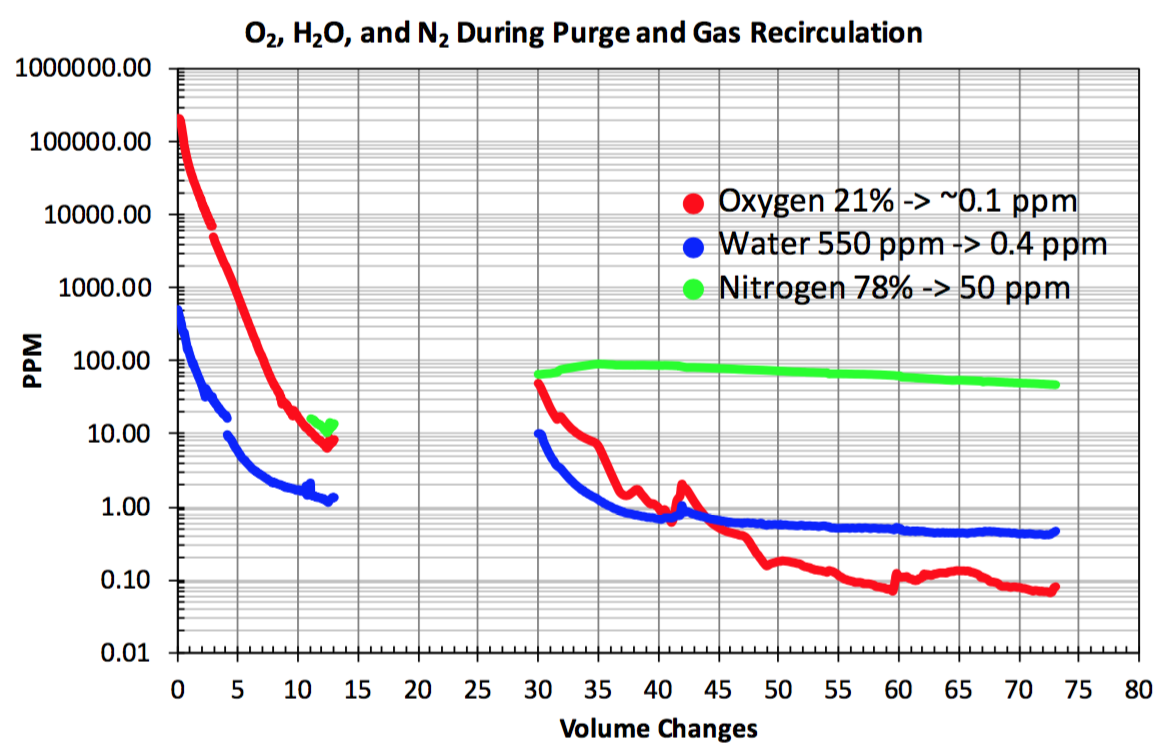
\includegraphics[width=0.7\textwidth]{cisc_Phase1_purge_gas_recirculation.png}
\end{dunefigure}

\begin{dunefigure}[$\text{O}_2$ just after the \dword{35t} was filled with \lar]{fig:cisc_O2AnalyzerPrM2_HVRun1}
  {$\text{O}_2$ as measured by a precision $\text{O}_2$ analyzer just after the \dword{35t} cryostat was filled with \lar, continuing with the \lar pump start and beginning of \lar recirculation through the filtration system. As the gas analyzer loses sensitivity, the purity monitor can pick up the impurity measurement. Note that the purity monitor is sensitive to both $\text{O}_2$ and $\text{H}_2\text{O}$ impurities giving rise to its higher levels of impurity.}
  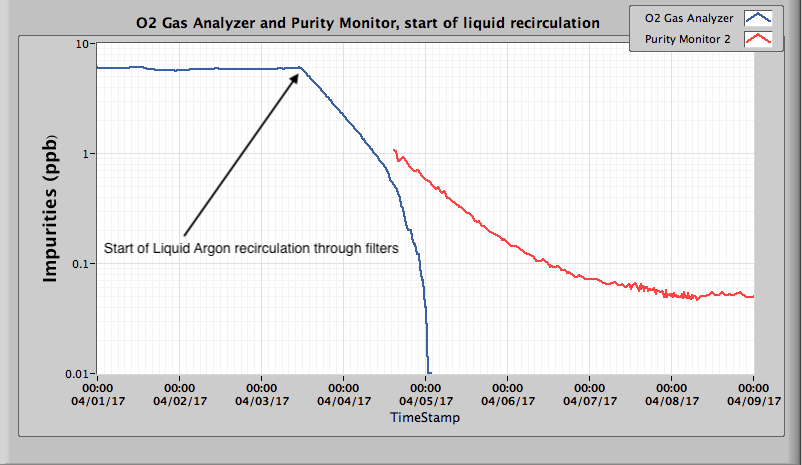
\includegraphics[width=0.7\textwidth]{cisc_O2AnalyzerPrM2_HVRun1.png}
\end{dunefigure}

Because any one gas analyzer covers only one contaminant species and a range of \numrange{3}{4} orders of magnitude, several units are needed both for the three contaminant gases and to cover the ranges seen between  cryostat closure and the beginning of \dshort{tpc} operations:
\SI{20}{\percent} to $\lesssim 100$~ppt for $\text{O}_2$,
\SI{80}{\percent} to $\lesssim 1$~ppm for $\text{N}_2$, and
$\sim \SI{1}{\percent}$ to $\lesssim 1$~ppb for $\text{H}_2\text{O}$.
Because the total cost of these analyzers exceeds $\SI{100}[\mathdollar]{k}$, we want to be able to  sample more than a single location or cryostat with the same gas analyzers. At the same time, the tubing run lengths from the sample point should be as short as possible to maintain a timely response for the gas analyzer. This puts some constraints on sharing devices because, for example, 
a separate gas analyzer may be required in the storage infrastructure for argon delivery at the surface.
%argon is delivered at the surface, so a separate gas analyzer may be required there. %at the surface.

% \fixme{Do Gas Analyzers have \dword{protodune} design and results? Alan and Stephen say they weren't used as extensively at PDSP as at 35t, and "35t is also a prototype and has shown how gas analyzers can be used."}

%%%%%%%%%%%%%%%%%%%%%55 CAMERAS %%%%%%%%%%%%%%%%%%%%%%%%5
\subsection{Cameras}
% glenn, jim s, chuck
% same text in single and dual phase

Cameras provide direct visual information about the state of the
\dword{detmodule} during critical operations and when damage or unusual
conditions are suspected.  Cameras in the \dword{wa105} showed spray from cooldown
nozzles and the level and state of the \lar as it covered the \dword{crp} \cite{Murphy:20170516}.  A camera was
used in the Liquid Argon Purity Demonstrator
cryostat\cite{Adamowski:2014daa} to study \dword{hv} discharges in
\lar and in EXO-100 while a TPC was operating
\cite{Delaquis:2013hva}.  Warm cameras viewing \lar from a distance
have been used to observe \dword{hv} discharges in \lar in
fine detail \cite{Auger:2015xlo}.  Cameras are commonly used during
calibration source deployment in many experiments (e.g., the
\kamland ultra-clean system \cite{Banks:2014hra}).

In \dword{dune}, cameras will verify the stability, straightness,
and alignment of the hanging TPC structures during cooldown and
filling; to ensure that no bubbling occurs near the \dwords{gp}
(\single) or \dwords{crp} (\dual); to inspect the
state of movable parts in the \dword{detmodule} (calibration devices, dynamic
thermometers); and to closely inspect parts of the TPC after any seismic activity or other unanticipated
event.  For these functions, a set of fixed
\textit{cold} cameras are used; they are permanently mounted at fixed points in the cryostat
for use during filling and commissioning, and a movable, replaceable
\textit{warm} inspection camera can be deployed through any free
instrumentation flange at any time during the life of the
experiment. 
% [GAHS: I commented out the table.] Table \ref{tab:fdgen-cameras-req} summarizes the requirements for the camera system.

Eleven cameras were deployed in \dword{pdsp} at the locations shown in Figure~\ref{fig:pdsp-camera-locations}. They successfully provided views of the detector during filling and throughout %the 
its operation. % of the detector.

\begin{dunefigure}[Camera locations in \dword{pdsp}]{fig:pdsp-camera-locations}
  {A \threed view showing the locations of the 11 cameras in \dword{pdsp}.}
  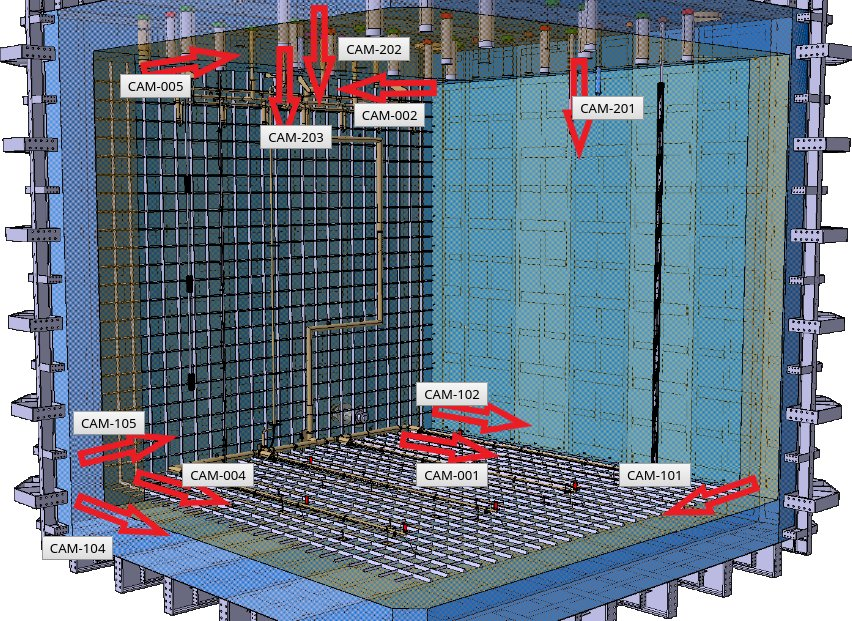
\includegraphics[width=0.6\textwidth]{pdsp-camera-locations-3d}%
\end{dunefigure}

The following sections describe the design considerations for both cold
and warm cameras and the associated lighting system. \dword{pdsp} camera system designs and performance are also discussed.  
The same basic
designs can be used for both the \single and \dual \dwords{detmodule}.

% GAHS: I commented out the table
% \begin{dunetable}
% [Camera system requirements]
% {p{0.45\linewidth}p{0.50\linewidth}}
% {tab:fdgen-cameras-req}
% {Camera system requirements}   
%  Requirement & Physics Requirement Driver \\ \toprowrule
%  \multicolumn{2}{l}{\bf General} \\ \specialrule{1.5pt}{1pt}{1pt}
%  No component may contaminate the \lar{}. & High \lar purity is required for TPC operation. \\ \colhline
%  No component may produce bubbles in the liquid argon if the \dword{hv} is on. & Bubbles increase risk of \dword{hv} discharge. \\ \colhline
%  No point in the camera system shall have a field greater than \SI{15}{kV/cm} when the drift field is at nominal voltage. & Fields must be well below \SI{30}{kV/cm} to avoid risk of \dword{hv} discharge.\\ \colhline
% The camera system shall not produce measurable noise in any detector system. & Low noise is required for TPC operation. \\ \colhline
%  Cameras provide the viewing functionality as agreed upon with the other subsystems for viewing, as documented in the ICDs with the individual systems. \\ \toprowrule
% \multicolumn{2}{l}{\bf Cold cameras}\\ \specialrule{1.5pt}{1pt}{1pt}
% Minimize heat dissipation when camera not in operation. & Do not generate bubbles when \dword{hv} is on. \\ \colhline
% Longevity must exceed \num{18} months. & Cameras must function throughout cryostat filling and detector commissioning. \\ \colhline
% Frame rate \(\geq\SI{10}{\per s}\). & Observe bubbling, waves, detritus, etc. \\ \toprowrule
% \multicolumn{2}{l}{\bf Inspection cameras}\\ \specialrule{1.5pt}{1pt}{1pt}
% Keep heat transfer to \lar low when in operation. & Do not generate bubbles, some use cases may require operation when \dword{hv} is on. \\ \colhline
% Deploy without exposing \lar to air. & Keep \lar free of N2 and other electronegative contaminants. \\ \colhline
% Camera enclosure must be replaceable. & Replace broken camera, or upgrade, throughout life of experiment. \\ \colhline
% {\bf Light emitting system} \\ \colhline
% No emission of wavelengths shorter than \(\SI{400}{nm}\) & Avoid damaging \dword{tpb} waveshifter. Note emitted wavelength shortens significantly with temperature. \\ \colhline
% Longevity must exceed \num{18} months. & Lighting for fixed cameras must function throughout cryostat filling and detector commissioning. \\ \colhline
% \end{dunetable}

%\fixme{Cameras intro: GAHS -- do we want to keep the separate, lower-level table of requirements for cameras?  I think we have to put key high-level requirements in the requirements table in the Requirements section, and drop this table. [dropped, but need to check for things to add to Requirements]}

%%%%%%%%%%%%%%%%%%%%%%%%%%%%%%%%%%%%%%%
\subsubsection{Cryogenic Cameras (Cold)}

The fixed cameras
monitor the following items during filling:
\begin{itemize}
\item positions of corners of \dword{apa} or \dword{crp}, \dword{cpa} or cathode, \dwords{fc}, \dwords{gp} (\SI{1}{mm} resolution)
\item relative straightness and alignment of \dword{apa} or \dword{crp}, \dword{cpa} or cathode, and \dword{fc} (\(<\sim\SI{1}{mm}\))
\item relative positions of profiles and endcaps (\SI{0.5}{mm} resolution); and 
\item the \lar surface, specifically, the presence of bubbling or debris.
\end{itemize}


% GAHS: I commented out the (pre-\dword{protodune}) past performance discussion because the PDSP cameras performed so well.
% There are published articles and unpublished presentations describing
% completely or partially successful operation of low-cost,
% off-the-shelf \dword{cmos} cameras in custom enclosures immersed in cryogens.
% (e.g., EXO-100: \cite{Delaquis:2013hva}; \dword{dune} \dword{35t} test
% \cite{McConkey:2016spe}; \dword{wa105}: \cite{Murphy:20170516}.)  Generally
% it is reported that such cameras show poor performance and ultimately
% fail to function below some temperature of order \SIrange{150}{200}{K}, but some report that their cameras recover fully after
% being stored (not operated) at temperatures as low as \SI{77}{K} and
% then brought up to minimum operating temperature.

% However, as with photon sensors, experience has also shown that it is
% non-trivial to ensure reliable and reproducible mechanical and
% electrical integrity of such cameras in the cryogenic environment 
% (e.g., \cite{McConkey:2016spe} and
% \cite{Valencia-Rodriquez:20180130}).  Off-the-shelf cameras and camera
% components are generally only specified by the vendors and original
% manufacturers for operation down to \SI{-40}{\celsius} or \SI{-50}{\celsius}.
% In addition, many low-cost cameras use digital interfaces not intended
% for long distance deployment, such as USB (\(2\sim\SI{5}{m}\)) or CSI (circuit
% board scale), leading to signal degradation and noise problems.

One design for the \dword{dune} fixed cameras uses an enclosure similar to
the successful EXO-100 design \cite{Delaquis:2013hva}, which was also
successfully used in the Liquid Argon Purity Demonstrator
and \dword{pdsp} (see Figure~\ref{fig:gen-fdgen-cameras-enclosure}). Cameras 101, 102, 104, and 105, shown in Figure~\ref{fig:pdsp-camera-locations}, use this enclosure.
A thermocouple in the enclosure allows temperature monitoring, and a heating element provides temperature control.  
SUB-D connectors are used at the cryostat flanges and the camera enclosure for signal, power, and control connections.
% The enclosure is connected to a stainless steel gas line to allow it to be flushed with argon gas at low enough pressure to prevent liquification, using the same design as the gas line for the beam plug tested in the \dword{35t} \dword{hv} test and in \dword{protodune}.  
%The camera transmits its video signal using either a composite video signal over shielded coax or Ethernet over optical fiber.  Most importantly, the \dword{dune} \dword{cisc} consortium must work with vendors to design camera circuit boards that are robust and reliable in the cryogenic environment.

\begin{dunefigure}[A camera enclosure]{fig:gen-fdgen-cameras-enclosure}
  {Top left: a CAD exploded view of a vacuum-tight camera enclosure suitable for cryogenic applications \cite{Delaquis:2013hva}.
    (1) quartz window, (2 and 7) copper gasket, (3 and 6) flanges, (4) indium wires, (5) body piece, (8) signal \fdth.
    Top right: two of the \dword{pdsp} cameras using a stainless steel enclosure. 
    Bottom left: one of the \dword{pdsp} cameras using acrylic enclosure.
    Bottom right: a portion of an image taken with \dword{pdsp} camera 105 showing a purity monitor mounted outside the \dword{apa} on the beam left side. This photo was taken with \dword{pdsp} completely filled.
  }
  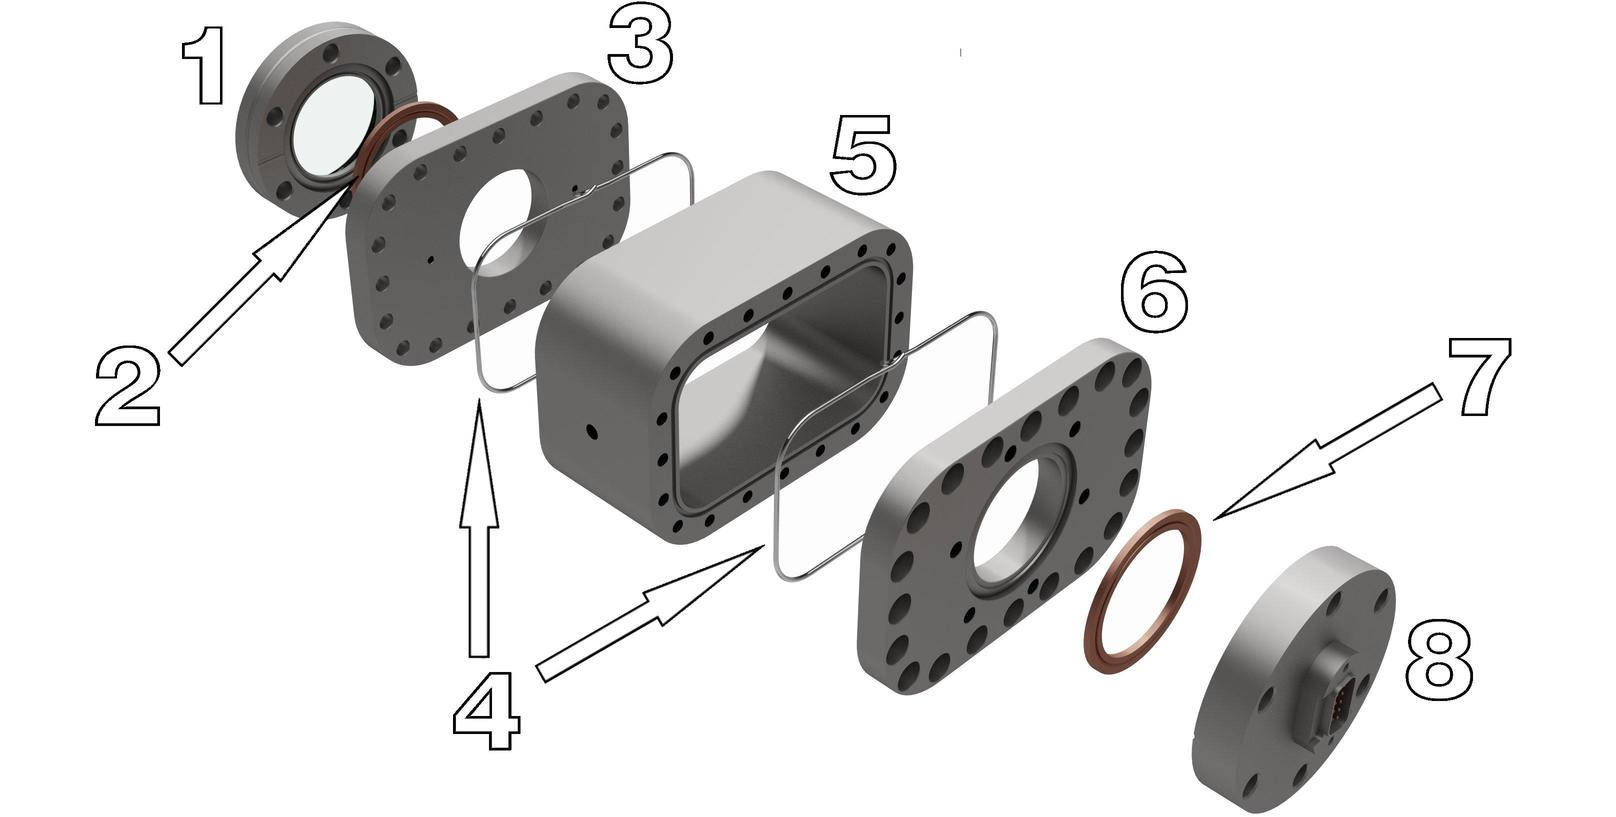
\includegraphics[width=0.4\textwidth]{exo100-camera-case}%
  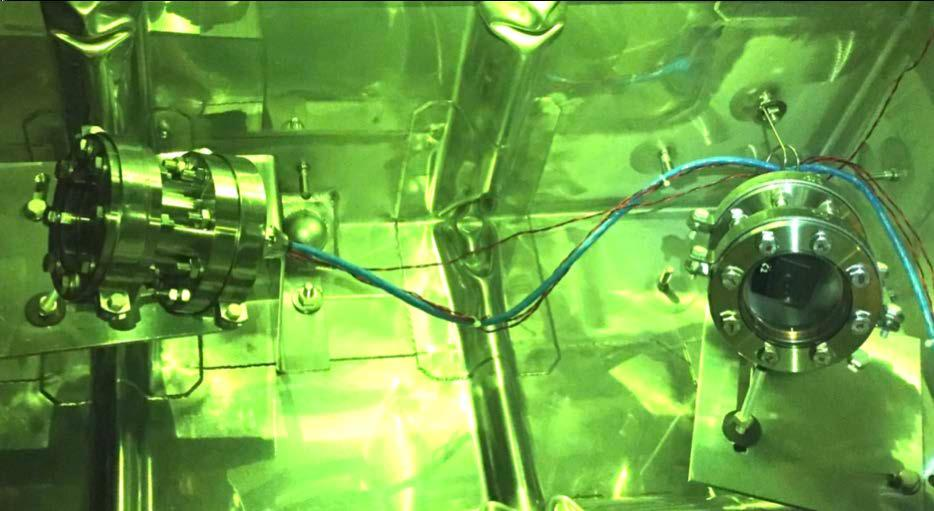
\includegraphics[width=0.4\textwidth]{edgar-cameras}\\
  \hfill 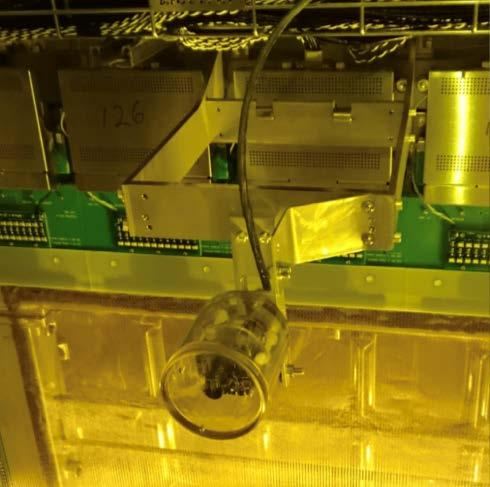
\includegraphics[width=0.22\textwidth]{bo-camera}%
  \hfill 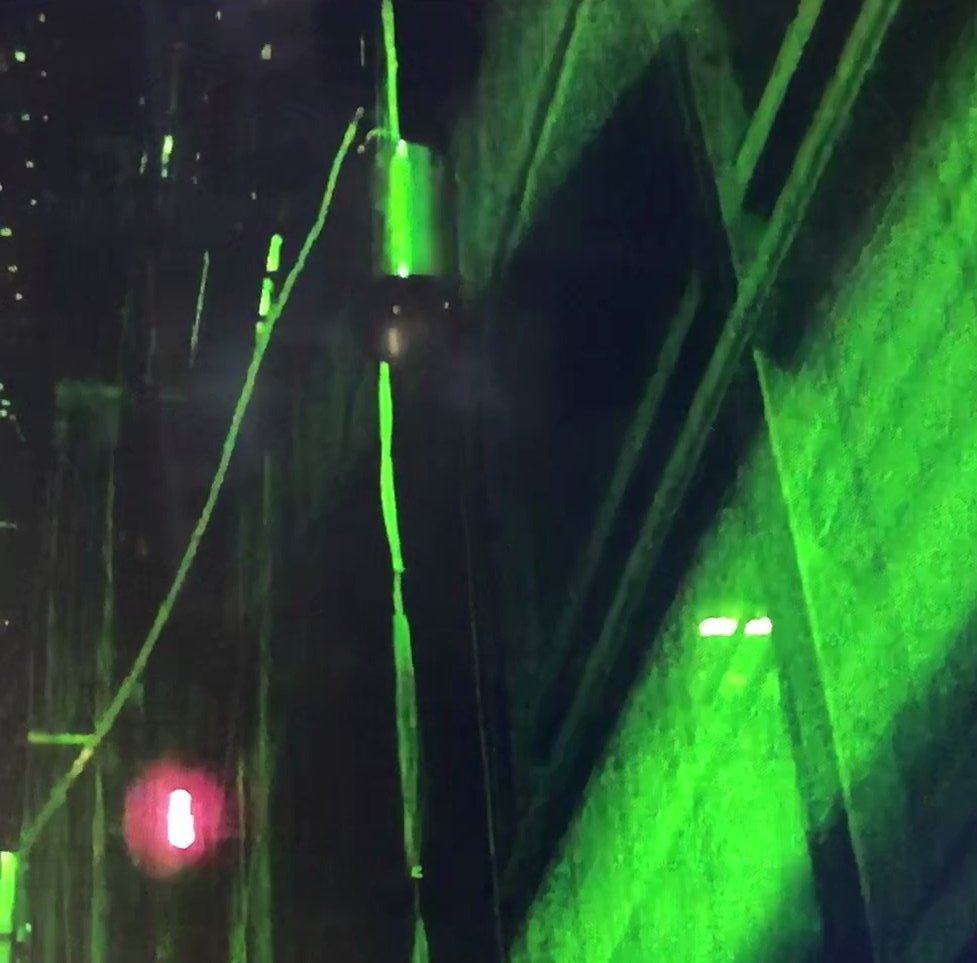
\includegraphics[width=0.22\textwidth]{camera-105-purmon-orig-rot-crop}%
  \hfill
\end{dunefigure}

An alternative design uses an acrylic enclosure.
This design was used successfully in \dword{pdsp} (see Figure~\ref{fig:gen-fdgen-cameras-enclosure}, bottom left). Cameras 001, 002, 004, and 005, shown in Figure~\ref{fig:pdsp-camera-locations}, use acrylic enclosures. 
All operate successfully, including those at the bottom of the cryostat.  It must be noted that the \dword{dune} \dword{fd} will be twice as deep as \dword{protodune}, and therefore cameras observing the lowest surfaces of the \dword{fc} must withstand twice the pressure.

We will continue prototyping and testing in order to finalize and validate the cold camera design for \dword{dune}, focusing particularly on pressure resistance.


%%%%%%%%%%%%%%%%%%%%%%%%%%%%%%%%%%%%%%%%%%%%%%%5
\subsubsection{Inspection Cameras (Warm)}

The inspection cameras are intended to be as versatile as possible.
However, the following %locations 
inspections have been identified as likely uses:
%to be of interest:
\begin{itemize}
\item status of \dword{hv} \fdth and cup,
\item status of \dword{fc} profiles, endcaps (\SI{0.5}{mm} resolution),
\item vertical deployment of calibration sources,
\item status of thermometers, especially dynamic thermometers,
\item \dword{hv} discharge, corona, or streamers on \dword{hv} \fdth, cup, or \dword{fc},
\item relative straightness and alignment of \dword{apa}/\dword{crp}, \dword{cpa}/cathode, and \dword{fc} (\SI{1}{mm} resolution),
\item gaps between \dword{cpa} frames (\SI{1}{mm} resolution),
\item relative position of profiles and endcaps (\SI{0.5}{mm} resolution), and 
\item sense wires at the top of outer wire planes in \single \dword{apa} (\SI{0.5}{mm} resolution).
\end{itemize}

Unlike the fixed cameras, the inspection cameras must operate only as
long as inspection lasts; the cameras can be replaced in case of failure.  It
is also more practical to keep the cameras continuously warmer than
 \SI{-150}{\celsius} during deployment; this allows use of  %and therefore we willhave 
commercial cameras, %more easily, e.g., %.  For example, we could deploy 
e.g., cameras of the same model were used successfully to observe discharges
in \lar from \SI{120}{cm} away \cite{Auger:2015xlo}.


\begin{dunefigure}[Inspection camera design]{fig:gen-fdgen-cameras-movable}
  {Left: An overview of the inspection camera design using a sealed deployment system opening directly into the cryostat. Right: A photo of the \dword{pdsp} warm inspection camera acrylic tube, immediately before installation; the acrylic tube is sealed with an acrylic dome at the bottom and can be opened at the top.}
  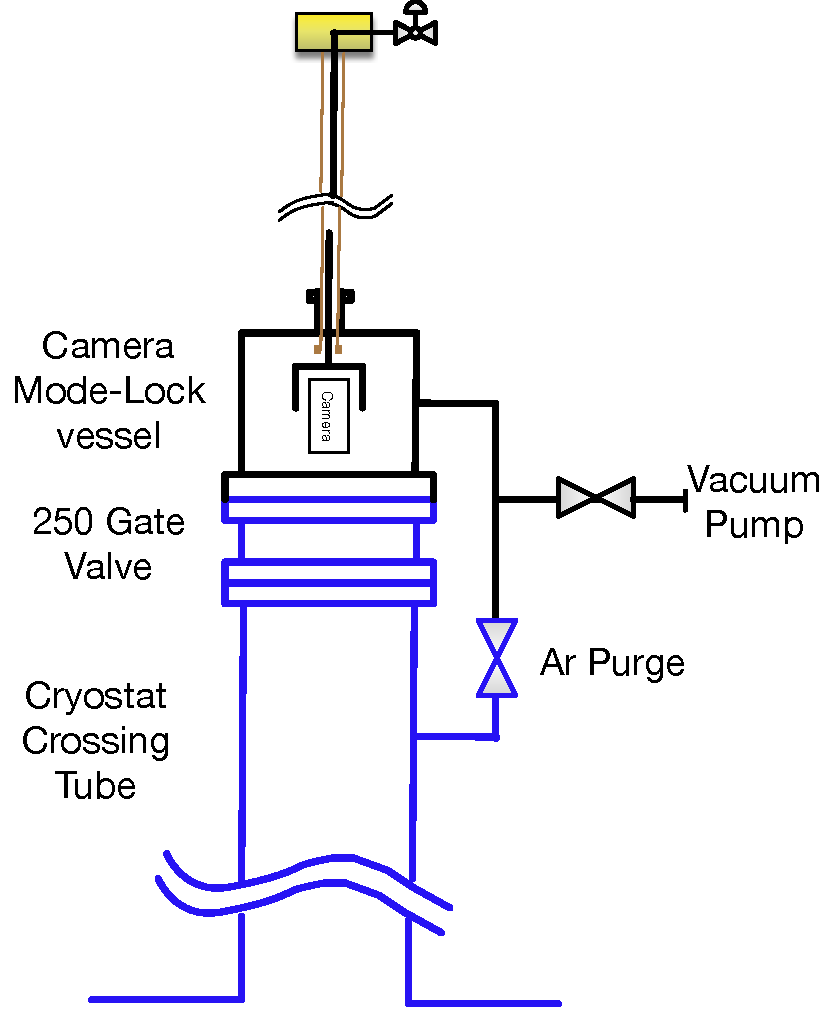
\includegraphics[height=0.3\textheight]{Camera-Sketch}%
  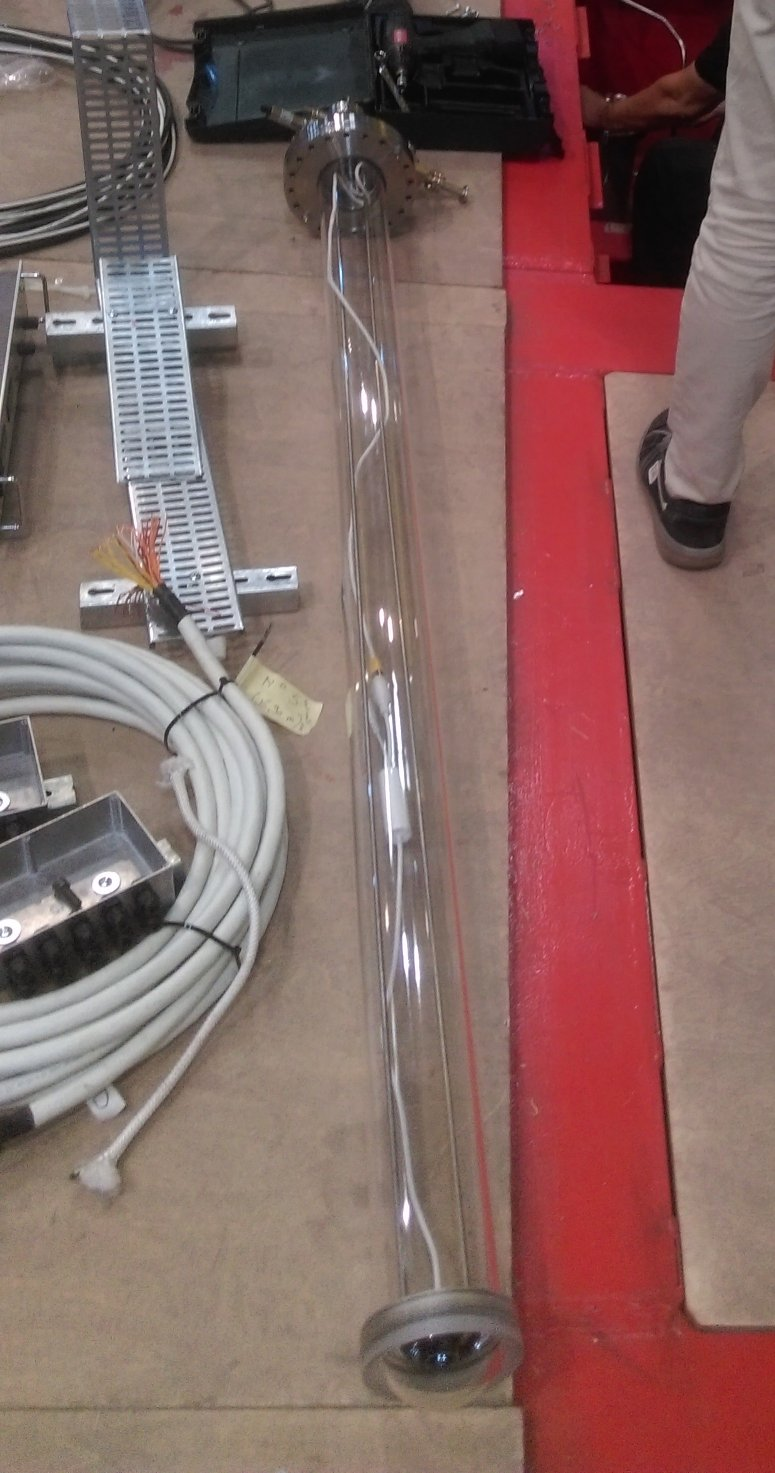
\includegraphics[height=0.3\textheight]{cisc-pdsp-camera-tube}%
\end{dunefigure}

The inspection cameras use the same basic
enclosure design as for cold cameras, but the cameras are mounted on a movable
fork so that each camera can be inserted and removed from the cryostat,
using a design similar to the dynamic temperature probes: see
 Figure~\ref{fig:gen-fdgen-cameras-movable} (left) and
 Figure~\ref{fig:fd-slow-cryo-sensor-mount}.  To avoid contaminating the
\lar with air, the entire system is sealed, and the
camera can only be deployed through a \fdth equipped with a gate
valve and a purging system, similar to the one used in the vertical axis
calibration system at \kamland~\cite{Banks:2014hra}. The entire system
is  purged with pure argon gas before the gate valve is opened.

Motors above the flange allow the fork to be rotated and moved vertically to position the camera. 
 A chain drive system with a motor
mounted on the end of the fork allows the camera assembly to tilt, 
creating a point-tilt mount that can be moved vertically.
With the space above the cryostat flanges and the
thickness of the cryostat insulation, cameras can be moved vertically up to
\SI{1}{m} inside the cryostat.
% In the event that it
% becomes necessary to deploy a camera more deeply, we would have the
% option of building a cable deployment system or a multi-pole
% deployment system similar to the KamLAND full-volume calibration
% system\cite{Busenitz:2009ac}, but this is not currently part of the
% baseline design.
The motors for rotation and vertical motion are outside the sealed
volume, coupled mechanically using ferrofluidic seals, thus reducing any risk of
contamination and allowing manual rotation of the vertical
drive in the event of motor failure.  

An alternative design was demonstrated in \dword{pdsp}. In this design, the warm camera is contained inside a gas-tight acrylic tube inserted into the feedthrough, so a gate valve or a gas-tight rotatable stage is not needed, and the warm cameras can be removed for servicing or upgrade at any time. Figure~\ref{fig:gen-fdgen-cameras-movable} (right) shows an acrylic tube enclosure and camera immediately before deployment. These acrylic tube enclosures for removable cameras were deployed at the positions marked 201, 202, and 203 in Figure~\ref{fig:pdsp-camera-locations}; they operated successfully in \dword{pdsp}. Cameras with fisheye lenses were used in these tubes during initial operation.  One camera was removed without any evidence of contamination of the \dword{lar}. We plan to use other cameras during post-beam running.

We will continue prototyping and testing in order to finalize and validate the inspection camera design for \dword{dune}, focusing particularly on longevity, camera replaceability, and protection of the \dword{lar}.


%%%%%%%%%%%%%%%%%%%%%%%%%%%%%%%%%%%%%%%
\subsubsection{Light-emitting system}
%%% same text as dual-phase
The light-emitting system uses \dwords{led} to illuminate
the parts of the %\dword{fd} 
\dword{detmodule} in the camera's field of view with selected
wavelengths (IR and visible) that cameras can detect.  Performance criteria for the light-emission system include the efficiency with which the cameras can detect the light and the need to avoid
adding heat to the cryostat. Very high-efficiency
\dwords{led}   
help reduce heat generation; one \SI{750}{nm} \dword{led} \cite{lumileds-DS144-pdf}
has a specification equivalent to
\SI{33}{\%} conversion of electrical input power to light.
% CEL: 1W electrical gives 425mW blue flux, power limit from SMD package thermal resistance of 8C/W to have max 1C increase at LED. CREE Xlamp XP-E model

While data on how well \dwords{led} perform at cryogenic temperatures
is sparse, some studies of NASA projects~\cite{Carron:2017zzz}
indicate that \dword{led} are more efficient at low temperatures and
that emitted wavelengths may change, particularly for blue
\dwords{led}.  Amber \dwords{led} were observed in \dword{pdsp} to
emit green light at \dword{lar} temperature. (See bottom right photo
in \ref{fig:gen-fdgen-cameras-enclosure}.)  To avoid degradation of
wavelength-shifting materials in the \dword{pds}, short wavelength
\dwords{led} are not used in the \dword{fd}.

\begin{dunefigure}[Example schematic for LED chain]{fig:cisc-LED}
  {Example schematic for LED chain, allowing failure tolerance and two LED illumination spectra.}
  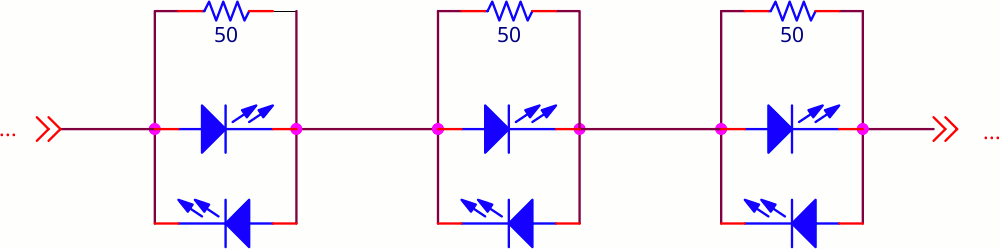
\includegraphics[width=0.6\textwidth]{cisc_led.png}
\end{dunefigure}

\dwords{led} are placed in a ring around the outside of each
camera, pointing in the same direction as the lens, to 
illuminate nearby parts of the \dword{detmodule} within the camera's field of
view. Commercially available \dwords{led} exist with
a range of angular spreads that can be matched to the needs of the
cameras without additional optics.

Additionally, chains of \dwords{led} connected in series and driven with a
constant-current circuit are used for broad illumination, with each
\dword{led} paired in parallel with an opposite polarity \dword{led} and a resistor
(see Figure~\ref{fig:cisc-LED}).
This allows two different wavelengths of illumination using a single chain simply by changing the direction of the drive current, and allows continued use of an \dword{led} chain even if individual \dwords{led} fail.



%%%%%%%%%%%%%%%%%% CRYOGENIC Instrumentation TEST FACILITY %%%%%%%%%%%%%%%%%%%%
\subsection{Cryogenic Instrumentation Test Facility}
% same for SP and DP
% alan h

The \dfirst{citf} at \fnal has provided access to small ($<\,\SI{1}{ton}$) to intermediate ($\sim\,\SI{1}{ton}$) volumes of purified TPC-grade \dword{lar}, required for %. Hardware that requires this high-purity liquid includes 
any device intended for drifting electrons for millisecond periods. %Not all devices need this high purity \lar , but may need a relatively large volume for the necessary prototyping environments. A relatively fast turn-around time of approximately a week is needed for short prototyping runs. 

%\begin{dunefigure}[]{fig:cisc_PAB_photo}
%  {Photo of PAB Cryogenic Test Facility at \fnal.}
%  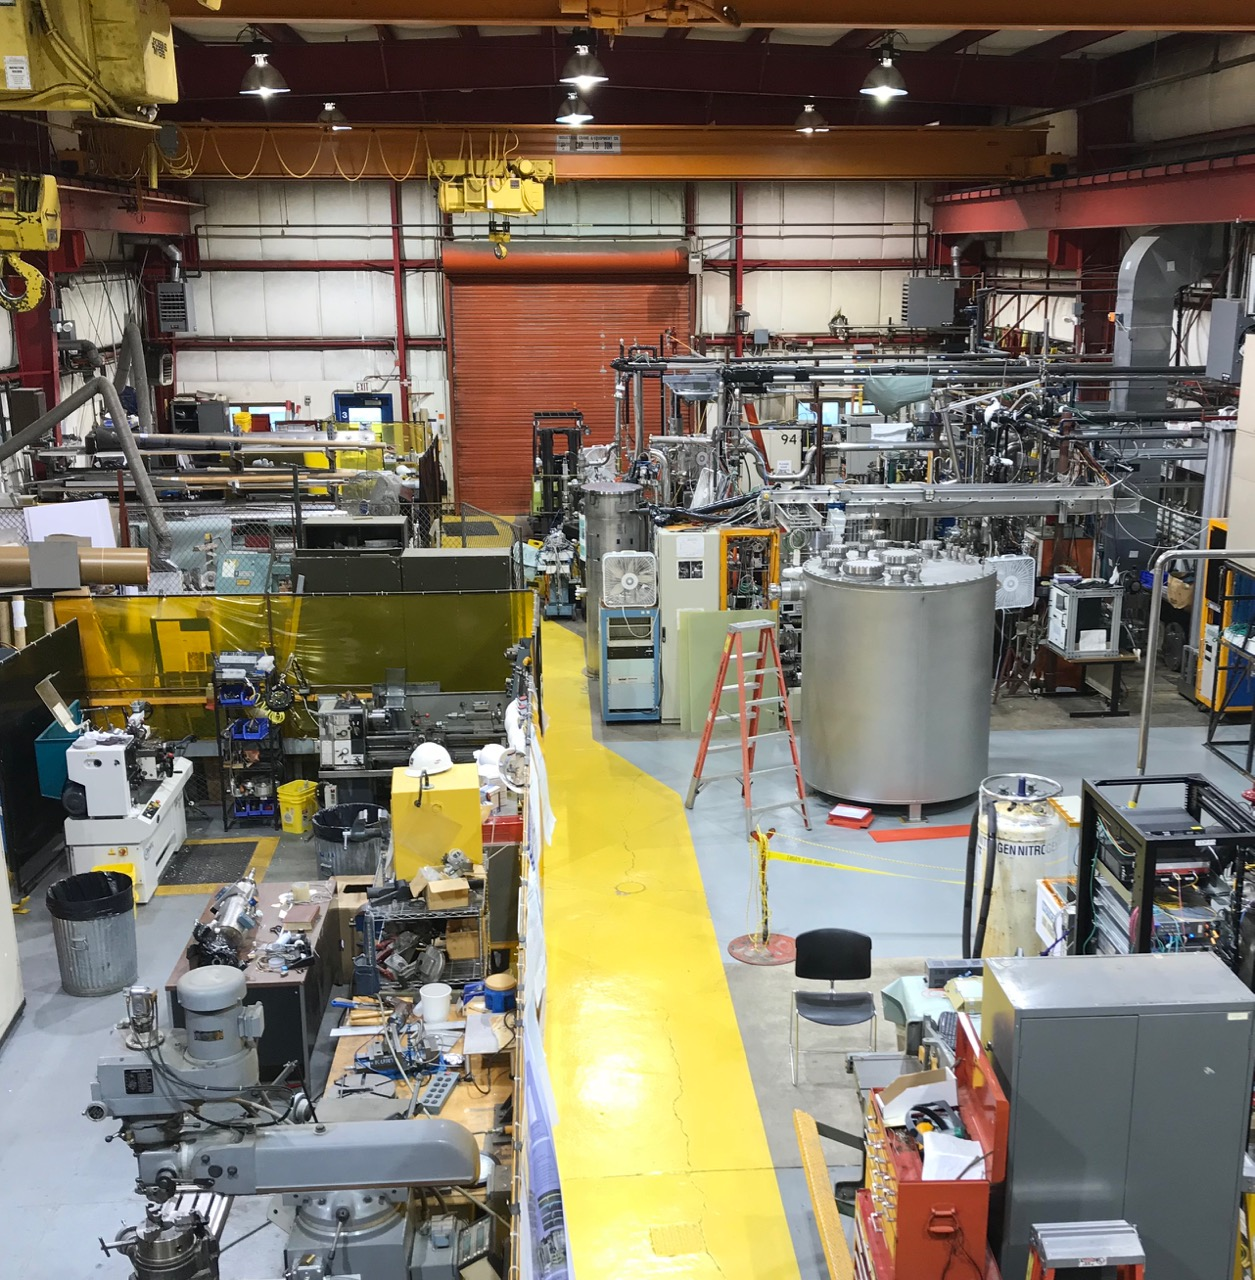
\includegraphics[width=0.9\textwidth]{cisc_PAB_photo.jpg}
%\end{dunefigure}

%\fixme{suggestion to remove this figure entirely or crop it to upper right and adjust text. It doesn't clarify anything. Tim and Anne  GLENN AND CARMEN TO CHECK}

The PAB facility at \fnal houses the ICEBERG \SI {3000} {liter} cryostat which enables fast turnaround testing for the \dword{dune} \dword{ce}. 

The PAB facility also includes TallBo (\SI {450} {liter}), Blanche (\SI {500} {liter}), and Luke (\SI {250} {liter}) cryostats. %All these cryostats are available for outside use.
In the recent past, Blanche has been used for \dword{hv} studies, TallBo for \dword{pd} studies, and Luke for the material test stand work. These studies have contributed to the design and testing of  \dword{pdsp} components.

\subsection{Validation in ProtoDUNE}
\label{sec:pdsp-cryo-valid}

Design validation and testing of many planned \dword{cisc} systems for
the \dword{spmod} will be done using the data from
\dword{pdsp} and \dword{pddp} as discussed below.

\begin{itemize}
	\item {\bf Level Meters:} The same differential pressure level meters
	      which are already validated in \dword{pdsp} will be used in \dword{spmod}. The same capacitive level meters currently used in
	      \dword{pddp} will be used in the \dword{spmod}. These will be
	      validated in the upcoming \dword{pddp} run.
	\item {\bf Pressure Meters (GAr):} Same high precision pressure sensors which are already validated in \dword{pdsp} will be used in \dword{sp} \dword{fd}.
	\item {\bf Gas Analyzers:} The same gas analyzers currently used in
	      \dword{pdsp} will be used in the \dword{spmod} so they have already
	      been validated.
	\item {\bf High precision thermometer arrays in \lar:} The static
	      and dynamic T-gradient thermometers discussed in the previous sections are validated using \dword{pdsp} data.
	\item {\bf Purity monitors:} The same purity monitor basic design used in \dword{pdsp} will be used in the \dword{fd} \dword{spmod}. \dword{pdsp} and \dword{pddp} run 2 phase provides opportunities to
	      test any improvements to the design.
	\item {\bf Cameras:} various types of cameras are being actively
	      developed in both \dword{pdsp} and \dword{pddp} so the validation of
	      designs will be performed both at \dword{pdsp} and \dword{pddp}. Future
	      improvements can be tested in \dword{pdsp} and \dword{pddp} run 2 phase
	      at CERN.
\end{itemize}


%%%%%%%%
\section{Slow Controls}
% same for SP and DP

The slow controls system collects, archives, and displays data from
a broad variety of sources and provides real-time status, alarms, and warnings for detector operators. Slow controls also provides control for %some detector components of the detector systems 
items such as \dword{hv} systems, \dword{tpc} electronics, and \dword{pd} systems. Data is acquired via network interfaces.  Figure~\ref{fig:gen-slow-controls-diagram} shows connections between major parts of the slow controls system and other systems. %Hardware, infrastructure, and software are the three main components of the slow controls system. %, each of which are described in this section.

\begin{dunefigure}[Slow controls connections and data]{fig:gen-slow-controls-diagram}
{Typical slow controls system connections and data flow}
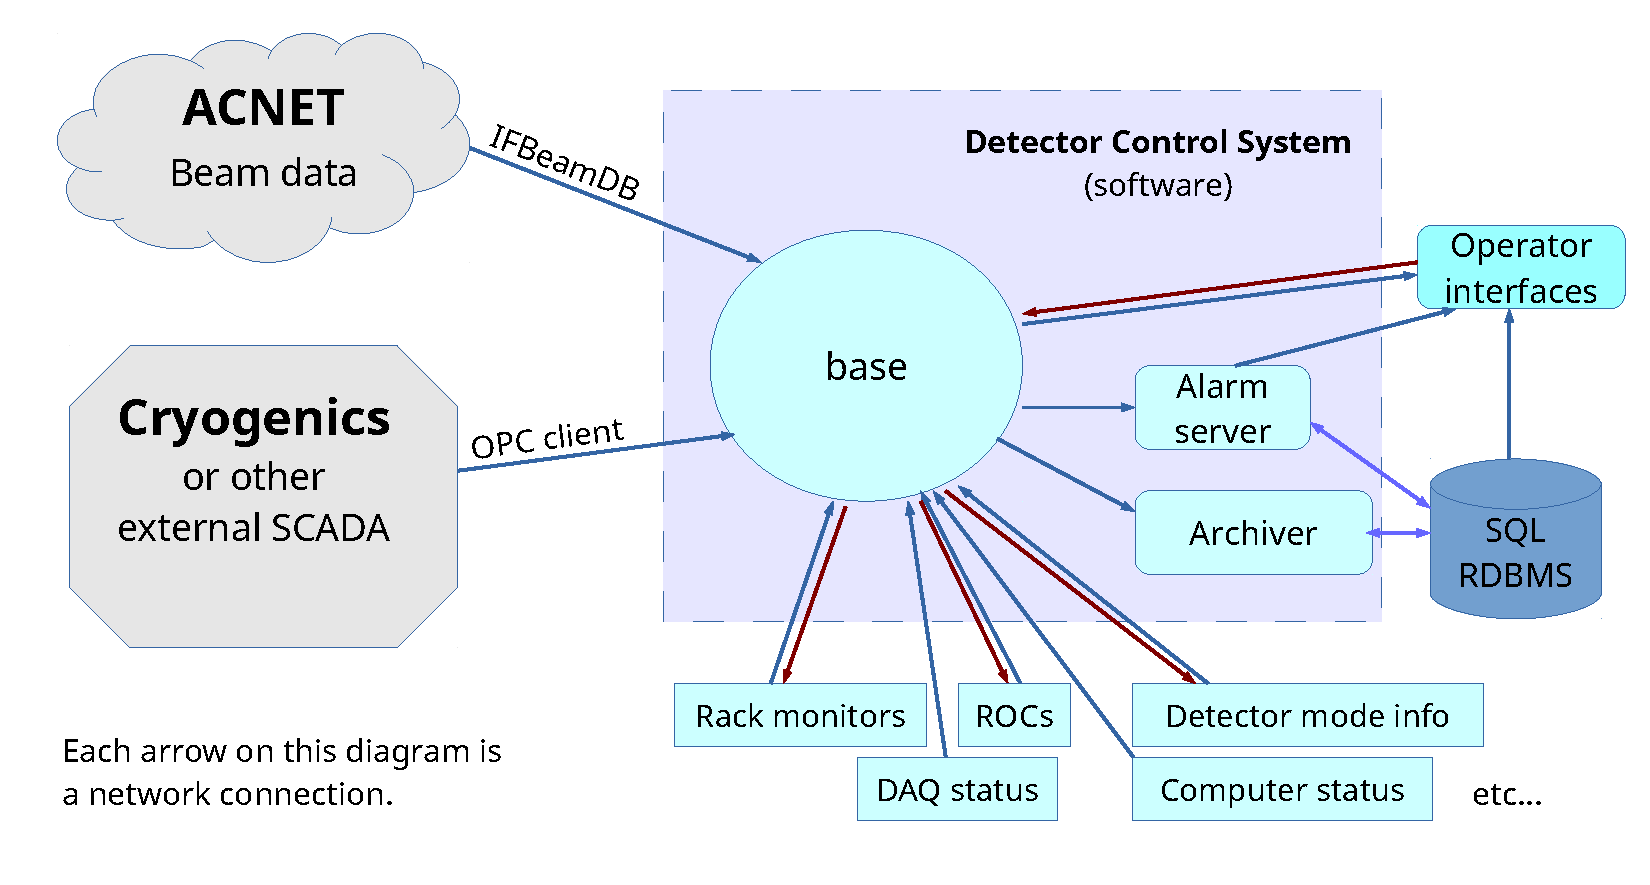
\includegraphics[width=0.7\textwidth]{cisc_slow-controls-diagram}
\end{dunefigure}

The \dword{pdsp} detector control system\cite{pdspdcs_proc} fully met its operational requirements. %the requirements for operating \dword{pdsp}. 
Section~\ref{sec:cisc-slow-control-pdsp} provides a short description of the \dword{pdsp} slow controls and its performance.

%%%%%%%%%%%%%%%%%%%%%%%%%%%%%%%%%%%
 \subsection{Slow Controls Hardware}
\label{sec:fdgen-slow-cryo-hdwr}

%A modest amount of dedicated hardware is envisioned for 
Slow controls is expected to need a modest amount of dedicated hardware, largely for rack monitoring,  %Additionally, slow controls will always 
and a small amount of dedicated network and
computing hardware. % as described below. 
Slow controls also relies on common
infrastructure as described in
Section~\ref{sec:fdgen-slow-cryo-slow-infra}.

%%%%%%%%%%%%%%%%%
\subsubsection{Dedicated Monitoring Hardware}

Every rack (including those in the \dword{cuc}) should have dedicated hardware to monitor rack parameters like rack protection system, rack fans, rack air temperatures, thermal interlocks with power supplies, and any interlock bit status monitoring needed for the racks. For the racks in the \dword{cuc} server room, this functionality is built into the proposed water cooled racks, as already in place at \dword{protodune}.  For the racks on the detector itself, the current plan is to design and install a custom-built 1U rack-mount enclosure containing a single-board computer to control and monitor various rack parameters. Such a system has been successfully used in MicroBooNE. The design is being improved for the short-baseline near detector (SBND) experiment (see Figure~\ref{fig:slow-controls-rack-box}). Other slow controls hardware includes interfacing cables like adapters for communication and debugging and other specialized cables like GPIB or National Instruments cables. The cable requirements must be determined in consultation with other groups once hardware choices for various systems are finalized.

\begin{dunefigure}[Rack monitoring box prototype for the SBND; based on MicroBooNE design]{fig:slow-controls-rack-box}
{Rack monitoring box prototype in development for the short-baseline near detector (SBND) experiment based on the original design from MicroBooNE.}
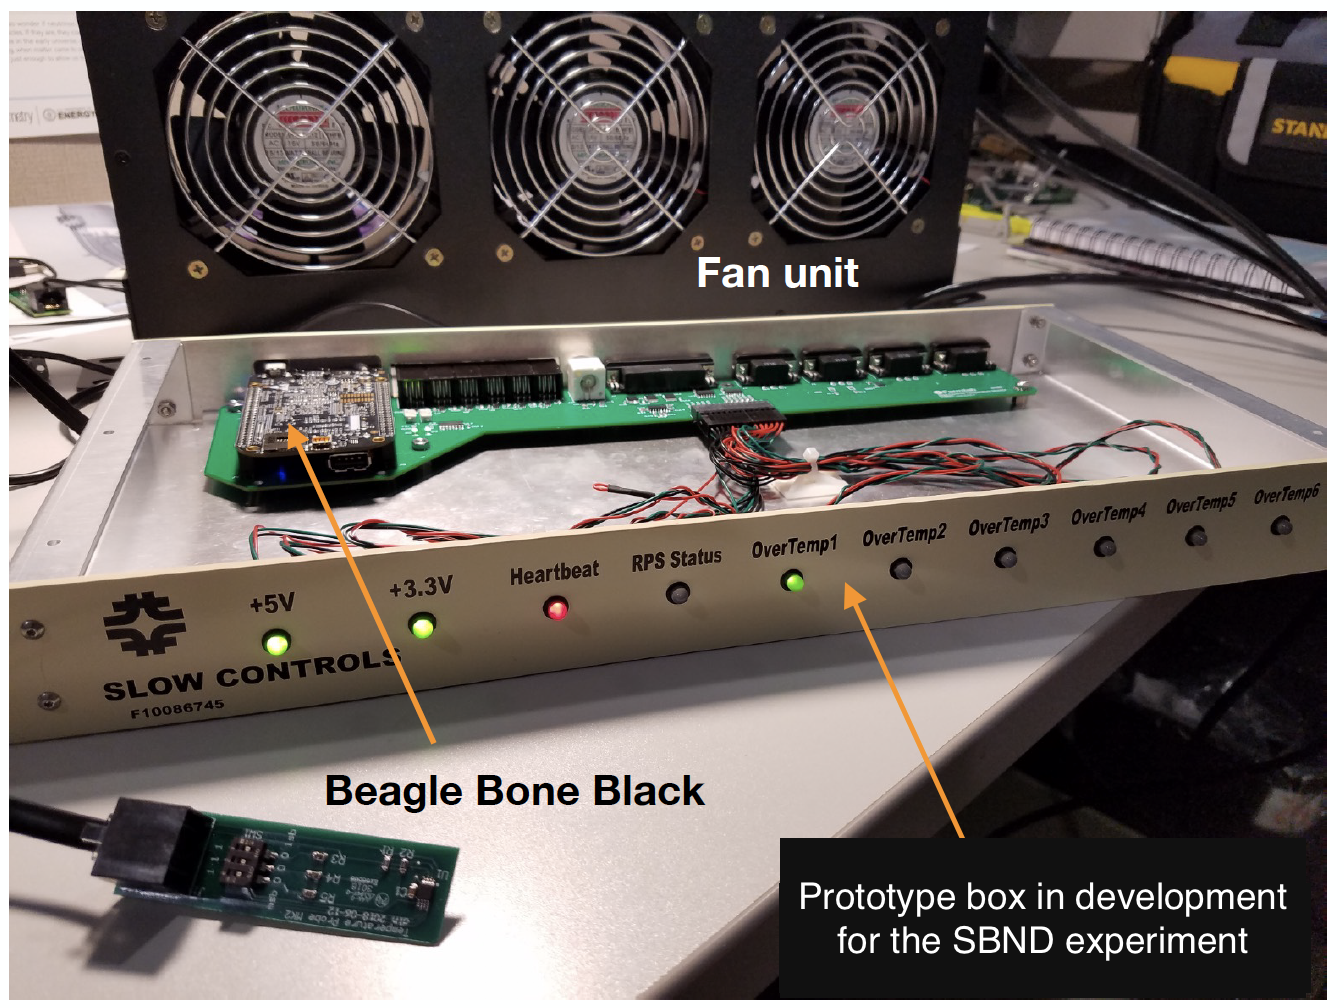
\includegraphics[width=0.6\textwidth]{cisc-slow-controls-rackbox.png}
\end{dunefigure}


% % % % Alec
\subsubsection{Slow Controls Network Hardware}
\label{sec:fdgen-slow-cryo-slow-network}
The slow controls data originates from the cryogenic instrumentation and from other systems as listed in Table~\ref{tab:gen-slow-quant}. This data is collected by software running on servers
(Section~\ref{sec:fdgen-slow-cryo-slow-compute})
housed in the underground data room in the \dword{cuc},
where data is archived in a central \dword{cisc} database.
The instrumentation data is transported over
conventional network hardware from any sensors located in the cryogenic
plant.  However, the readouts that are in the racks on top of the
cryostats must be cautious about grounding and noise.  Therefore, each
rack on the cryostat has a small network switch that sends
any network traffic from that rack to the \dword{cuc} via a fiber transponder.
This is the only network hardware specific to slow controls and will be provided by %the laboratory's
\surf{}'s  
general computing infrastructure. % managed by project \dword{tc}. 
The network infrastructure requirements are described in
Section~\ref{sec:fdgen-slow-cryo-slow-infra}.

% % % % Alec
\subsubsection{Slow Controls Computing Hardware}
\label{sec:fdgen-slow-cryo-slow-compute}
Two servers (a primary server and a replicated backup) suitable for the relational database discussed
in Section~\ref{sec:fdgen-slow-cryo-sw} are located in the \dword{cuc} data
room, with an additional
two servers to service the \dword{fe} monitoring interface; such service would include assembling dynamic \dword{cisc} monitoring web pages from adjacent
databases.  Another server will be needed to run back-end I/O.  Any special purpose software, such as iFix used by the cryogenics experts, would
also run here. One or two additional servers should accommodate these programs.
% (The exact number of iFix machines will be determined based
% on input from the LBNF cryogenics experts.)
Replicating this setup on a per-module basis would make commissioning and independent operation easier, accommodate different module
design (and the resulting differences in database tables), and ensure
sufficient capacity.  These four sets of networking hardware would fit tightly into one rack or very comfortably into two. Using the requirements from \dword{cisc}, the \dword{daq} consortium will provide the needed cost 
%estimates 
for servers and racks. 

% % % % Alec and Sowjanya
%% \subsubsection{Slow Controls Signal Processing Hardware}
%% Dropped because slow controls scope is defined not to include it.
%% (Signal processing should be within the scope of the hardware
%% generating the signal -- and so should digitization, for that matter.)
%%
%% N.B. The ``laundry list of Things to Be Monitored'' is in
%% \ref{sec:fdgen-slow-cryo-quant}



%%%%%%%%%%%%%%%%%%%%%%%%%%%%%%%%%%%
% Alec
\subsection{Slow Controls Infrastructure}
\label{sec:fdgen-slow-cryo-slow-infra}

The data rate will be in the range of tens of kilobytes per second, given the total number of slow controls quantities and the update rate  
(see Section~\ref{sec:fdgen-slow-cryo-quant}), placing minimal demands
on local network infrastructure.
Network traffic out of \surf to \fnal will primarily be database calls
to the central \dword{cisc} database, either from monitoring applications or from
database replication to the offline version of the \dword{cisc} database.  This
traffic requires little bandwidth, so the proposed general purpose
links both out of the %mine 
underground area at \surf and back to \fnal can accommodate the traffic.

Up to two racks of space and appropriate power and cooling are
available in the \dshort{cuc}'s \dword{daq} server room for \dword{cisc} use. This is ample space as described in Section
\ref{sec:fdgen-slow-cryo-slow-compute}.
%\fixme{[Carmen] Check Anne modification. reference to section \ref{sec:fdgen-slow-cryo-slow-compute} has been removed}
%Somewhat less space than that is currently envisioned, as described in Section
%\ref{sec:fdgen-slow-cryo-slow-compute}.


%%%%%%%%%%%%%%%%%%%%%%%%%%%%%%%%%%
% Sowjanya
\subsection{Slow Controls Software}
\label{sec:fdgen-slow-cryo-sw}
%\fixme{SG: does this need any updating based on presentations from Glenn/Alec at the Sept. Collaboration meeting? GAHS: I don't think so. PDSP DCS citation added. SG: okay, taking it out. I agree.}
% same for SP and DP

To provide complete monitoring and control of detector subsystems, the slow controls software includes
%
\begin{itemize}
 \item the control systems base that performs input and output operations
  and defines processing logic, scan conditions, and alarm conditions;
 \item an alarm server that monitors all channels and sends alarm
  messages to operators;
 \item a data archiver that performs automatic sampling and storage of
  values for history tracking; and 
 \item an integrated operator interface that provides display panels for
  controls and monitoring.
\end{itemize}

An additional requirement for the software is the capability to 
interface indirectly with external systems (e.g., cryogenics control
system) and databases (e.g., beam database) to export data into
slow controls process variables (or channels) for archiving and status
displays. This allows us to integrate displays and warnings into one
system for the experiment operators, and %to provide 
provides integrated
archiving for sampled data in the archived database. As one possibility, an input output controller (IOC) running on a central \dword{daq}
server could provide soft channels for these data.
Figure~\ref{fig:gen-slow-controls-diagram} shows a typical workflow of a
slow controls system.

The key features of the software require highly evolved software designed to manage real-time data exchange, scalable
to hundreds of thousands of channels sampled at intervals of hours to seconds as needed. The software
must be well documented, supported, and reliable. The base
software must also allow easy access to any channel by name. The
archiver software must allow data storage in an SQL database with
adjustable rates and thresholds so data
for any channel can be easily retrieved using channel name and time range. Among other key
features, the alarm server software must remember the state, support an
arbitrary number of clients, and provide logic for delayed alarms and
acknowledging alarms. A standard naming
convention for channels will be part of the software to help handle large
numbers of channels and subsystems.

%\fixme{CP: Paragraph below modified to explain the baseline software here}
The \dword{pdsp} detector control system software \cite{pdspdcs_proc} (NP04-DCS) provides a prototype for %this required 
the \dword{fd} slow
controls software. In NP04-DCS, the unified control system base is WinCC OA \cite{winccoa}, a
commercial toolkit used extensively at CERN, with device interfaces
supported using several standardized interface protocols. A more detailed description is in Section~\ref{sec:cisc-slow-control-pdsp} below.

%provides a prototype for this required \dword{fd} slow
%controls software, as described in Section~\ref{sec:cisc-slow-control-pdsp} below.

%%%%%%%%%%%%%%%%%%%%%%%%%%%%%%%%%%
% Ed T
\subsection{Slow Controls Quantities}
\label{sec:fdgen-slow-cryo-quant}

% starter text from Glenn

The final set of quantities to monitor will ultimately be determined
by the subsystems being monitored, documented in
appropriate  interface control documents (ICDs), and continually revised based on operational
experience.  The total number of quantities to monitor has been roughly estimated by taking the total number monitored
in \dword{pdsp}\cite{pdspdcs_proc}, 7595 as of Nov. 19, 2018, and scaling by the detector length and the number of planes, giving approximately 150,000 per \dword{detmodule}.% in the range of \numrange{140}{190} thousand. % let's keep just 1 digit of precision to be safe [glenn]
Quantities should update on average no more than once per minute.
Transmitting a single update for each channel at that rate translates to a few thousand updates per second, or a few tens of thousands of bytes per second. While this is not a significant load on a network with an efficient slow controls protocol, it would correspond to approximately 1~TB per year if every timestamp and value were stored.

The subsystems
to be monitored include the %detector 
cryogenic instrumentation
described in this chapter, the other detector systems, and relevant
infrastructure and external devices. Table \ref{tab:gen-slow-quant}
lists the quantities expected from each system.

\begin{dunetable}
[Slow controls quantities]
{p{0.3\textwidth}p{0.6\textwidth}}
{tab:gen-slow-quant}
{Slow controls quantities}
System & Quantities \\ \toprowrule
\multicolumn{2}{l}{\bf Detector cryogenic instrumentation } \\ \specialrule{1.5pt}{1pt}{1pt}
Purity monitors & anode and cathode charge, bias voltage and current, flash lamp status, calculated electron lifetime \\ \colhline
Thermometers & temperature, position of dynamic thermometers \\ \colhline
Liquid level & liquid level \\ \colhline
Gas analyzers & purity level readings \\ \colhline
Pressure meters & pressure readings \\ \colhline
Cameras & camera voltage and current draw, temperature, heater current and voltage, lighting current and voltage \\ \toprowrule
\multicolumn{2}{l}{\bf Other detector systems } \\ \specialrule{1.5pt}{1pt}{1pt}
Cryogenic internal piping & \fdth gas purge flow and temperature \\ \colhline
\dword{hv} systems & drift \dword{hv} voltage and current, end-of-field cage current and bias voltage, electron diverter bias, ground plane currents \\ \colhline
TPC electronics & voltage and current to electronics \\ \colhline
\dword{pd} & voltage and current for photodetectors and electronics \\ \colhline
\dword{daq} & warm electronics currents and voltages, run status, \dword{daq} buffer sizes, trigger rates, data rates, GPS status, computer and disk health status, other health metrics as defined by \dword{daq} group \\ \colhline
\dword{crp} / \dword{apa} & bias voltages and currents \\ \toprowrule
\multicolumn{2}{l}{\bf Infrastructure and external systems } \\ \specialrule{1.5pt}{1pt}{1pt}
Cryogenics (external) & status of pumps, flow rates, inlet and return temperature and pressure (via OPC or similar SCADA interface) \\ \colhline
Beam status & protons on target, rate, target steering, beam pulse timing (via IFBeamDB) \\ \colhline
Near detector & near detector run status (through common slow controls database) \\ \colhline
Rack power and status & power distribution unit current and voltage, air temperature, fan status if applicable, interlock status \\ \colhline
\multicolumn{2}{l}{\bf Detector calibration systems } \\ \specialrule{1.5pt}{1pt}{1pt}
Laser & laser power, temperature, operation modes, other system status as defined by calibration group\\ \colhline
External neutron source  & safety interlock status, power supply monitoring, other system status as defined by calibration group \\ \colhline
External radioactive source & system status as defined by calibration group\\
\end{dunetable}

%%%%%%%%%%%%%%%%%%%%%%%%%%%%%%%%%%
% Sowjanya and Anselmo
\subsection{Local Integration}
\label{sec:fdgen-slow-cryo-slow-loc-integ}

% This subsection is redundant with ``interfaces'', but there is a WBS
% section with the name ``Local integration'' that contains only interfaces,
% so keeping the subsection and adding some text saying what it is.

The local integration of the slow controls consists entirely of software
and network interfaces with systems outside of the scope of the \dword{detmodule}.
This includes the following:
\begin{itemize}
\item readings from the LBNF-managed external cryogenics systems, for status of pumps, flow rates, inlet, and return temperature and pressure, which are implemented via OPC or a similar SCADA interface;
\item beam status, such as protons-on-target, rate, target steering, and beam pulse timing, which are retrieved via IFBeamDB; and 
\item near detector status, which can be retrieved from a common slow controls database.
\end{itemize}
%
Integration occurs after both the slow controls and non-detector
systems are in place.  The LBNF-\dword{cisc} interface is managed by the
cryogenics systems working group in \dword{cisc} as described in Section~\ref{sec:cisc-slow-controls-org}, which includes members from both \dword{cisc} and \dword{lbnf}. 
The IFBeamDB interface for slow controls is already well established in \microboone, \nova, and other \fnal experiments. An internal near-detector--\dword{fd} working group can be established 
to coordinate detector status exchange between the near and far sites.

%%%%%%%%%%%%%
\subsection{Validation in \dword{protodune}}
\label{sec:cisc-slow-control-pdsp}

\begin{dunefigure}[Diagram of the \dword{pdsp} control system topology]{fig:cisc-NP04-DCS-topology}
{Diagram of the \dword{pdsp} control system (NP04 DCS) topology, from \cite{pdspdcs_proc}.}
% Figure cannot be scaled down smaller than height=0.9\textheight,width=0.95\textwidth without making text unreadable. Even at this scale, the largest text on figure is 75% of the caption text font size. Authors of the NP04-DCS paper are making a new figure, just not ready for 1st TDR draft. [Glenn]
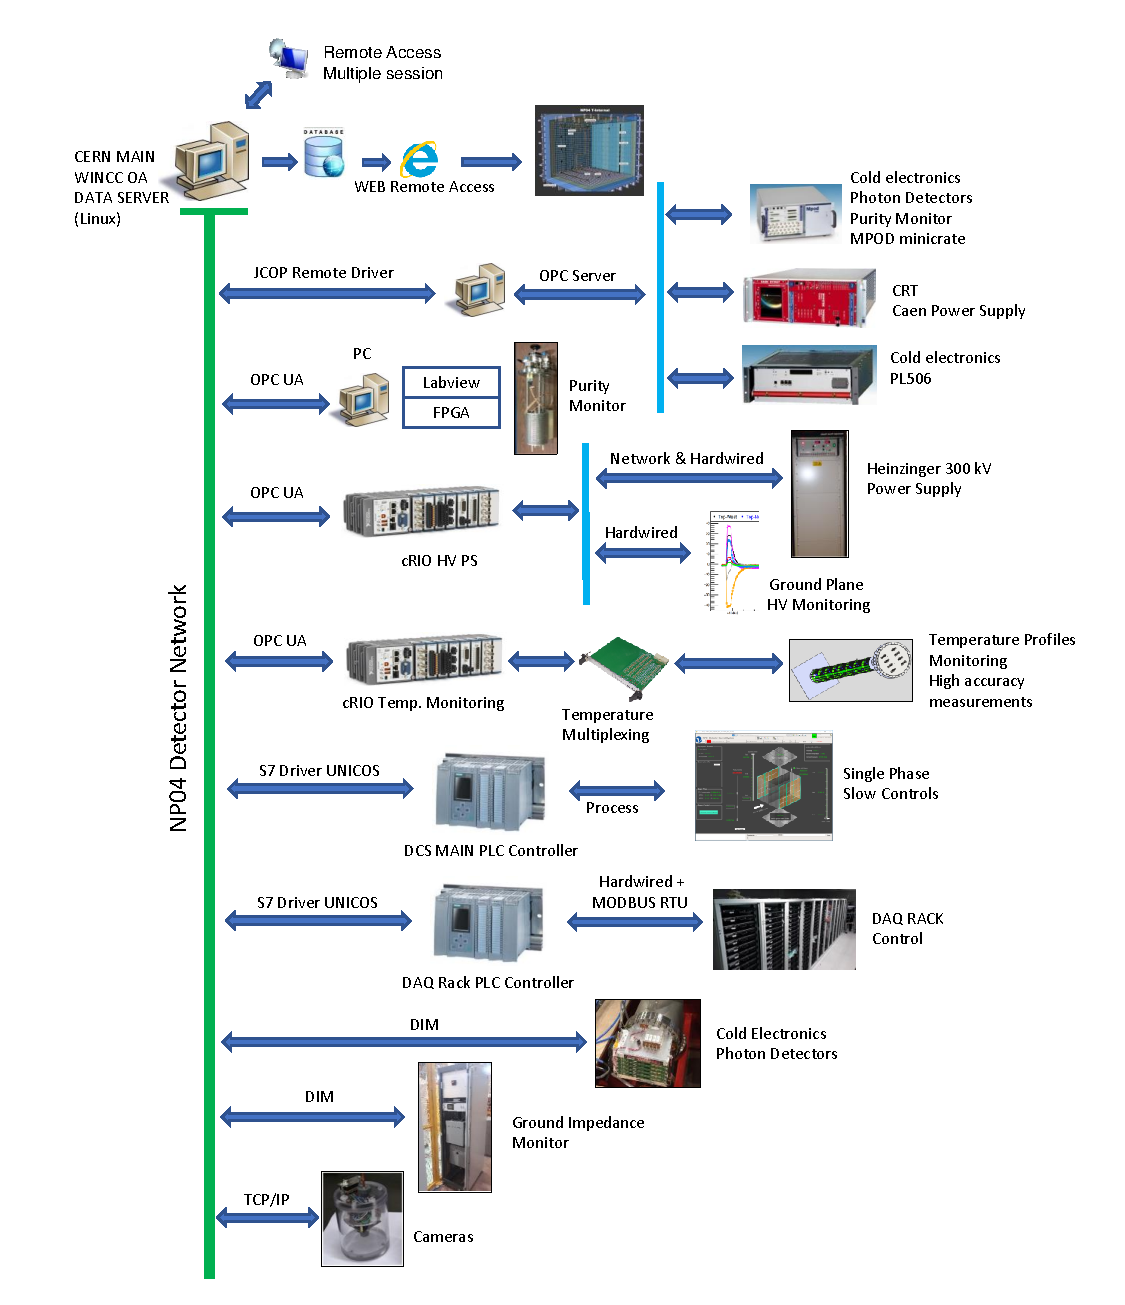
\includegraphics[height=0.9\textheight,width=0.95\textwidth,keepaspectratio]{NP04-DCS_arch_vert}
\end{dunefigure}

The \dword{pdsp} detector control system (also known as NP04-DCS) met
all requirements for operation in September 2018, as
described in \cite{pdspdcs_proc}.  Those requirements are
nearly identical to those for the \dword{spmod} other than
total channel count. Of particular note, the NP04-DCS unified a heterogenous set of devices and data sources
through multiple protocols into a
single control system, as illustrated in
Figure~\ref{fig:cisc-NP04-DCS-topology}. In addition to what
the figure shows, data was also acquired from external cryogenic and beam
systems.  The topology and data flow of the system matches the general
shape shown in Figure~\ref{fig:gen-slow-controls-diagram}. In NP04-DCS,
the unified control system base is a
commercial toolkit (WinCC OA) supported by CERN.
%used extensively at CERN, with device interfaces
%supported using several standardized interface protocols.

As noted in sections \ref{sec:fdgen-slow-cryo-sw} and \ref{sec:fdgen-slow-cryo-quant},
the %\dword{dune} 
\dword{spmod} slow control system will produce massive amounts of
data, requiring a sizable database to store the value history and
allow efficient data retrieval. Individually adjustable rates and
thresholds for each channel are key in keeping this database
manageable. The \dword{pdsp} operations provided not only a test of
these features as implemented in the NP04 DCS, but also insight into
reasonable values for these archiving parameters for each system.


%%%%%%%%
\section{Organization and Management}
\label{sec:cisc-slow-controls-org}

The organization of the CISC consortium is shown in
 Figure~\ref{fig:gen-slow-cryo-org}. The CISC consortium board currently comprises institutional representatives from 18 institutes as shown in Table~\ref{tab:gen-slow-cryo-org}. The consortium leader is the spokesperson for the consortium and responsible for the overall scientific program and managing the group. The technical leader of the consortium is responsible for managing the project for the group. Currently, the
consortium has five working groups:
\begin{description}
 \item[Cryogenics Systems] gas analyzers and liquid level
  monitors; \dword{cfd} simulations
 \item[Argon Instrumentation] purity monitors, thermometers, pressure meters, capacitive level meters, cameras and light emitting system, and instrumentation test facility; feedthroughs; \efield simulations; instrumentation precision studies; \dword{protodune} data analysis coordination and validation 
 \item [Slow Controls Base Software and Databases]  base I/O software, alarms and archiving databases, and monitoring tools;
   variable naming conventions and slow controls quantities
 \item [Slow Controls Detector System Interfaces] signal processing software and hardware interfaces (e.g., power supplies); firmware; rack hardware and infrastructure   
 \item [Slow Controls External Interfaces] interfaces with external detector systems (e.g., cryogenics system, beam, facilities, \dword{daq}, near detector status)
\end{description}

\begin{dunefigure}[CISC consortium organization]{fig:gen-slow-cryo-org}
{CISC Consortium organizational chart}
\includegraphics[width=0.8\textwidth]{graphics/CISC_Org_9Apr2019_zoomedin.png}
\end{dunefigure}

\begin{dunetable}
[CISC Consortium Institutions]
%{p{0.43\textwidth}p{0.12\textwidth}p{0.22\textwidth}}
{lc}
{tab:gen-slow-cryo-org}
{Current \dword{cisc} Consortium Board Members and their institutional affiliations}
Member Institute                         &  Country       \\%  &  Consortium Board Representative \\ \toprowrule
CIEMAT                                   &  Spain         %  &  Ines Gil Botella 
\\ \colhline
Instituto de Fisica Corpuscular (IFIC)          &  Spain          % &  Anselmo Cervera 
\\ \colhline
University of Warwick                    &  UK % &  Gary Barker 
\\ \colhline
University College London (UCL)             &  UK  %&  Mario Campanelli 
\\ \colhline
Argonne National Lab (ANL)                     &  USA             %&  Jim Grudzinski 
\\ \colhline
Brookhaven National Lab (BNL)                  &  USA            % &  Jim Stewart
\\ \colhline
University of California, Irvine (UCI)        &  USA            % &  Jianming Bian 
\\ \colhline
Drexel University                        &  USA           %  &  Charles Lane 
\\ \colhline
Fermi National Accelerator Lab (\fnal)           &  USA           %  &  Alan Hahn
\\ \colhline
University of Hawaii                     &  USA            % &  Jelena Maricic 
\\ \colhline
University of Houston                    &  USA           %  &  Andrew Renshaw 
\\ \colhline
Idaho State University (ISU)                   &  USA           %  &  Ed Tatar 
\\ \colhline
Kansas State University (KSU)                  &  USA            % &  Glenn Horton-Smith 
\\ \colhline
University of Minnesota, Duluth (UMD)         &  USA            % &  Alec Habig 
\\ \colhline
Notre Dame University                    &  USA            % &  John LoSecco 
\\ \colhline
South Dakota State University (SDSU)           &  USA            % &  Stephen Gent
\\ \colhline
University of Tennessee at Knoxville (UTK)     &  USA           %  &  Sowjanya Gollapinni 
\\ \colhline
Virginia Tech (VT)                            &	USA	           % &  Camillo Mariani
\\	\colhline
	Boston University (BU)			      & USA % & Edward Kearns
\\
\end{dunetable}

Moreover, because the \dword{cisc} consortium broadly interacts with other groups, liaisons have been named as shown in Figure~\ref{fig:gen-slow-cryo-org}. 
A short-term task force was recently formed to explore the need for cryogenic modeling for the consortium. A work plan for \dword{cfd} simulations for both \dword{protodune} and \dword{fd} was developed based on input from the task force. The \dword{tdr} editors are responsible for the overall editing and delivery of the \dword{tdr} document. Currently, members from new institutes are added to the consortium based on consensus from the consortium board members following an expression of interest petition from the new institute.

\subsection{Institutional Responsibilities}

The \dword{cisc} %slow controls and cryogenic instrumentation 
will be a joint effort for \single and \dual. A single slow controls system will be implemented to serve both the \dword{spmod} and the \dword{dpmod}.

Design and installation of cryogenic systems (e.g., gas analyzers, liquid level monitoring) will be coordinated with \dword{lbnf}, with the consortium providing resources and effort, and expertise provided by \dword{lbnf}. \dword{protodune} designs for \lar instrumentation (e.g., purity monitors, thermometers, cameras, test facility) will be the basis for \dword{detmodule} designs. Design validation, testing, calibration, and performance will be evaluated through \dword{protodune} data.

Following the conceptual funding model envisioned for the consortium, various responsibilities have been distributed across institutions within the consortium. At this stage of the project, firm funding decisions are not made yet.
%At this stage of the project, these should be considered as ``aspirational`` responsibilities until firm funding decisions are made.
Table~\ref{tab:cisc-inst-resp} shows the current institutional responsibilities for primary \dword{cisc} subsystems. Only lead institutes are listed in the table for a given effort. For physics and simulations studies, and validation efforts with \dword{protodune}, a number of institutes are involved. A detailed list of tasks and institutional responsibilities are presented in~\cite{bib:docdb5609}.

\begin{dunetable}
[Institutional responsibilities in the CISC consortium ]
{p{0.4\textwidth}p{0.45\textwidth}}
{tab:cisc-inst-resp}
{Institutional responsibilities in the \dword{cisc} consortium}
CISC Sub-system     &  Institutional Responsibility \\ \toprowrule
Purity Monitors          &  UCI, Houston \\ \colhline
Static T-gradient monitors     &  IFIC \\ \colhline
Dynamic T-gradient monitors & Hawaii \\ \colhline
Individual Sensors & IFIC \\ \colhline
Readout System for Thermometers & IFIC, Hawaii, CIEMAT \\ \colhline
Pressure Meters & UTK \\ \colhline
Cold Cameras & KSU, BNL \\ \colhline
Warm Cameras & KSU, BNL \\ \colhline
Light-emitting System (for cameras) & Drexel \\ \colhline
Gas Analyzers & FNAL, \dword{lbnf} \\ \colhline
Differential Pressure Level Meters & \dword{lbnf} \\ \colhline
Capacitive Level Meters & Notre Dame \\ \colhline
Cryogenic Instrumentation Test Facility & FNAL, ANL \\ \colhline
\dword{cfd} Simulations & SDSU, ANL \\ \colhline
Other Simulation \& Validation Studies & Number of Institutes \\ \colhline
Slow Controls Hardware & UMD, UTK, Drexel\\ \colhline
Slow Controls Infrastructure & UMD, UTK\\ \colhline
Slow Controls Base Software & KSU, UTK, BU, Drexel, Warwick, ANL, IFIC\\ \colhline 
Slow Controls Signal Processing & A number of institutes \\ \colhline
Slow Controls External Interfaces & VT, UTK, UMD \\
\end{dunetable}

\subsection{Cost and Labor}

Table \ref{tab:cisc-cost} shows the current cost estimates for the \dword{cisc} subsystems. It also shows the quantity associated with each subsystem and a brief description of what is included in the cost estimate. The cost estimates only include materials and supplies (M\&S) and packing and shipping, but not labor and travel costs. Labor costs depend on personnel category (e.g., faculty, student, technician, post-doc, engineer) and vary by region and institution, so costs are quantified using labor hours needed to fulfill a given task. Table~\ref{tab:cisc-labor} provides estimates of labor hours for each subsystem, for a total of \num{95010} labor hours for all \dword{cisc} tasks. 

\fixme{3/25 Anne: Cost and labor hour tables will be automated in early April. Info to come.}

\fixme{Commenting out the cost column for submission to LBNC per Tim. Anne}
\begin{comment}
\begin{dunetable}
[CISC Cost]
{p{0.3\textwidth}p{0.08\textwidth}p{0.1\textwidth}p{0.45\textwidth}}
{tab:cisc-cost}
{Cost estimates of the different CISC subsystems. All cost estimates include pacing and shipping costs.}
System                         & Quantity & Cost & Description  \\ \toprowrule
Purity monitors                & 10 & \$309,400 & Includes material cost, PC, flanges, mounting structure  \\ \colhline
Static T-gradient monitors     & 6 & \$88,340 & Includes cables, sensors and connectors, support structure, flanges \\ \colhline
Precision individual temperature sensors & 130 & \$51,512 & Includes cables, sensors and connectors, support structure, flanges \\ \colhline
Standard individual temperature sensors & 35 & \$12,615 & Includes cables, sensors and connectors, support structure, flanges \\ \colhline
Dynamic T-gradient monitors    & 2 & \$108,060 & Includes cables, sensors, motor drive, flanges, sensor holders \\ \colhline
Pressure Meters (GAr) & 6 & - & Includes pressure meters and flanges \\ \colhline
Warm cameras                   & 3 & \$294,775 & Includes material cost, computer, argon purge \& pressurization system, prototyping \& testing  \\ \colhline
Cold cameras                   & 12 & \$38,300  & Includes material cost, computer, minor jigs \& test boards \\ \colhline
Light system                   & 15 & \$4,900 & Cost of illuminator and light driver module    \\ \colhline
Gas analyzers                  & 1 & \$222,360 & Cost of gas analyzers and piping \& routing panel  \\ \colhline
Capacitive level meters        & 4 & \$19,018  & Cost of level meters and flanges   \\ \colhline
Cryogenics test facility       & 1 & \$62,000  & Material cost includes liquid argon costs for years 1 to 5 and minor fixture costs  \\ \colhline
Slow controls hardware         & - & \$78,970  & Cost of 6 servers, 0.5 rack, 126 rack monitoring boxes, and cables   \\ \colhline
Slow controls software         & - & \$1,500 & Includes cost of a laptop    \\ \colhline
\textbf{Total Cost}          &       & \textbf{\$1,291,750}& \\
\end{dunetable}
\end{comment}

\begin{dunetable}
[CISC Cost]
{p{0.3\textwidth}p{0.08\textwidth}p{0.1\textwidth}p{0.45\textwidth}}
{tab:cisc-cost}
{Cost estimates of the different CISC subsystems. All cost estimates include pacing and shipping costs.}
System                         & Quantity & Cost (under development) & Description  \\ \toprowrule
Purity monitors                & 10 & - & Includes material cost, PC, flanges, mounting structure  \\ \colhline
Static T-gradient monitors     & 6 & - & Includes cables, sensors and connectors, support structure, flanges \\ \colhline
Precision individual temperature sensors & 130 &- & Includes cables, sensors and connectors, support structure, flanges \\ \colhline
Standard individual temperature sensors & 35 & - & Includes cables, sensors and connectors, support structure, flanges \\ \colhline
Dynamic T-gradient monitors    & 2 & - & Includes cables, sensors, motor drive, flanges, sensor holders \\ \colhline
Warm cameras                   & 3 & - & Includes material cost, computer, argon purge \& pressurization system, prototyping \& testing  \\ \colhline
Cold cameras                   & 12 & - & Includes material cost, computer, minor jigs \& test boards \\ \colhline
Light system                   & 15 & - & Cost of illuminator and light driver module    \\ \colhline
Gas analyzers                  & 1 & - & Cost of gas analyzers and piping \& routing panel  \\ \colhline
Capacitive level meters        & 4 & \-  & Cost of level meters and flanges   \\ \colhline
Cryogenics test facility       & 1 &-  & Material cost includes liquid argon costs for years 1 to 5 and minor fixture costs  \\ \colhline
Slow controls hardware         & - & -  & Cost of 6 servers, 0.5 rack, 126 rack monitoring boxes, and cables   \\ \colhline
Slow controls software         & - & - & Includes cost of a laptop    \\ 
%\textbf{Total Cost}          &       & \textbf{\$1,291,750}& \\
\end{dunetable}

\fixme{removing hours from table because that implies costs. Per Tim. Anne}
\begin{comment}
\begin{dunetable}
[CISC labor]
{p{0.25\textwidth}p{0.15\textwidth}p{0.1\textwidth}p{0.08\textwidth}p{0.08\textwidth}p{0.1\textwidth}p{0.08\textwidth}}
{tab:cisc-labor}
{Estimate of labor hours for each category of personnel for different CISC subsystems. For slow controls software, the 884 technician hours comprises 442 hours from information technology professionals and 442 hours from scientific computing professionals.}
System  & Faculty/Scientist & Post-doc & Student & Engineer & Technician  &  \textbf{Total}\\ \toprowrule
& (hours) & (hours)& (hours)& (hours)& (hours)& (hours)\\ \toprowrule
Purity monitors & 5304& 5304& 5304& -& 1326 & \textbf{17238} \\ \colhline
Static T-gradient monitors & 3536& 1768& 2652&  442& 884& \textbf{9282} \\ \colhline
Individual temperature sensors & 3536& 1768& 2652&  442& 884& \textbf{9282} \\ \colhline
Dynamic T-gradient monitors & 3536& 3536& 3536&  354& 884& \textbf{11846} \\ \colhline
Warm cameras & 1768& 1768& 1768&  442& 737 & \textbf{6483}\\ \colhline
Cold cameras & 884& 1768& 1768& 100& 50& \textbf{4570}\\ \colhline
Light system & 884& - & 442 & - &20 & \textbf{1346}\\ \colhline
Gas analyzers & - & - & - &  320 & 480& \textbf{800}\\ \colhline
Level meters & - & - & - & 56 & - & \textbf{56}\\ \colhline
Cryogenic test facility & 1768& 2400& 2400& 180& 525& \textbf{7273}\\ \colhline
Slow controls hardware & 884 & 589& 884& 295 & 147& \textbf{2799}\\ \colhline
Slow controls software & 1768& 11492& - & 221 & 884& \textbf{14365}\\ \colhline
Physics \& simulation & 1768& 1768& 5604&  530 & - & \textbf{9670}\\ \colhline
\textbf{Total}  & \textbf{25636} & \textbf{32161}& \textbf{27010}& \textbf{3382}& \textbf{6821} & \textbf{95010}\\
\end{dunetable}
\end{comment}
\begin{dunetable}
[CISC labor]
{p{0.25\textwidth}p{0.15\textwidth}p{0.1\textwidth}p{0.08\textwidth}p{0.08\textwidth}p{0.1\textwidth}p{0.08\textwidth}}
{tab:cisc-labor}
{Estimate of labor hours for each category of personnel for different CISC subsystems. For slow controls software, the 884 technician hours comprises 442 hours from information technology professionals and 442 hours from scientific computing professionals.}
System  & Faculty/Scientist & Post-doc & Student & Engineer & Technician  &  \textbf{Total}\\ \toprowrule
& (hours) & (hours)& (hours)& (hours)& (hours)& (hours)\\ \toprowrule
Purity monitors & -& -& -& -& - & - \\ \colhline
Static T-gradient monitors & -& -& -& -& - & - \\ \colhline
Individual temperature sensors  & -& -& -& -& - & - \\ \colhline
Dynamic T-gradient monitors  & -& -& -& -& - & - \\ \colhline
Pressure Meters (GAr) & & & & & & \\ \colhline
Warm cameras  & -& -& -& -& - & - \\ \colhline
Cold cameras  & -& -& -& -& - & - \\ \colhline
Light system  & -& -& -& -& - & - \\ \colhline
Gas analyzers  & -& -& -& -& - & - \\ \colhline
Level meters  & -& -& -& -& - & - \\ \colhline
Cryogenic test facility  & -& -& -& -& - & - \\ \colhline
Slow controls hardware  & -& -& -& -& - & - \\ \colhline
Slow controls software  & -& -& -& -& - & - \\ \colhline
Physics \& simulation  & -& -& -& -& - & - \\ 
\end{dunetable}

\subsection{Schedule}

%\fixme{Anne: Please use this new template (\ref{tab:sp-cisc-sched}) (as of late March)}

%This is a standard table template for the TDR schedules.  It contains overall FD dates from Eric James as of March 2019 (orange) that are held in macros in the common/defs.tex file so that the TDR team can change them if needed. Please do not edit these lines! Please add your milestone dates to fit in with the overall FD schedule. 

\begin{dunetable}
[\dword{sp} \dword{cisc} Schedule]
{p{0.65\textwidth}p{0.25\textwidth}}
{tab:sp-cisc-sched}
{Key CISC construction schedule milestones leading to commissioning of the first FD module.}   
Milestone & Date (Month YYYY)   \\ \toprowrule
Technology Decision Dates &   September 2019   \\ \colhline
Final Design Review Dates &   November 2019   \\ \colhline
Start of module 0 component production for ProtoDUNE-II & March 2020  \\ \colhline
End of module 0 component production for ProtoDUNE-II & September 2020  \\ \colhline
\rowcolor{dunepeach} Start of \dword{pdsp}-II installation& \startpduneiispinstall      \\ \colhline
 \dword{prr} dates &  September 2021    \\ \colhline
Start procurement of \dword{cisc} hardware & December 2021 \\ \colhline
\rowcolor{dunepeach} Start of \dword{pddp}-II installation& \startpduneiidpinstall      \\ \colhline
Start of production of \dword{cisc} hardware & April 2022 \\ \colhline
\rowcolor{dunepeach}South Dakota Logistics Warehouse available& \sdlwavailable      \\ \colhline
\rowcolor{dunepeach}Beneficial occupancy of cavern 1 and \dword{cuc}& \cucbenocc      \\ \colhline
\rowcolor{dunepeach} \dword{cuc} counting room accessible& \accesscuccountrm      \\ \colhline
End of \dword{cisc} hardware production  &   July 2023   \\ \colhline
\rowcolor{dunepeach}Top of \dword{detmodule} \#1 cryostat accessible& \accesstopfirstcryo      \\ \colhline
%End of  (component 1) production  &      \\ \colhline
%... & ...                       \\ \colhline
Start integration of \dword{cisc} hardware in the cavern & March 2024   \\ \colhline
Installation of gas analyzers & April 2024\\ \colhline
Installation of support structure for all instrumentation devices &  May 2024 \\ \colhline
Installation of individual sensors, static T-gradient thermometers, and level meters & June 2024\\ \colhline
\rowcolor{dunepeach}Start of \dword{detmodule} \#1 TPC installation& \startfirsttpcinstall      \\ \colhline
All slow controls hardware, infrastructure, \& networking installed & February 2025\\ \colhline
Slow controls software for I/O, alarms, archiving, displays installed on production systems & May 2025 \\ \colhline
\rowcolor{dunepeach}End of \dword{detmodule} \#1 TPC installation& \firsttpcinstallend      \\ \colhline
Install dynamic T-gradient monitors, cameras, purity monitors & July 2025 \\\colhline
Install all feedthroughs for instrumentation devices & July 2025 \\ \colhline
Install slow control expert interfaces for all systems in time for testing & September 2025 \\ \colhline
Full slow controls systems commissioned and integrated into remote operations & July 2026 \\ 
\rowcolor{dunepeach}Top of 
\dword{detmodule} \#2 cryostat accessible& \accesstopsecondcryo      \\ \colhline
 \rowcolor{dunepeach}Start of \dword{detmodule} \#2 TPC installation& \startsecondtpcinstall      \\ \colhline
\rowcolor{dunepeach}End of \dword{detmodule} \#2 TPC installation& \secondtpcinstallend      \\ 
\end{dunetable}

Table \ref{tab:sp-cisc-sched} shows key construction milestones for the \dword{cisc} consortium leading to commissioning of the first \dword{fd} module. \dword{cisc} construction milestones align with the overall construction milestones of the first \dword{fd} module (highlighted in orange in the table). The technology design decisions for \dword{cisc} systems should be made by September 2019 followed by technical design reviews. The production of improved design prototypes (if any) to be deployed at ProtoDUNE-II running should be finished by September 2020 followed by assembly, laboratory testing and deployment in ProtoDUNE-II. 

Production of \dword{cisc} systems for the \dword{fd} should start in April 2022, followed by assembly of the systems underground in the detector cavern in early 2024. Installation of instrumentation devices will start in April 2024 following the beneficial occupancy of the cryostat. Installing gas analyzers, level meters, individual temperature sensors, static T-gradient thermometers, and support structure for all instrumentation devices will be finished before installing \dword{tpc}, but installing dynamic T-gradient thermometers, purity monitors, and cameras will occur afterward. \dword{cisc} will work closely with \dword{lbnf} to coordinate installation of the cryogenic systems and instrumentation devices. For slow controls, the goal is to have the full slow controls system commissioned and integrated into remote operations at least three months before the \dword{spmod} is ready for operations.  

\begin{comment}
%SG: commenting out the old text
Table \ref{tab:sp-cisc-sched} shows key construction milestones for the \dword{cisc} consortium leading to commissioning the first \dword{fd} module. \dword{cisc} construction milestones align with the overall construction milestones of the first \dword{fd} module (highlighted in bold in the table). The prototyping and testing of the final designs of \dword{cisc} systems is expected to be finished by 2020. The procurement and assembly of production units should start in 2021. Integration and testing at the \dfirst{itf} will begin in 2022. Installing instrumentation devices will start in December 2022 following the beneficial occupancy of the cryostat. Installing gas analyzers, level meters, individual temperature sensors, static T-gradient thermometers, and support structure for all instrumentation devices will finished before installing \dword{tpc}, but installing dynamic T-gradient thermometers, purity monitors, and cameras will occur afterward. \dword{cisc} will work closely with \dword{lbnf} to coordinate installation of the cryogenic systems and instrumentation devices. For slow controls, the goal is to have the full slow controls system commissioned and integrated into remote operations at least three months before the %detector 
\dword{spmod} is ready for operations in 2025.  
\end{comment}

%SG: I replaced the table with a different version of the table. Listing schedule WBS numbers is not needed and also it will be important to include the key milestones for the international schedule so it is easy to see that our plans align with that schedule.
\begin{comment}
\begin{dunetable}
[Key CISC Milestones leading to ...]
{p{0.05\linewidth}p{0.7\linewidth}p{0.05\linewidth}p{0.05\linewidth}}
{tab:fdgen-slow-cryo-schedule}
{Key CISC Milestones leading to ...}   
WBS     & Milestone                                                                                    & Start & Finish  \\ \toprowrule
2.1     & Cryogenic Instrumentation Local Test Facility ready                                          & 12/19 & 05/20   \\ \colhline
2.2     & Production of first full system prototypes of all CISC hardware devices                      & 11/19 & 06/20   \\ \colhline
2.3     & Test instrumentation device prototypes at the local test facility                            & 06/20 & 10/20   \\ \colhline
2.4     & Detector 1 (\dword{sp})                                                                    & 11/20 & 07/25   \\ \colhline
2.4.1   & Procurement of CISC hardware                                                                 & 11/20 & 03/21   \\ \colhline
2.4.2   & Assembly \& Production of CISC hardware                                                      & 03/21 & 02/22   \\ \colhline
2.4.3   & Local testing of CISC production hardware                                                    & 10/21 & 03/22   \\ \colhline
2.4.4   & Begin integrating/testing instrumentation devices in the cold box at the SURF \dword{itf}            & 04/22 & 11/22   \\ \colhline
2.4.5   & Begin integrating/testing Slow controls hardware/software at \dword{itf} (as part of the DAQ)        & 02/22 & 07/22   \\ \colhline
2.4.6   & Procure Gas Analyzers and Level meters                                                       & 03/22 & 06/22   \\ \colhline
%SG: Cryogenic piping no longer part of CISC, so removed these from schedule
%2.4.7   & Finish construction of Cryogenic Internal Piping                                             & 03/22 & 09/22   \\ \colhline
%2.4.8   & Installation of Cryogenic Internal Piping                                                    & 12/22 & 03/23   \\ \colhline
2.4.9   & Installation of Gas Analyzers                                                                & 12/22 & 03/23   \\ \colhline 
2.4.10  & Installation of support structure for all instrumentation devices                            & 03/23 & 04/23   \\ \colhline
2.4.11  & Installation of individual sensors, Static T-gradient thermometers and level meters          & 04/23 & 05/23   \\ \colhline
2.4.12  & All Slow Controls hardware, infrastructure \& networking installed                           & 08/23 & 02/24   \\ \colhline
2.4.13  & Slow Controls software for I/O, alarms, archiving, displays installed on production systems   & 02/24 & 05/24   \\ \colhline
2.4.14  & Install Dynamic T-gradient monitors, Cameras, Purity monitors after TPC installation         & 06/24 & 07/24   \\ \colhline
2.4.15  & Install all feedthroughs for instrumentation devices                                         & 07/24 & 07/24   \\ \colhline
2.4.16  & Install Slow Control Expert interfaces for all systems in time for testing                   & 05/24 & 09/24   \\ \colhline
2.4.17  & Full Slow controls systems commissioned and integrated into remote operations                & 04/25 & 07/25   \\ 
\end{dunetable}  
\end{comment}

% \fixme{Table 1.10 is for milestones, but each item has a start and end date; milestones are usually points in time. Are the start and end dates a range of possibilities, or are some items tasks and others milestones? Also, two items start with the word ``begin'' but have start and finish dates that are far apart: I suggest removing ``begin'' --- unless that range is supposed to show the start of the beginning and the end of the beginning. {\bf Anselmo checking on this.} Anselmo: It's done. To be review it. {\em Looks good to me. =Glenn}}

% Table below commented. New table further down following Glenn's suggestions 
\begin{comment}
\begin{dunetable}
[Key \dword{cisc} construction milestones for commissioning of the first \dword{spmod}]
{p{0.7\linewidth}p{0.05\linewidth}p{0.05\linewidth}}
{tab:fdgen-slow-cryo-schedule}
{Key \dword{cisc} construction schedule milestones leading to commissioning the first \dword{fd} module.}   
Milestone  & Start & Finish  \\ \toprowrule
Cryogenic instrumentation local test facility ready                                          & 12/19 & 05/20   \\ \colhline
Production of first full system prototypes of all CISC hardware devices                      & 11/19 & 06/20   \\ \colhline
Test instrumentation device prototypes at the local test facility                            & 06/20 & 10/20   \\ \colhline
Procurement of CISC hardware                                                                 & 11/20 & 03/21   \\ \colhline
Assembly \& production of CISC hardware                                                      & 03/21 & 02/22   \\ \colhline
Local testing of CISC production hardware                                                    & 10/21 & 03/22   \\ \colhline
\textbf{Begin integrating and testing Detector\#1 components at \dword{itf}} & 02/22 & 02/22 \\ \colhline
Begin integrating/testing instrumentation devices in the cold box at the SURF \dword{itf}            & 04/22 & 11/22   \\ \colhline
Begin integrating/testing slow controls hardware/software at \dword{itf} (as part of DAQ)        & 02/22 & 07/22   \\ \colhline
Procure gas analyzers and level meters                                                       & 03/22 & 06/22   \\ \colhline
\textbf{Beneficial occupancy of cryostat\#1} & 12/22 & 12/22 \\ \colhline
Installation of gas analyzers                                                                & 12/22 & 03/23   \\ \colhline 
Installation of support structure for all instrumentation devices                            & 03/23 & 04/23   \\ \colhline
Installation of individual sensors, static T-gradient thermometers, and level meters          & 04/23 & 05/23   \\ \colhline
\textbf{Cryostat\#1 ready for TPC installation} & 05/23 & 05/23 \\ \colhline
All slow controls hardware, infrastructure, \& networking installed                           & 08/23 & 02/24   \\ \colhline
Slow controls software for I/O, alarms, archiving, displays installed on production systems   & 02/24 & 05/24   \\ \colhline
\textbf{Begin closing Cryostat\#1} & 05/24 & 05/24 \\ \colhline
Install dynamic T-gradient monitors, cameras, purity monitors after installing TPC          & 06/24 & 07/24   \\ \colhline
Install all feedthroughs for instrumentation devices                                         & 07/24 & 07/24   \\ \colhline
Install slow control expert interfaces for all systems in time for testing                   & 05/24 & 09/24   \\ \colhline
\textbf{Cryostat\#1 ready for filling} & 10/24 & 10/24 \\ \colhline
Full slow controls systems commissioned and integrated into remote operations                & 04/25 & 07/25   \\ \colhline
\textbf{Detector\#1 ready for operations} & 10/25 & 10/25   \\
\end{dunetable}                      
\end{comment}
\fixme{Anne to add project milestones to defs file then we can use them here as needed. 1/16.}

 

\subsection{Risks}
%\fixme{SG: Table reformatted and updated. New text added. This is now ready for review.}
\fixme{Risk tables to be automated; Anne to send template via email. 3/25}

Tables~\ref{tab:fdgen-slow-cryo-risk1}, \ref{tab:fdgen-slow-cryo-risk2}, and \ref{tab:fdgen-slow-cryo-risk3} list the possible risks identified by the \dword{cisc} consortium along with corresponding mitigation strategies. The tables list 18 risks at low and medium level. A more detailed list of risks with additional descriptions can be found in \cite{bib:docdb7192}. The tables show all risks are medium or low level, mitigated with necessary steps and precautions. Risk\#1, where the \dword{pdsp}-based designs are inadequate for \dword{fd}, is important because this requires early validation from \dword{protodune} data so R\&D of alternate designs can be timely. With \dword{pdsp} data now available, the consortium is focused on validating instrumentation designs.

\begin{dunetable}
[CISC risks1]
{p{0.05\linewidth}p{0.3\linewidth}p{0.05\linewidth}p{0.5\linewidth}}
{tab:fdgen-slow-cryo-risk1}
{Possible risk scenarios for the \dword{cisc} consortium along with mitigation strategies. The level of risk is indicated by letters ``H'', ``M'', and ``L'' corresponding to high, medium and low level risks.}   
No. & Risk  & Risk Level & Mitigation Strategy  \\ \toprowrule
1 & The baseline design (extrapolated from \dword{protodune}s) for instrumentation devices is not adequate for the \dword{fd}. & M & This should be detected early on such that R\&D on alternative designs can proceed on a reasonable time scale. \\ \colhline
%%%%SG: include the below one for DP chapter
%2 & Lack of involvement/expertise and insufficient input from past experience from \dword{dp} & M & Seek help from management to ensure DP expertise and involvement is provided at the needed level to the Consortium. Information transfer from DP side is critical when direct involvement and contribution is not possible. \\ \colhline
2 & Potential swinging of long instrumentation devices (T-gradient monitors or purity monitors) due to e.g. mis-alignment at the top. & L & Add additional intermediate anchoring points (as needed) to prevent swinging. 
\\ \colhline
3 & High \efield near instrumentation devices could lead to dielectric breakdowns. & L & Instrumentation systems will be placed as far away as possible from the cathode, \dword{fc} and other \dword{tpc} components where the fields are expected to be low and additional shielding is not required. For \dword{dp}, shielding is anticipated for devices as it is impossible to find low-field regions.
\\ \colhline
4 & Light pollution from purity monitors and camera light system could potentially interfere with physics measurements and damage the \dword{pds}. & L &
Purity monitors and camera systems could be run at definite times and a signal sent to the detector to veto any signals during their operation. For purity monitors, software for light source triggering mechanism will be developed to prevent the flash lamp from operation during photon detector's triggering windows. 
\\ \colhline
5 & Temperature sensors can induce noise in cold electronics. & M & If noise is discovered before cryostat filling, check all connections, mainly the ones to ground. If noise is discovered after cryostat filling, address the problem at the readout level (e.g. noise filters). If problem persists connect offending sensors to ground using dummy connectors with all pins grounded. 
\\ \colhline
6 & Disagreement between lab and {\em in situ} calibrations for dynamic T-gradient monitor. & M & Understand which of the two calibrations is wrong or has more limitations; improve both methods especially the laboratory one since this is the only method for sensors behind APAs, and top and bottom of the detector. 
\\ \colhline
7 & Purity monitor electronics induce noise in cold electronics. & M & Develop software for light source triggering mechanism to prevent the purity monitor flash lamp from operation during photon detector data taking. Use Faraday cage to ground the light source. 
\\
\end{dunetable}    

\begin{dunetable}
[CISC risks2]
%{p{0.05\linewidth}p{0.4\linewidth}p{0.05\linewidth}p{0.4\linewidth}}
{p{0.05\linewidth}p{0.3\linewidth}p{0.05\linewidth}p{0.5\linewidth}}
{tab:fdgen-slow-cryo-risk2}
{Possible risk scenarios for the \dword{cisc} consortium along with mitigation strategies. The level of risk is indicated by letters ``H'', ``M'', and ``L'' corresponding to high, medium and low level risks. The numbering for listed risks continued from the previous table.}   
No. & Risk  & Risk Level & Mitigation Strategy  \\ \toprowrule
8 & Discrepancies between measured temperature map and \dword{cfd} simulations in \dword{pdsp} can have potential impact on physics as physics relies on simulations to extract various calibration quantities. & L
& Improve simulations with more precise  inputs from real measurements (e.g. liquid argon flows, temperature of incoming \dword{lar}, temperature of gaseous argon in the ullage); use a fraction of temperature sensors to predict temperatures in other parts of the cryostat.  
\\ \colhline
9 & Difficulty in correlating data from purity monitors and thermometers can impact understanding of the behavior of cryogenics system. & L & Understand what aspect (design, drift physics etc.) is causing the discrepancy and if any modifications in the design are needed. One option would be to instrument the purity monitors with temperature sensors such that purity and temperature are measured in the same location.
\\ \colhline
%****SG: Should we include the cold camera risk? as good progress is being made at \dword{protodune}. It just needs more R&D, right? I am inclined to drop this.******%
10 & During R\&D phase the consortium is not able to build a working prototype for cold cameras that meets all the requirements \& safety. This risk originates from the fact that cold cameras are not operational after a period of time in \dword{lar} or show low performance (e.g. delays, bad resolution) & M & Further pursue R\&D: e.g. improve thermal insulation and heaters, use alternative camera models. If problems persist use cameras at the ullage with the appropriate field of view and lighting  such that elements inside \dword{lar} can be inspected. Also, understand the importance of cold cameras for \dword{hv} diagnosis as not having them may put \dword{hv} at risk. \\ \colhline
11 & Cameras can induce \dword{hv} discharge. & M & Electric field in the camera housing and related anchoring systems must be studied carefully such that proper shielding is employed. 
\\ \colhline
12 & \dword{hv} discharge can damage cameras as some of them will be located near \dword{hv} devices. With proper shielding included, this is very unlikely but there is some risk. & M & The most important cameras should have enough redundancy such that the loss of one camera does not compromise the overall performance.
\\ \colhline
13 & Cameras have insufficient light to see. The attenuation of light in \dword{lar} could prevent cameras from seeing objects in the deep regions of the cryostat. & M & Cameras will have to be tested during the R\&D phase under conditions of illumination expected in the actual detector. The cryogenics instrumentation test facility should have sufficient depth for testing this risk scenario. \\ \colhline
14 & Cameras may induce noise in cold electronics. & M & Work with the grounding and shielding group to ensure proper grounding. \\ 
\end{dunetable}  

\begin{dunetable}
[CISC risks3]
%{p{0.05\linewidth}p{0.4\linewidth}p{0.05\linewidth}p{0.4\linewidth}}
{p{0.05\linewidth}p{0.3\linewidth}p{0.05\linewidth}p{0.5\linewidth}}
{tab:fdgen-slow-cryo-risk3}
{Possible risk scenarios for the \dword{cisc} consortium along with mitigation strategies. The level of risk is indicated by letters ``H'', ``M'', and ``L'' corresponding to high, medium and low level risks. The numbering for listed risks are continued from the previous table.}   
No. & Risk  & Risk Level & Mitigation Strategy  \\ \toprowrule
15 & Light attenuation in long optic fibers of the purity monitors can result in insufficient intensity to produce enough drift elections for the purity measurement. & M & Test the maximum length of fiber that can be used and optimize the depth of the bottom purity monitor and the number of fibers to be run accordingly. 
\\ \colhline
16 & Longevity of Purity Monitors. The current design could fail if operated in impure liquid or gaseous argon because of the degradation of photocathode for a long time. & M & Design software deadlock to prevent monitors from running long time when low purity is detected. The degradation can be recovered in many ways: 1. by running high frequency/intensity xenon flashes for a few days after purity is recovered, 2. by using \dwords{rtd} to heat cathode, as the primary contamination on a degraded cathode surface is likely to be ice or water compound from the impurity. 
%We will supply each PrM with more fibers thus provide higher intensity light coming from the fibers  In case that the contamination that causes degradation can not be removed completely.  This would also illuminate more surface area of the photocathode and may result in more life to the photocathode as well. 
The best way to mitigate the degradation is to have monitors inline with the cryogenics purification system and have them in valves so they can be maintained over time.  This would ensure that the purity of the \dword{lar} is always being monitored, even if not directly in the cryostat. 
\\ \colhline
% 18
% &
% Additional level meters required
% &
% The baseline design consists of two differential pressure level meters at the two detector far ends. Those are needed by the cryogenics system. Additional level meters could be needed by the detector, the requirements of which need to be understood.
% &
% L
% &
% Add additional level meters based on temperature and/or capacitive measurements, as done for \dword{pdsp}
% \\ \toprowrule
%****SG: remove this, this is an overkill at this point as I can't imagine not accommodating testing of alternate devices in CITF.****
%19 & The baseline design of the Cryogenics Instrumentation Test Facility (CITF) is not suitable for some of the alternative designs mentioned in risk 1 in Table~\ref{tab:fdgen-slow-cryo-risk1}. & L & The constraints of the CITF should be taken into account when designing new prototypes, so that such that those new designs can be easily accommodated in the CITF.   \\ \colhline
17 & Longevity: Gas analyzers and level meters may fail. These are commercial devices with typical warranties around one year from date of purchase. & L &
To mitigate this, make provisions for future replacement in case of failure or loss of sensitivity. 
\\ \colhline
% 21
% &
% Cryogenic Internal Piping
% &
% Design of the internal cryogenics is more complex than expected and costs more than anticipated.
% &
% L
% &
% Expand the conceptual design done so far and advance it further before outsourcing it.
% \\ \toprowrule
18 & Problems in interfacing  hardware devices (e.g. power supplies) with slow controls. & M & The choice of power supplies and other hardware devices that need control/monitoring should be made in consultation with slow control experts to ensure the hardware choices allow for robust control/monitoring at the precision needed. \\
\end{dunetable}

\begin{comment}
\begin{table}
\tiny
\begin{tabular}{p{0.01\textwidth}p{0.15\textwidth}p{0.3\textwidth}p{0.02\textwidth}p{0.35\textwidth}}
%\begin{dunetable}
%[Risks]
%{p{0.03\textwidth}p{0.2\textwidth}p{0.3\textwidth}p{0.04\textwidth}p{0.3\textwidth}}
%{tab:fdgen-cisc-risk}
%{Risks}   
ID	& Title	& Explanation &	Risk Level	& Mitigation \\ \toprowrule
1	& 
The baseline design (extrapolated from \dword{protodune}s) for any of the instrumentation devices is not adequate for \dword{dune} far detectors	
&
The design of most instrumentation devices is based on extrapolation from \dword{protodune}s (mainly SP) design. Unforeseen problems could be discovered in terms of design and performance during installation, commissioning and data analysis in \dword{protodune}s
&
M
&
This potential problem should be detected as soon as possible (soon after \dword{protodune} data taking starts) such that R\&D on alternative designs can proceed on a reasonable time scale. The concept of those alternative designs should exist by the time of the TDR
\\ \toprowrule
2
&
Lack of involvement/expertise and insufficient input from past experience on instrumentation devices for dual-phase technology
&
\dword{dune} DP far detector will need additional considerations (different \efield structure, more precise LAr level measurements, etc), which are not necessary for the SP detector. Will need involvement and input from current DP experts to arrive at a successful design.	
&
M
&
Seek help from Technical Coordinator and Spokespeople to ensure DP expertise and involvement is provided at the needed level to the Consortium. Information transfer from DP side is critical when direct involvement and contribution is not possible. \\ \toprowrule
3
&
Potential swinging of long instrumentation devices (T-gradient monitors or PrM system) due to e.g. mis-alignment at the top	
&
In principle those systems will hang from the top of the cryostat (either from their flange or from bolts on the corners) and could potentially be anchored at the bottom near the corners for devices that go across the full height of the detector.
&
L
&
Add additional intermediate anchoring points (as needed) to prevent swinging by welding the appropriate element to the cryostat membrane. This option must be discussed with the cryostat management as soon as possible.
\\ \toprowrule
4
&
High electric fields near instrumentation devices (purity monitors, temperature gradients, cameras, etc)
&
The instrumentation systems need to be mounted within the cryostat such that it is far enough away from the FC such as not to cause very high electric fields which could then lead to dielectric breakdown across the LAr.
&
L
&
Instrumentation systems will be placed as far from the cathode, field cage and other TPC components as possible, most likely near the corner of the cryostat, or above/below ground planes, where the fields should be low enough for the system to not require additional shielding from high fields. In the DP FD module, since it is impossible to find low field regions, shielding is anticipated for instrumentation devices to prevent high fields. 
\\ \toprowrule
5
&
Light pollution from purity monitors and camera light emitting system	
&
The light source for the Purity Monitor system or the light emitting system for cameras will produce a lot of UV light in the detector which could potentially interfere with physics measurements and damage the Photon Detector System.  	
&
L
&
PrM and camera systems could be run at definite times and a signal sent to the detector to Veto any signals during PrM or camera system measurements.  For PrMs, software for light source triggering mechanism will be developed to prevent the PrM flash lamp from flashing during photon detector's triggering windows. One can also consider using this light signal to calibrate the photon detector system at the same time.
\\ \toprowrule
6
&
Temperature sensors can induce noise in cold electronics
&
Each temperature sensor is readout with a cable with four wires, which are shielded against EM noise. The shield should be connected to ground. If this connection is not properly done EM noise from outside the cryostat can be introduced through the cables
&
M
&
If noise is discovered before filling the cryostat check all connections, mainly the ones to ground. If noise is discovered after cryostat filling try to solve the problem at the readout level (e.g. noise filters). If problem persists connect offending sensors to ground using dummy connectors with all pins grounded  
\\ \toprowrule
7
&
Disagreement between lab and {\em in situ} calibrations for \dword{pdsp} dynamic T-gradient monitor
&
Temperature sensors in the dynamic T-gradient monitor are calibrated using two methods: lab calibration to \SI{0.002}{K} (as in the static T-gradient monitor)  and {\em in situ} cross-calibration moving the system vertically.
&
M
&
Try to understand which of the two calibrations is wrong or has more limitations. Try to improve both methods, specially the laboratory calibration since this is the only one possible for sensors behind APAs, and top/bottom of the detector. 
\\ \toprowrule
8
&
Discrepancies between measured temperature map and \dword{cfd} simulations in \dword{pdsp}
&
Significant discrepancies between real data and simulations. Can have potential impact on physics as physics relies on simulations to extract various calibration quantities.
&
L
&
Improve simulations with more precise  inputs from real measurements: liquid argon flows, temperature of incoming LAr and temperature of gas argon in the ullage, etc. Use a fraction of T-sensors to predict temperatures in others.  
\\ \toprowrule
9
&
Experience with \dword{protodune} shows that it is difficult to correlate data from PrMs and Thermometers
&
Liquid argon purity as measured by the purity monitors, and vertical temperature gradients should be correlated and this correlation is important to understand the behavior of cryogenics system.
&
L
&
Understand what aspect (design, drift physics etc.) is causing the discrepancy and if any modifications in the design are needed to arrive at better agreement. One option could be to instrument the purity monitors with temperature sensors such that purity and temperature are measured in the same location
\\ \toprowrule
10
&
During R\&D phase the CISC consortium is not able to build a working prototype for cold cameras that meet all the requirements \& safety
&
Cold cameras are not able to work for longtime or show low performance (e.g. delays, bad resolution)
&
M
&
Further pursue R\&D: Improve thermal insulation and heaters, use alternative camera models, etc. If problems persist use cameras at the ullage with the appropriate field of view and lighting  such that elements inside LAr can be inspected. Also, better understand the importance of the cold cameras for HV diagnosis and if not having them will put HV at risk.
\\ \toprowrule
11
&
HV discharge caused by the cameras
&
Cameras can induce HV discharge. Unlike other instrumentation devices which will mostly be fixed at one location, cameras will be deployed as needed (within safety limits) to inspect or monitor HV activity.
&
M
&
Electric field in the camera housing and related anchoring systems must be studied carefully such that the proper shielding is used. Eventually those could be tested in a HV testing facility
\\ \toprowrule
12
&
HV discharge destroying the cameras
&
Cameras are delicate devices as some of them will be located near HV devices. Provided the proper shielding it is very unlikely that cameras are destroyed by discharges, but there is some risk
&
M
&
The most important cameras should have enough redundancy such that the lost of one camera does not compromise the overall performance 
\\ \toprowrule
13
&
Cameras have Insufficient light to see
&
Specially important will be the attenuation of light inside LAr, which could prevent cameras from seen things in deep areas of the cryostat.
&
M
&
Cameras will have to be tested during the R\&D phase under conditions of illumination similar to the ones of the actual detector. The cryogenics instrumentation test facility should have sufficient depth for testing the ability of seen deep objects.
\\ \toprowrule
14
&
Cameras may induce noise in cold electronics
&
Noise from the consumer grade electronics used by the camera systems and how it interacts with the surrounding detector elements.
&
M
&
Need to work with the camera team and grounding and shielding group to further understand this concern and develop possible mitigation strategies.
\\ \toprowrule
15
&
Purity monitors electronics introduces noise in cold electronics
&
The only electric noise from PrM is caused by the current surge in the  discharging process of the  main capacitor of the xenon light source when producing a flash
&
M
&
Develop software for light source triggering mechanism to prevent the PrM flash lamp from flashing during photon detector data taking. Use Faraday cage to ground the light source. 
\\ \toprowrule
16
&
Light attenuation in long optic fibers for Purity Monitors
&
For the PrMons at the bottom of the cryostat, if the fibers are too long the attenuation of the light inside them could be too much and not provide enough intensity to give enough drift elections to make the measurement.
&
M
&
Test the maximum length of fiber that can be used. The depth of the bottom PrMons would then be optimized based on this measurement and the number of fibers that is reasonable to run to the bottom PrMons.
\\ \toprowrule
17
&
Longevity of Purity Monitors
&
The current design of these devices could fail if operated in impure liquid or gas argon because of the degradation of photocathode for a long time. A significant photocathode degradation was observed during LAPD running when the cryo-pump failed for a few days. In principle, since Purity Monitors are most useful during commissioning, this may not be a major issue but since cosmic muons will be sparse in the FD, with no purity monitors, we may be at a risk for monitoring purity especially after recovering from cryogenic issues, power outages etc. when one cannot use tracks to make the purity measurement.
&
M
&
This problem can be solved by design software deadlock to prevent PrMs from running a long time when detecting a very low purity. The degradation can be recovered by running high frequency and intensity xenon flashes for a few days after purity recovered. The degradation can also be recovered by using RTD to heat cathode, because the primary contamination on a degraded cathode surface is likely to be ice or water compound from the impurity. We will supply each PrM with more fibers thus provide higher intensity light coming from the fibers  In case that the contamination that causes degradation can not be removed completely.  This would also illuminate more surface area of the photocathode and may result in more life to the photocathode as well.  The best way to mitigate this degradation problem is to have the monitors which are inline with the cryogenics purification system and have them valves so they can be maintained over time.  This would ensure that the purity of the LAr is always being monitored, even if not directly in the cryostat. 
\\ \toprowrule
% 18
% &
% Additional level meters required
% &
% The baseline design consists of two differential pressure level meters at the two detector far ends. Those are needed by the cryogenics system. Additional level meters could be needed by the detector, the requirements of which need to be understood.
% &
% L
% &
% Add additional level meters based on temperature and/or capacitive measurements, as done for \dword{pdsp}
% \\ \toprowrule
19
&
The baseline design of the \dword{citf} is not appropriate for some of the alternative designs mentioned in risk 1
&
The final design of some of the instrumentation devices could differ from those described in the TP/TDR. This could have implications in the \dword{citf} design.
&
L
&
The constraints of the \dword{citf} should be taken into account when designing new prototypes, so that such that those new designs can be easily accommodated in the \dword{citf}.   
\\ \toprowrule
20
&
Longevity: Gas analyzers and level meters may fail.
&
The active electronics parts of both Gas Analyzers and level transducers are external to the cryostat. These devices cannot be required to last 20 years--these are commercial devices purchased at some point in their product cycle. One must expect that at some stage, replacement devices may need to be purchased.  Typical warranties are ~1 year from date of purchase.
&
L
&
To mitigate this, make provisions for for future replacement in case of failure or loss of sensitivity. 
\\ \toprowrule
% 21
% &
% Cryogenic Internal Piping
% &
% Design of the internal cryogenics is more complex than expected and costs more than anticipated.
% &
% L
% &
% Expand the conceptual design done so far and advance it further before outsourcing it.
% \\ \toprowrule
22
&
Problems in interfacing  hardware devices (e.g. power supplies) with slow controls
&
Slow controls team could have problems to monitor/control some hardware devices which do not have the necessary services/options
&
M
The choice of HV/LV power supplies and other hardware devices that need control/monitoring should be done in consultation with slow control experts to ensure the hardware choice allows for robust control/monitoring at the precision needed. 
%\end{dunetable}
\end{tabular}
\end{table}
\end{comment}

\subsection{Interfaces}  % Tim B. confirms "Interfaces" is standard term used in HEP-speak for what this section covers. I have rewritten introductory sentence to separately address system interfaces and inter-group interactions. =Glenn.
\label{sec:interfaces}

\dword{cisc} subsystems interface with all other detector subsystems and potentially impact the work of all detector consortia, as well as some
working groups (physics, software/computing, beam instrumentation), and technical coordination, requiring interactions with all of these entities.  We also interact heavily with \dword{lbnf} beam and cryogenics groups.  
Detailed descriptions of \dword{cisc} interfaces are maintained in \dword{dune} DocDB. A brief summary is provided in this section. Table~\ref{tab:fdgen-cisc-interfaces} lists the IDs of the different DocDB documents as well as their highlights. Descriptions of the interfaces and interactions that affect many systems are given below. 

\dword{cisc} interacts with the detector consortia because \dword{cisc} will provide status monitoring of all important detector sub-systems along with controls for some components of the detector.
%full rack monitoring (rack fans, thermometers and rack protection system), interlock status bit monitoring (not the actual interlock mechanism) and monitoring and control for all power supplies (PS).
\dword{cisc} will also consult on selecting different power supplies to ensure monitoring and control can be established with preferred types of communication. 
Rack space distribution and interaction between slow controls and other modules from other consortia will be managed by TC in consultation with those consortia. 

\dword{cisc} will work with \dword{lbnf} to determine whether heaters and RTDs are needed on flanges. If so, CISC will specify the heaters and RTDs, and will provide the readout and control, while the responsibility for the actual hardware will be discussed with the different groups.

Installing instrumentation devices will interfere with other devices and must be coordinated with the appropriate consortia.  
On the software side, \dword{cisc} must define, in coordination with other consortia/groups, the quantities to be monitored/controlled by slow controls and the corresponding alarms,
archiving, and GUIs. 

\begin{comment}
\begin{dunetable}
[Interfaces]
{p{0.2\textwidth}p{0.08\textwidth}p{0.62\textwidth}}
{tab:fdgen-cisc-interfaces}
{Interface documents}   % These are called Interface Documents in Doc-DB, also in Work Breakdown Structure documents.

Interfacing System & Description & Linked Reference \\ \toprowrule
Consortium, Task force or TC   & {\bf DocDB} & {\bf Summary} \\ \toprowrule
APA	                           & 6679  &

The APA consortium will review the design and locations of the static T-gradient monitors to ensure
no electrical interference with the APA and no possibility of coming in contact with the APA wire planes.
Location of cameras/lights (provided by CISC) for inspection of health of APA wires.
\\ \colhline

Photon Detection	           & 6730  & 

PrMs and light emitting system for cameras both emit light that might damage PDs.
Under consideration hardware interlocks that avoid turning on lights accidentally when PDs are on.
\\ \colhline

TPC Electronics	               & 6745  & \\ \colhline


HV Systems	                   & 6787  &

safety issues. \efield simulations to guaranty proper shielding (\dword{cisc} responsibility with HV guidance).
Avoid generation of bubbles any time the inspection camera is inside the cryostat, as it can lead to discharges when the HV is turned on. 

CISC must understand the location of cold cameras and lights for inspection of HV related devices, as well as the requirements of cold/warm cameras. 
Ground planes (GP) could be used as support for cold cameras and individual temperature sensors. 
\\ \colhline

DAQ	                           & 6790  &

Also described in section~\ref{sec:fd-daq-intfc-sc}. Description of \dword{cisc} data storage, 
allowing bi-directional communications between \dword{daq} and \dword{cisc}.
\\ \colhline
Calibration         	       & 7072  &

\dword{cisc}/\dword{citf} ports will be multi-purpose to enable deploying various devices (flange design and space share around ports must be agreed). 
Calibration ports could be used to extract cables from \dword{cisc} devices. 
%At the software level CISC will be responsible for calibration device monitoring (and control to the extent needed) and will 
%monitor the interlock bit status for Laser and radioactive sources. (NO NEED TO REPEAT THIS SINCE IS THE SAME FOR ALL DETECTOR CONSORTIA)
%Understand the location of Cold cameras & lights for inspection of CFT related devices, as well as the
%requirements of Cold/Warm cameras: resolution, field of view, light sensitivity, low light operation, frames per second, operation in triggered mode?  etc.
\\ \colhline
Physics	                       & 7099  &

Indirect interfaces through calibration. Tools to extract data from the slow controls database (see \dword{cisc}-SWC interface document)
are required in order to correlate high level quantities to low level or calibration data. A brief list of what CISC data is needed by Physics is given in DocDB. 
\\ \colhline

Software \& Computing	       & 7126  &

Assuming that the scope of software \& computing (SWC) group includes scientific computing support to project activities, there are substantial hardware and software
interfaces with that group 
\\ \colhline

Cryogenics                     &  -    &

As mentioned in Section~\ref{sec:fdgen-slow-cryo-purity-mon} purity monitors and gas analyzers will be essential
to mitigate the lar contamination risk. The appropriate interlock mechanism to prevent the cryogenics system from irreversible contamination
must be designed and implemented. 
\\ \colhline


Beam                           &  -    &  

At least the status of this system will be monitored
\\ \colhline

TC Facility                    & 6991  & \\ \colhline
TC Installation     	       & 7018  & \\ \colhline
TC Integration Facility        & 7045  & \\ 
\end{dunetable}

\end{comment}

%\fixme{reduced the text in the description column so that we don't have to move to longtable format. anne}
\begin{dunetable}
[\dword{cisc} system interface links]
{p{0.15\textwidth}p{0.45\textwidth}p{0.14\textwidth}}
{tab:fdgen-cisc-interfaces}
{\dword{cisc} system interface links}   % These are called Interface Documents in Doc-DB, also in Work Breakdown Structure documents.
\small
Interfacing System & Description & Linked Reference \\ \toprowrule
%test & & \citedocdb{6628} \\ \colhline
\dword{apa}	           &

%The \dword{apa} consortium will review the design and locations of the static T-gradient monitors to ensure no electrical interference with the \dword{apa} and no possibility of coming in contact with the \dword{apa} wire planes. Location of cameras/lights (provided by \dword{cisc}) for inspection of health of \dword{apa} wires.                 
static T-gradient monitors, cameras, and lights
& \citedocdb{6679} 
\\ \colhline

\dword{pds}	     & 

%PrMs and light emitting system for cameras both emit light that might damage PDs. Under consideration hardware interlocks that avoid turning on lights accidentally when PDs are on.   
PrMs, light emitting system for cameras
& \citedocdb{6730}  
\\ \colhline

TPC Electronics	         &  
Noise, Power supply monitoring
& \citedocdb{6745}  \\ \colhline


\dword{hv} Systems	           &

%Safety issues. \efield simulations to guarantee proper shielding (\dword{cisc} responsibility with \dword{hv} guidance). Avoid generation of bubbles any time the inspection camera is inside the cryostat, as it can lead to discharges when the \dword{hv} is turned on. 
%\dword{cisc} must understand the location of cold cameras and lights for inspection of \dword{hv} related devices, as well as the requirements of cold/warm cameras. 
%\dwords{gp} could be used as support for cold cameras and individual temperature sensors.       
shielding, bubble generation by inspection camera, cold camera locations, ground planes
& \citedocdb{6787}   
\\ \colhline

\dword{daq}	                      &
Description of \dword{cisc} data storage, 
allowing bi-directional communications between \dword{daq} and \dword{cisc}.      & \citedocdb{6790}
\\ \colhline
Calibration          &

%\dword{cisc}/\dword{citf} ports will be multipurpose to enable deploying various devices (flange design and space share around ports must be agreed). 
%Calibration ports could be used to extract cables from \dword{cisc} devices. 	  
multifunctional \dword{cisc}/\dword{citf} ports; space sharing around ports 
& \citedocdb{7072} 

\\ \colhline
Physics	          &

Indirect interfaces through calibration, tools to extract data from the slow controls database %(see \dword{cisc}-SWC interface document)
%are required in order to correlate high-level quantities to low-level or calibration data. %A brief list of what \dword{cisc} data is needed by Physics is given in DocDB.            
& \citedocdb{7099} 
\\ \colhline

Software \& Computing	  &

%Assuming that the scope of software \& computing (SWC) group includes scientific computing support to project activities, there are substantial hardware and software interfaces with that group 
Slow Controls database design and maintenance
& \citedocdb{7126}  
\\ \colhline

Cryogenics             &  
%As mentioned in Section~\ref{sec:fdgen-slow-cryo-purity-mon} purity monitors and gas analyzers will be essential to mitigate the \lar contamination risk. The appropriate interlock mechanism to prevent the cryogenics system from irreversible contamination
must be designed and implemented.       
purity monitors, gas analyzers, interlock mechanisms to prevent contamination of LAr
&  -   

\\ \colhline

Beam                      &   %At least the status of this system will be monitored  
beam status &  -     
\\ \colhline
TC Facility              &   
Significant interfaces at multiple levels   
& \citedocdb{6991}   \\ \colhline
TC Installation     	  &     
Significant interfaces at multiple levels
& \citedocdb{7018}   \\ \colhline
TC Integration Facility    &    
Significant interfaces at multiple levels
& \citedocdb{7045}   \\ 
\end{dunetable}




%Rack space distribution and interaction between slow controls (SC) modules and other modules (APAs, HV, PD, DAQ, etc)

%SC signals into main DAQ data stream and viceversa


%The location of cold cameras and lights for inspection of HV related devices,
%as well as the requirements of cold/warm cameras (see Sec.~\ref{sec:fdgen-slow-cryo-cameras}) have to be understood
%in cooperation with HV consortium.
%Special software may be needed to detect discharges using the camera system,
%which will be the responsibility of the HV consortium.
%Finally, ground planes will be used as support for temperature sensors. The integration of the two systems must be understood. 




%\fixme{Does this x-ref work?  The cut-n-paste below (commented out) from
%  the official interfaces document seems overkill.  Also, there are not
%  currently plans for a DAQ test stand at SURF.  The DAQ as a whole is
%  installed before APAs arrive, then the actual DAQ used to commission
%  the APAs as they go in.  If the there is a slow controls test facility
%  at SURF, the same software interfaces could be used as for the final
%  form, nothing new needs created.}


%DAQ status.  


%The interface with the facility: .... Building controls; Detector hall monitoring; ground impedance monitoring

%  Power distribution units monitoring; Computer hardware monitoring

%\fixme{specify external interface of Cryo Inst. Systems with systems outside the cryostat (with LBNF), detector Interface to LBNF design teams working on the design on cryogenic systems (including cryogenic piping), The switchyard for the gas analyzers ... }


%Interfaces with the Facility are: Location of instrumentation devices, anchoring points, cryostat ports and flanges,
%space needed above cryostat, cable routing, rack space above cryostat, Mezzanine and CUC (Central Utility Cavern), etc 


%\fixme{Describe interface with DAQ system, including Interface with
%  DAQ/Electronics groups for a slow controls test facility at SURF,
%  possibly as part of the DAQ test stand.}  







%%%%%%%%%%%%%%%%%%%%%%%%%%%%%%%%%%%
%\subsection{Interface with Environmental and Building Controls}
%\label{sec:fdgen-slow-cryo-slow-enviro}

%\fixme{describe interface with LBNF on environmental and building controls}

%Building Temperature, humidity and pressure will be monitored and integrated into the slow controls system. 


\subsection{Installation, Integration, and Commissioning}

%\fixme{SG (4/15): we are missing pressure meters under this section?}

\subsubsection{Purity Monitors}
\label{sec:fdgen-slow-cryo-install-pm}

%\fixme{IIC Purity Monitors: too much repetition. It can be shortened. To be reviewed: [CP] slightly modified to avoid repetitions}

The purity monitor system will be built in modules, so it can be assembled outside the %\dword{dune} \dword{fd} 
cryostat  
%The assembly of the purity monitors themselves would occur outside of the cryostat and would include everything described in the previous section.  The installation of the purity monitor system can then be carried out 
%with the fewest steps left to 
leaving few steps to complete inside the cryostat.  The assembly itself %should
 comes into the cryostat with the individual purity monitors mounted to support tubes, with no \dword{hv} cables or optical fibers yet installed.  The support tube at the top and bottom of the assembly %would then be 
 is then mounted to the brackets inside the cryostat, and  %; the brackets could be 
 the brackets attached to the cables trays and/or the detector support structure.  At much the same time, the \dword{fe} electronics and light source can be installed on the top of the cryostat, and the electronics and power supplies can be installed in the electronics rack.  

Integration %would 
begins by running the  \dword{hv} cables and optical fibers to the purity monitors, through the top of the cryostat.  These cables %would be 
are attached to the  \dword{hv}  feedthroughs with sufficient length to reach each purity monitor inside the cryostat.  
The cables %would be 
are run along cable trays through the port reserved for the purity monitor system. 
%inside the cryostat until they reach the purity monitor system, and would then be terminated through the support tube down to each of the purity monitors.  
Each purity monitor will have three  \dword{hv} cables that connect it to the feedthrough and then further along to the  \dword{fe} electronics.  The optical fibers %would then be 
are then run through the special optical fiber feedthrough, into the cryostat, and %would be 
guided to the purity monitor system either using the cables trays or guide tubes, depending on which solution is adopted. 
%for running the optical fibers from the feedthrough to the purity monitor system, 
This should protect fibers from breaking accidentally as the rest of the detector and instrumentation installation continues.  The optical fibers %would then be 
are then run inside the purity monitor support tube and to the appropriate purity monitor, terminating the fibers at the photocathode of each monitor while protecting them from breaking near the purity monitor system itself.

Integration %would 
continues as the  \dword{hv} cables are connected through the feedthrough to the system  \dword{fe} electronics; then optical fibers are connected to the light source.  The cables connecting the \dword{fe} electronics and the light source to the electronics rack %would also be 
are also run and connected at this time.  This allows the system to be turned on and the software to begin testing the various components and connections.  Once all connections are confirmed successful, integration with the slow controls system begins, first by establishing communication between the two systems and then transferring data between them to ensure successful exchange of important system parameters and measurements.  

Commissioning the purity monitor system is considered % would be
 official once the cryostat is purged and a gaseous argon atmosphere is present.  At this time, the \dword{hv} for the purity monitors %could be ramped up without fear of discharge
  is ramped up without risk of discharge through the air, and the light source turned on.  Although the drift electron lifetime in the gaseous argon would be very large and therefore not %really 
  measurable with the purity monitors themselves, the signal strength at both the cathode and anode will %would 
  give a good indication of how well the light source generates drift electrons from the photocathode. % and  that the electrons successfully drift to the anode by looking at the signal strength at the anode and comparing it to the cathode signal strength.
 Comparing the signal strengths at the anode and cathode will indicate whether the electrons successfully drift to the anode.

\subsubsection{Thermometers}
\label{sec:fdgen-slow-cryo-install-th}

Static T-gradient monitors %should 
must be installed before the outer \dword{apa}s, ideally %. Thus, the best moment would be 
right after the pipes are installed. The profilers %will be 
are preassembled before they are delivered to \surf. 
Installation will follow these steps:
% \fixme{Should the following list use the LATEX coding for lists? It would be nice, but we compacted the table to save space.}
\begin{enumerate}
\item anchor the guiding plates to the four bolts on the bottom corner of the cryostat,
\item anchor the support holding the two stainless steel strings to the four bolts on the top corner of the cryostat,
\item unroll the array with the help of the scissor lift,
\item install the two weights at the bottom of the two strings and slide the weights into the guiding plates, 
\item check tension and verticality,
\item review all cable and sensor supports, 
\item route cable from the top anchoring point to the two \dword{dss} ports, and 
\item plan to plug sensors into IDC-4 connectors later, just before moving the corresponding \dword{apa} into its final position. 
\end{enumerate}

Individual temperature sensors on pipes and cryostat floor %will be 
are installed immediately after installing the static T-gradient monitors. First, vertical stainless steel strings for cable routing %will be 
are installed following a procedure similar to the one described above for the static T-gradient monitors. Next, we anchor all cable supports to pipes. Then each cable %will be 
is routed individually starting from the sensor end (with IDC-4 female connector but without the sensor)
to the corresponding cryostat port. Once all cables going through the same port have been routed, we cut the cables to the same length, so they can be properly assembled into the corresponding connector(s). To avoid damaging the sensors, they are installed later, just before unfolding the bottom \dwords{gp}.

For the \dword{sp}, individual sensors on the top \dword{gp} must be integrated with the \dwords{gp}. For each \dshort{cpa} (with its corresponding four  \dword{gp} modules)
going inside the cryostat, cable and sensor supports will be anchored to the  \dword{gp} threaded rods as soon as possible.
Once the \dshort{cpa} is moved into its final position and its top \dwords{gp} are ready to be unfolded, sensors on these \dwords{gp} %will be 
are installed. Once unfolded, cables 
exceeding the \dword{gp} limits can be routed to the corresponding cryostat port using either neighboring \dwords{gp} or \dshort{dss} I-beams. 


% \fixme{Please check the following! I have reworded the paragraph on
%   dynamic T-gradient installation significantly to address editors'
%   comments while keeping the original meaning as I understood it.
%   =Glenn. Anselmo: It looks OK to me but Jelena should check, {\bf Glenn is checking with Jelena.} {\em Jelena is checking... (2019-01-11)}}

Dynamic T-gradient monitors %will be 
are installed
after the TPC components are in place.
Figure~\ref{fig:fd-slow-cryo-dt-monitor-overview} shows the
design of the dynamic T-gradient monitor with its sensor carrier rod,
enclosure above the cryostat, and stepper motor and 
 Figure~\ref{fig:fd-slow-cryo-sensor-mount} shows detailed views of key
components.  Each monitor %will 
comes in several segments with sensors
and cabling already in place. Additional slack will be provided at
segment joints to make installation easier. Segments of the sensor
carrier rod with preattached sensors %will be 
are fed into the flange one
at a time. Each segment, as it is fed into the %detector
cryostat, is % will be
held at the top with a pin that prevents the segment from sliding all
the way in. %to the detector. 
The next segment %will be 
is connected at that
time to the previous segment. Then the pin %will be 
is removed, the first
segment %will be 
is pushed down, and the next segment top %will be 
is held
with the pin at the flange. This process %will be 
is repeated for each
segment %to be installed 
until the entire sensor carrier rod is in
place.  Next, the enclosure %will be 
is installed on top of the flange,
starting with the six-way cross at the bottom of the enclosure.  (See
 Figure~\ref{fig:fd-slow-cryo-sensor-mount}, right.)  Again, extra cable
slack at the top will be provided to ease connection to the D-sub
flange and to allow the entire system to move vertically.  The wires
%will be 
are connected to a D-sub connector on the \fdth on one side port
of the cross. Finally, a crane %will be used to 
positions the remainder
of the enclosure above the top of the cross.  This enclosure includes
the mechanism used to move the sensor rod, which %will be 
is preassembled
with the motor in place on the side of the enclosure, and the pinion
and gear used to move the sensor inside the enclosure.  The pinion
%will be 
gets connected to the top of the rod. The enclosure is then %will then be
connected to top part of the cross, which finishes the installation of
the dynamic T-gradient monitor.

Commissioning all thermometers will occur in several steps. In the first stage, only cables %will be 
are installed, so
the readout performance and the noise level inside the cryostat %will be
is tested with precision resistors. Once sensors are installed, the entire chain %will be 
is checked again at room temperature.
The final commissioning phase %will be done 
takes place during and after cryostat filling.  


\subsubsection{Gas Analyzers}
\label{sec:fdgen-slow-cryo-install-ga}
%\fixme{IIC Gas Analyzers: To be reviewed}

The gas analyzers %should be 
are installed before the piston purge and gas recirculation phases of the cryostat commissioning. They %should be 
are installed near the tubing switchyard to minimize tubing run length and for convenience when switching the sampling points and gas analyzers. Because each is a standalone module, a single rack with shelves %should be 
is adequate to house the modules.

For integration, the gas analyzers typically have an analog output (\SIrange{4}{20}{mA} or \SIrange{0}{10}{V}), which maps to the input range of the analyzers. They also usually have several relays to indicate the scale they are currently running. These outputs can be connected to the slow controls for readout. However, using a digital readout is preferable because this gives a direct analyzer reading at any scale. Currently, the digital output connections are RS-232, RS-485, USB, and Ethernet. The preferred option is chosen at the time of purchase. %When they are purchased, the preferred option can be chosen, but the available protocols for the modules may change. 

The readout usually responds to a simple set of text query commands. Because of the natural time scales of the gas analyzers and lags in gas delivery times (which depend on the length of the tubing run), sampling every minute is adequate.

The analyzers %should 
must be brought online and calibrated before beginning the gas phase of the cryostat commissioning.  Calibration varies by module because they are different, but calibration often requires using argon gas with zero contaminants, and argon gas with a known level of the contaminant to check the scale. Contaminants are usually removed with a local inline filter for the first gas sample. %The gas phase of the cryostat 
This gas phase usually begins with normal air, with the more sensitive analyzers valved off at the switchyard to prevent overloading their inputs (and potentially saturating their detectors). As the argon purge and gas recirculation progress, the various analyzers %will be 
are valved back in when the contaminant levels reach the upper limits of the analyzer ranges. 

\subsubsection{Liquid Level Monitoring}
\label{sec:fdgen-slow-cryo-install-llm}

Installing differential pressure level meters is the responsibility of \dword{lbnf}, but the capacitive level meters fall within \dword{cisc}'s scope. The exact number of capacitive level meters must still be decided. There will be at least four, located at the four corners of the cryostat. 
They will be attached to the M10 bolts in the cryostat corners after the detector is installed. Cables will be routed to the appropriate \dword{dss} port. If additional capacitive level meters are needed in the central part of the cryostat, those will be installed before the nearby \dword{apa}s. 

\subsubsection{Pressure Meters}
\label{sec:fdgen-slow-cryo-install-press}
%\fixme{SG: to be reviewed by experts; waiting for response}
Installing pressure meters is the responsibility of \dword{cisc}. A total of six sensors will be mechanically installed in two dedicated flanges (three sensors each) at opposite sides of the cryostat after the detector is installed. Cables will be routed through the same dedicated port assigned for these devices. The pressure signals (absolute and relative) are read and converted to electrical signals corresponding to 4...20~mA range. A twisted pair shielded cable connects the sensors up to the slow controls PLC controller, adapting by software the conversion of electrical signals to pressure values.  

\subsubsection{Cameras and light emitting system}
\label{sec:fdgen-slow-cryo-install-c}
%\fixme{IIC Cameras: To be reviewed}

Installing fixed cameras is, in principle, simple but involves a
considerable number of interfaces. The enclosure of each camera has
exterior threaded holes to facilitate mounting on the cryostat wall,
cryogenic internal piping, or \dword{dss}. Each
enclosure %will be 
is attached to a gas line to maintain appropriate
underpressure in the fill gas, %and so 
therefore an interface with cryogenic
internal piping will be necessary. Each camera has a cable (coaxial or
optical) for the video signal and a multiconductor cable for power and
control. These %will be 
get run through cable trays to flanges on assigned
instrumentation feedthroughs.

The inspection camera is designed to be inserted and removed on any
instrumentation feedthrough equipped with a gate valve at any time
during operation.  Installing the gate valves and purge system
for instrumentation feedthroughs falls under cryogenic internal
piping.

Installing fixed lighting sources separate from the cameras
requires mounting on cryostat wall, cryogenic internal piping, or
\dword{dss}, and multiconductor cables for power run through cable
trays to flanges on assigned instrumentation feedthroughs.



\subsubsection{Slow Controls Hardware}
\label{sec:fdgen-slow-cryo-install-sc-hard}
%\fixme{IIC Slow Controls Hardware: To be reviewed}

Slow controls hardware installation %will 
includes installing multiple
servers, network cables, any specialized cables needed
for device communication, and possibly some custom-built hardware to monitor racks. The installation sequence will be 
planned with the facilities group and other consortia. The network
cables and rack monitoring hardware will be common across many racks
and will be installed first as part of the basic rack installation, %which will 
to be led by the facilities group. Specialized cables needed for slow controls and servers %will be 
are installed
after the common rack hardware. The selection and installation of these cables will be coordinated
with other consortia, and servers will be coordinated with the \dword{daq} group.
%\fixme{selection and installation of these things will be coordinated..? GLENN AND CARMEN TO CHECK -MISSED THIS WITH TIM}

\subsubsection{Transport, handling, and storage}
\label{sec:fdgen-slow-cryo-install-transport}

% Commented out the "fixme" below because some CITF operations are described
%\fixme{IIC Transport, handling, and storage: describe operations at CITF (does this need to be expanded? [gahs])}

Most instrumentation devices will be shipped in pieces to \surf via the \dword{itf} and mounted on-site. 
Instrumentation devices are in general small, except for  %other than 
the support structures for purity monitors and dynamic T-gradient monitors,
which will cover the entire height of the cryostat. The load on those structures is relatively small (\(<\SI{100}{kg}\)), so they can be fabricated in sections of less than \SI{3}{m},
which can be easily transported to \surf, down the shaft, and through the tunnels.
All instrumention devices except the dynamic T-gradient monitors can be moved into the cryostat without the crane. The dynamic T-gradient monitors, which %will be 
are introduced into the cryostat from above, %will 
require a crane for the installation of the external enclosure (with preassembled motor, pinion and gear). % on top of the cryostat. 


\subsection{Quality Control}
\label{sec:fdsp-slow-cryo-qc}
%\fixme{SG (4/15): we are missing pressure meters under QC?}
The manufacturer and the institution in charge of device assembly will conduct a series of tests to ensure the equipment can perform its intended function as part of \dword{qc}. \dword{qc} also includes post-fabrication tests and tests run after shipping and installation. For complex systems, the entire system will be tested before shipping. 
Additional \dword{qc} procedures can be performed at the \dword{itf} and underground after installation. % as much as possible. 

The planned tests for each subsystem are described below.  

%\fixme{QC: To be reviewed}

\subsubsection{Purity Monitors}
\label{sec:fdgen-slow-cryo-qc-pm}


The purity monitor system will undergo a series of tests to ensure the
system performs as intended. These tests reflect the \dword{pdsp}
purity monitor \dword{qc} tests, which included electronic tests
with a pulse generator, mechanical and electrical connectivity tests
at cryogenic temperatures in a cryostat, and vacuum tests for short
and full assemblies in a dewar and in a long vacuum tube.

The \dword{qc} tests for \dword{fd} purity monitors begin with testing
individual purity monitors in vacuum after each is fabricated and
assembled.  This test checks the amplitude of the signal generated by
the drift electrons at the cathode and the anode to ensure the
photocathode can provide sufficient numbers of photoelectrons to
measure the signal attenuation
with the required precision, and that the field gradient resistors all work properly to maintain the drift field. %and hence transport the drift electrons to the anode.  
A smaller version of the assembly with all purity monitors installed will be  tested in the \lar test facility to ensure the full system performs as expected in \lar.  

Next, %after individual testing would be 
the entire system %will be 
is assembled on the full-length mounting tubes to check the connections along the way.  Ensuring that all electric and optical connections are operating properly during this test reduces the risk of problems once the full system is assembled and ready for the final test in vacuum.  %With the full system assembled it would be 
The fully assembled system %can be 
is placed in the shipping tube, which %can 
serves as a vacuum chamber, and tested at \surf %on the \dword{fd} site
 before the system is inserted into the  %\dword{fd}  
 cryostat. During insertion, electrical connections %will be 
 are tested continuously with multimeters and electrometers. % and a test made with the system in vacuum.  
%This would ensure that the performance seen during the individual purity monitors tests can still be achieved after making the final assembly.  
%Next, assuming an adequate \lar test facility is available, a test at \lar temperature is made to ensure the required performance.



\subsubsection{Thermometers}
\label{sec:fdgen-slow-cryo-qc-th}

\paragraph{Static T-gradient thermometers}
\label{sec:fdgen-slow-cryo-qc-thst}

Static T-gradient monitors undergo three type of tests at the production site before %they are shipped 
shipment to \surf: a mechanical rigidity test, a calibration of all sensors, and a test of all electrical cables and connectors.
The mechanical rigidity is tested by mounting the static T-gradient monitor between two dummy cryostat corners mounted \SI{15}{m} apart. The tension of the strings is set to match the tension that would occur in a vertical deployment in \lar, and the deflection of the sensor and electrical cable strings is measured and compared to the expected value; this is to ensure any swinging or deflection of the deployed static T-gradient monitor will be < \SI{5}{cm}, mitigating any risk of touching the \dwords{apa}.
The laboratory calibration of sensors will be performed 
%The sensor calibration is performed in the laboratory, 
%\fixme{which lab? 'in situ' at SURF? GLENN AND CARMEN TO CHECK} 
as explained in Section~\ref{sec:fdsp-cryo-therm}. The main concern is reproducibility of results because sensors could change resistance and hence their temperature scale when undergoing successive immersions in \lar. In this case, the calibration procedure itself provides \dword{qc} because each set of sensors goes through five independent measurements. Sensors with \rms variation outside the requirement (\SI{2}{mK} for \dword{pdsp}) are discarded. This calibration also serves as \dword{qc} for the readout system (similar to the final one) and of the PCB-sensor-connector assembly.
Finally, the cable-connector assemblies are tested; sensors must measure the expected values with no additional noise introduced by either cable or connector. 

%If there is a \lar test facility with sufficient height or length to test a good portion of the system and it is available for use,
An integrated system test is conducted at a \lar test facility on site, which has sufficient linear dimension (>\SI{2}{m}) to test a good portion of the system. This %, which 
ensures that  the system
operates in \lar at the required level of performance.
The laboratory sensor calibration %will be 
is compared with the in situ calibration
of the dynamic T-gradient monitors by operating both dynamic and static T-gradient monitors simultaneously.   

The last phase of \dword{qc} takes place after installation. %For each of the arrays being installed the verticality of the system can be checked and the tension of the stainless steel strings can be adjusted to avoid lateral swinging towards the \dwords{apa}. 
The verticality of each array %will be 
is checked, and the tensions in the stainless steel strings adjusted as necessary.
Before closing the flange, the entire readout chain is %will be 
tested.  
This allows a test of the sensor-connector assembly, the cable-connector assemblies at both ends, and the noise level inside the cryostat.
If any sensor presents a problem, it is replaced. If the problem persists, the cable is checked and replaced as needed.

\paragraph{Dynamic T-gradient thermometers}
\label{sec:fdgen-slow-cryo-qc-thdy}

The dynamic T-gradient monitor consists of an array of high-precision temperature sensors mounted on a vertical rod. The rod can move vertically to cross-calibrate the temperature sensors in situ. %{\em in situ}. 
We will use the following %several 
tests to ensure that the dynamic T-gradient monitor delivers vertical temperature gradient measurements with a precision of a few \si{mK}.

\begin{itemize}
\item
Before installation, temperature sensors are tested in LN to verify correct operation and to set the baseline calibration for each sensor with respect to the absolutely calibrated reference sensor. 
\item
Warm and cold temperature readings are taken with each sensor after it is mounted on the PCB board and the readout cables are soldered %of .
\item
The sensor readout is taken for all sensors after the cold cables are connected to electric \fdth{}s on the flange and the warm cables outside of the cryostat are connected to the temperature readout system.
\item 
The stepper motor is tested before and after connecting to the gear and pinion system.
\item
The fully assembled rod is connected to the pinion and gear and moved with the stepper motor on a high platform many times to verify repeatability, possible offsets, and any uncertainty in the positioning. Finally, repeating this test so many times will verify the sturdiness of the system.
\item
The full system is tested after it is installed in the cryostat; both motion and sensor operation are tested by checking % readout for sensors and motion of the system vertically. 
sensor readout and vertical motion of the system.
\end{itemize} 

\paragraph{Individual Sensors}
\label{sec:fdgen-slow-cryo-qc-is}

To address the quality of individual precision sensors, the same method as for the static T-gradient monitors %will be 
is used.
The \dword{qc} of the sensors is part of the laboratory calibration. After mounting six sensors with their corresponding cables, a
SUBD-25 connector %will be 
is added, and the six sensors tested at room temperature. All sensors %should 
must %work and 
give values within specifications.  
If any of the sensors present problems, they are replaced.  If the problem persists, the cable is checked and replaced as needed.

For standard RTDs to be installed on the cryostat walls, floor, and roof, calibration is not an issue. Any \dword{qc} required for associated cables and connectors %will be 
is performed following the same procedure as for precision sensors. 

\subsubsection{Gas Analyzers}
\label{sec:fdgen-slow-cryo-qc-ga}


The gas analyzers will be guaranteed by the manufacturer. However, once received, the gas analyzer modules %will be 
are checked for both \textit{zero} and the \textit{span} values using a gas-mixing instrument and two gas cylinders, one having a zero level of the gas analyzer contaminant species and the other cylinder with a known percentage of the contaminant gas. This %should
 verifies the proper operation of the gas analyzers. When they are installed at \surf, this process %will be 
 is repeated before commissioning the cryostat. Calibrations will need to be repeated %at times recommended by the 
 per manufacturer recommendations over the gas analyzer lifetime.


\subsubsection{Liquid Level Monitoring}
\label{sec:fdgen-slow-cryo-qc-llm}

The manufacturer will provide the \dword{qc} for the differential pressure level meters; further \dword{qc} during and after installation %will be 
is the responsibility of \dword{lbnf}.

The capacitive sensors will be tested with a modest sample of \lar in the laboratory before they are installed. After installation, they are tested in situ %{\em in situ} 
using a suitable dielectric in contact with the sensor.

\subsubsection{Pressure Meters}
\label{sec:fdgen-slow-cryo-qc-press}
%\fixme{SG: to be reviewed by experts; waiting for response}
The manufacturer will provide the \dword{qc} for the pressure meters; further \dword{qc} during and after installation is the responsibility of \dword{cisc}.

The pressure sensors will be tested with a modest sample of gaseous argon in the laboratory before they are installed. After installation, they are tested in situ at atmospheric pressure. The whole pressure readout chain, (including slow controls PLC and WINCC conversion) will also be tested and cross-checked with LBNF pressure sensors.

\subsubsection{Cameras}
\label{sec:fdgen-slow-cryo-qc-c}

Before %being 
transport to \surf, each cryogenic camera unit (comprising the enclosure, camera, and internal thermal control and monitoring) %will be 
is checked for correct operation of all features, for recovery from \SI{87}{K} non-operating mode, for leakage, and for physical defects. Lighting systems %will be 
are similarly checked. Operations tests will verify correct current draw, image quality, and temperature readback and control. The movable inspection camera apparatus %will be 
are inspected for physical defects and checked for proper mechanical operation before shipping. A checklist %will be 
is created for each unit, filed electronically in the \dword{dune} logbook, and a hard copy sent with each unit. 

Before installation, each fixed cryogenic camera unit is inspected for physical damage or defects and checked in a cryogenics test facility  for correct operation of all features, for recovery from \SI{87}{K} non-operating mode, and for contamination of the \lar{}. Lighting systems are similarly checked. Operations tests verify correct current draw, image quality, and temperature readback and control. After installation and connection of wiring, fixed cameras and lighting are again  checked for operation. The movable inspection camera apparatus is inspected for physical defects and, after integration with a camera unit, tested in the facility for proper mechanical and electronic operation and cleanliness before being installed or stored. A checklist will be completed for each \dword{qc} check and filed electronically in the \dword{dune} logbook. 

\subsubsection{Light-emitting System}
\label{sec:fdgen-slow-cryo-qc-les}

The entire light-emitting system is checked before installation to ensure functionality of light emission. 
Initial testing of the system (see Figure~\ref{fig:cisc-LED}) begins with
measuring the current when low voltage (\SI{1}{V}) is applied, to check
that the resistive \dword{led} failover path is correct. Next, the forward voltage is measured using nominal forward current to
check that it is within \SI{10}{\%} of the nominal forward voltage drop of
the \dword{led}, that all of the \dwords{led} are illuminated, and that each \dword{led} is visible over the nominal angular range. If the \dwords{led} are
infrared, a video camera with the IR filter removed is used for a
visual check. This procedure is then duplicated with the current
reversed for \dwords{led} oriented in the opposite direction. Initial tests are performed at room temperature and then repeated in LN. Color shifts in the \dwords{led} are expected and will be noted. A checklist is completed for each \dword{qc} check and filed electronically in the \dword{dune} logbook.

Room temperature tests are repeated during and immediately after installation to ensure that the system has not been damaged during transportation or installation. Functionality checks of the \dwords{led} are repeated after the cameras are installed in the cryostat.

\subsubsection{Slow Controls Hardware}
\label{sec:fdsp-slow-cryo-qc-sc-hard}

Networking and computing systems will be purchased commercially, requiring \dword{qa}. However, the new servers %will be 
are tested after delivery to confirm they suffered no damage during shipping. The new system is allowed to burn in overnight or for a few days, 
running a diagnostics suite on a loop in order to validate %. This should turn up anything that escaped 
the manufacturer's \dword{qa} process.

The system %can be 
is shipped directly to \surf
where an on-site
expert %will 
boots the systems and does basic
configuration. %Then s
Specific configuration information %will be 
is pulled over
the network, after which others may log in remotely to do the final
setup, minimizing the number of people underground.


\subsection{Safety}
% anselmo
%\label{sec:fdgen-slow-cryo-safety}
%\fixme{SG: I have reviewed this text. Looks good. I only improved the text slightly, no major changes.}
Safety %should be taken into account 
is of critical importance during %the different 
all phases of the \dword{cisc} project, including R\&D, laboratory calibration and testing, mounting tests, and installation. 
Safety experts %will 
review and approve the initial safety planning for all phases as part of the initial design review, as well as %always 
before implementation. 
All documentation of component cleaning, assembly, testing, and installation will include a section on relevant safety concerns and will be reviewed during appropriate pre-production reviews.

Several areas are of particular importance to \dword{cisc}.
\begin{itemize}
\item Hazardous chemicals (e.g., epoxy compounds used to attach sensors to cryostat inner membrane) and cleaning compounds:
  All chemicals used will be documented at the consortium management level, with a MSDS (material safety data sheet) and approved handling and disposal plans in place.

\item Liquid and gaseous cryogens used in calibrating and testing: LN and \lar %will be 
are used to calibrate and test instrumentation devices.
  Full hazard analysis plans will be in place at the consortium management level for full module or
  module component testing that involves %cryogenic hazards. 
  cryogens. These safety plans will be reviewed in appropriate pre-production and production reviews.

\item High voltage safety:  Purity monitors %will 
have a voltage of $\sim\,$\SI{2}{kV}. Fabrication and testing plans will show compliance with local
  \dword{hv} safety requirements at %whichever 
  any institution or laboratory that conducts testing or operation, and this compliance will be reviewed as part of the standard review process.

%\item UV and VUV light exposure:  Some QA and QC procedures used for module testing and qualification may require use of UV and/or VUV light sources, which can be hazardous  to unprotected operators.  Full safety plans must be in place and reviewed by consortium management prior to beginning such testing.

\item Working at heights: Some fabrication, testing, and installation of \dword{cisc} devices require working at heights.
  Both T-gradient monitors and purity monitors, which span the height of the detector, require working at heights exceeding \SI{10}{m}.
  Temperature sensors installed near the top cryostat membrane and cable routing for all instrumentation devices
  %will 
  also require working at heights. % as well. 
  The appropriate safety procedures including lift and harness training will be designed and reviewed. 
  
\item Falling objects: all work involving heights have associated risks of falling objects. The corresponding safety procedures, including proper helmet use 
and a well restricted safety area, will be included in the safety plan. 
\end{itemize}
